\documentclass{article}

\usepackage{hottmacros}

%% \usepackage{xltxtra,xunicode}
\usepackage{fontspec}
\defaultfontfeatures{Scale=MatchLowercase}

\setmainfont[Ligatures=TeX]{Times New Roman}
%% \setromanfont[Mapping=tex-text]{Times New Roman}
%% \setsansfont[Mapping=tex-text]{Arial}

%% \setmainfont[Ligatures=TeX]{Palatino}
%% \setmainfont[Ligatures=TeX]{TeX Gyre Pagella}
%% \setmainfont[Mapping=tex-text]{TeX Gyre Pagella}
%% \setromanfont[Mapping=tex-text]{TeX Gyre Pagella}
%% \setsansfont[Mapping=tex-text]{TeX Gyre Heros}

\newfontfamily\greekfont[Scale=MatchLowercase]{Lucida Grande}

\usepackage{polyglossia}
\setmainlanguage{english}
\setotherlanguage{greek}

\usepackage{MnSymbol}
\usepackage{stmaryrd}
\usepackage{unicode-math}
\usepackage{cmll}

\usepackage[
bibstyle=authoryear,
citestyle=authoryear,
%% style=alphabetic,
natbib=true,
hyperref,bibencoding=utf8,backref=true,backend=biber]{biblatex}
\addbibresource{pragmatictt.bib}

%% \usepackage[nottoc,notlot,notlof]{tocbibind}

\usepackage{hyperref}
\hypersetup{
    bookmarks=true,         % show bookmarks bar?
    unicode=true,          % non-Latin characters in Acrobat’s bookmarks
    pdftoolbar=true,        % show Acrobat’s toolbar?
    pdfmenubar=true,        % show Acrobat’s menu?
    pdffitwindow=false,     % window fit to page when opened
    pdfstartview={FitH},    % fits the width of the page to the window
    pdftitle={My title},    % title
    pdfauthor={Author},     % author
    pdfsubject={Subject},   % subject of the document
    pdfcreator={Creator},   % creator of the document
    pdfproducer={Producer}, % producer of the document
    pdfkeywords={keyword1} {key2} {key3}, % list of keywords
    pdfnewwindow=true,      % links in new window
    colorlinks=true,       % false: boxed links; true: colored links
    linkcolor=blue,          % color of internal links
    citecolor=green,        % color of links to bibliography
    filecolor=magenta,      % color of file links
    urlcolor=cyan           % color of external links
}

\usepackage{pgfplots,tikz}
\usetikzlibrary{decorations.markings,arrows,backgrounds}
%% \usetikzlibrary{arrows,shapes,patterns,backgrounds,spy}
\pgfplotsset{compat=newest}
\usepackage{amsmath}

%% \usepackage{pgffor}

\usepackage{epigraph}
\setlength\epigraphwidth{.5\textwidth}

\usepackage{csquotes}
%% \setquotestyle
\usepackage{titlesec}
\usepackage{bussproofs}
\usepackage{turnstile}
\usepackage{changepage}
\usepackage{caption}
\usepackage{subcaption}
\usepackage{float}

\floatstyle{boxed}
\restylefloat{figure}

%%%%%%%%%%%%%%%%%%%%%%%%%%%%%%%%%%%%%%%%%%%%%%%%%%%%%%%%%%%%%%%%
\begin{document}
\title{Pragmatic Type Theory}
\maketitle
\tableofcontents
\vfill
\large

\epigraph{Speculative informal interpretations of various logics can be very entertaining\ldots}
         {Katalin Bimbó, \textit{Proof Theory} (\parencite{bimbo2014proof})}

\section{Notation \& Terminology}

TODO: use \(\supset\) for implication, \(\rightarrow\) for function.
(make Curry-Howard explicit)

\begin{itemize}
\item Equality: \(=\)
\item approx: \(\approx\)
\item sim: \(\sim\)
\item simeq: \(\simeq\)
\item cong: \(\cong\)
\item Eqdef: \(\eqdef\)
\item Questeq: \(\questeq\)
\item bumpeq: \(\bumpeq\)
\item Congruence: \(\equiv\)
\item Triangle eq: \(\triangleq\)
\item triangle: \(\triangle\)
\item triangledown: \(\triangledown\)
\item smalltriangledown: \(\smalltriangledown\)
\item medtriangledown: \(\medtriangledown\)
\item largetriangledown: \(\largetriangledown\)
\item Wedge eq: \(\wedgeq\)
\item owedge: \(\owedge\)
\item varowedge: \(\varowedge\)
\item ovee: \(\ovee\)
\item varovee: \(\varovee\)
%% \item Corresponds: \(\corresponds\)
\item Dot eq: \(\doteq\)
\item Circle eq: \(\circeq\)
\item Semantic brackets: \(\llbracket a\rrbracket\) refers to semantic
  object denoted by symbol ``a''. Useful for disambiguation. For
  example ``the structure of \(A\land B\)'' is ambiguous, since it
  could refer to either the syntactic or semantic structure. But ``the
  structure of \(\llbracket A\land B\rrbracket\) refers unambiguously
  to semantic structure.
\item Corner quotes: \(\ulcorner a\urcorner\) to disambiguate
  reference to syntax.
\item Syntactic entailment: \(\vdash\)
\item Particular entailment: \(\vdash_\alpha\) or
  \(\sststile{\alpha}{}\). E.g. \(A;B\sststile{\land}{}{A\land B}\).
  Another example: \(\Gamma\sststile{(a,b)}{=}{p:A\times B}\) for
  \(\Gamma\vdash p=(a,b):A\times B\).
\item Semantic entailment: \(\models\), \(\sdtstile{}{}\) (Ebbinghaus also uses this for the satisfaction relation)
\end{itemize}

\section{Pragmatism}

MLTT is based on an epistemic notion of logic. The central concept is
knowledge.

\begin{displayquote}
And, when the relation between judgement, or assertion, if you prefer,
and knowledge is understood in this way, \textbf{logic itself is
  naturally understood as the theory of knowledge}, that is, of
demonstrative knowledge, Aristotle’s \textgreek{ἐπιστὴμη ἀποδειχτιχή}.
Thus logic studies, from an objective point of view, our pieces of
knowledge as they are organized in demonstrative science, or, if you
think about it from the act point of view, it studies our acts of
judging, or knowing, and how they are interrelated.
(\parencite{martin1996meanings} p. 20, emphasis added)
\end{displayquote}


Under a pragamatic perspective, propositional content is fixed by the
inferential role of propsitions. Rules of inference are fixed by
normative inferential practice. (They are implicit in our normative
practices). So the central notion is inference, not knowlege. The job
of logical vocabulary is to enable explicit expression of implicit
inferential practices. With this in hand, we have the tools we need to
do the traditional job of Logic: express and explain explain
\textit{logical} consequence.

\section{Inferential Semantics}

\subsection{Explaining Inference}

Inferential semantics explains propositional content by inferential
role. But how can we explain inference itself? Brandom does not do
this; he treats inference as a kind of primitive. That makes sense,
because this task is elicidate what is presupposed by rational
behavior. But we can give an account of how the notion of inference
presupposes other stuff, such dialogicality, responsivity, etc.

We can also augment such philosophical arguments with scientific
evidence that we are innately prosocial.

\subsection{Dialogical Discursivity}

\subsubsection{Addressivity}

Dunno if we need this, it's also from Bakhtin and dialogism, and
complements responsivity.

\subsubsection{Responsivity}

See \parencite{bakhtin_problem_1986} and also Tomasello
\parencite{tomasello2009we}, \parencite{tomasello_origins_2010} for
scientific evidence of innate prosociality.

In addition, the norm is that the second proposition be treated as a
\textit{response} to the first. If it is not, then we get a
conjunction rather than an implication.

This suggests that there are two stages involved: first, claim B is
responsive to claim A, and second, conditionality: if claim A, then
claim B is the or an appropriate response.

Treating good inference as appropriate response allows us to avoid
psychologizing and/or reifying inference. We say that inference is
something we do. For one person, we end up saying it is a ``mental
act'', whetever that means. We do not know what it means, because we
do not know what ``mental'' means. But the mystery goes away if we
treat inference in terms of discursive responsivity. Dialogical
interactions are public; we can witness them. Monological ``mental''
acts are private, so we can speculate about them but we cannot inspect
them.

\begin{enumerate}
\item Discursivity
\item Dialogism
\end{enumerate}

1 presupposes 2. Discourse presupposes dialog. ``Autonomous discursive
agent'' is an oxymoron.

1. is explicit in Brandom; 2 is only implicit. ``The game of giving
and asking for reasons'' cannot be played by a single autonomous
player. If we can play the game ``mentally'' (privately), as an
internal monologue, it is only because the legal moves in the game are
instituted socially, dialogically.

Both presuppose agency. But agency does not imply rationality.
Non-human animals exhibit agency; or at least we attribute agency to
them. Rational agency is instituted by the game of giving and asking
for reasons: an agent capable of discursive behavior (playing the game
of giving and asking for reasons) is \textit{ipso facto} a rational
agent.

And from ``appropriate response'' we can move to ``logical
implication''.

For ``appropriate response'', use \(\vdash\); for conditionality,
\(\rightarrow\).

Hmm, conditionality is already there in appropriateness? Compare

\begin{align}
 & \text{B \textit{is responsive to} A}\hskip2em A\vdash B \\
 & \text{\textit{if} A, \textit{then} B}\hskip2em A\rightarrow B
\end{align}

Take ``is responsive'' as ``responds appropriately''.

Read \(A\vdash B\) as ``The claim B is responsive to the claim A''.
That is, responsivity here is about assertion. But conditionals do not
assert their components, so the move from responsivity to inference is
the move from actual appropriate assertion to conditionally
appropriate propositional content without assertion: ``asserting B
\textit{would be} an appropriate response to an assertion that A''.

Or is responsivity already about content but not assertion? No,
because only acts like assertion can be said to respond at all. Mere
content is inert.

What about counterfactuals?

The logical operators must be seen as parasitic on the vernacular
operators.

This is a particular inference/implication; to arrive at
generalized logical implication, i.e. A -> B for all A, B, we will need some additional machinery; we return to this below.


\subsection{Notes}

Explanatory strategy is discursive, dialogical. The concept of
inference emerges from discursive responsivity. This is a start on the
chicke-and-egg problem: if concepts are inferentially articulated, how
did we get to the concept of inference in the first place? Answer: we
can respond appropriately even before we have a concept of inference.


We're using \(\vdash\) as the inference operator. Or we could call it
the consequence or entailment etc. op. In every presentation of logic
I've ever seen, the same symbol is used for all inferences. In
particular, for the intro rules of standard set of logical operators.

But why should we think that all such consequence relations are the
same? It may be (probably is) the case that there is only one
\textit{logical} consequence relation; but the inference rules of
logic and type theory do not express logical consequence. Or do
they? Is \(A\&B\) a \textit{logical} consequence of A and B?

Why should we not treat each logical constant as involving its own
specialized consequence relation?  I don't see a prima facie reason to
assume there is only one universal consequence relation.

And does it have to be a relation? Why not a function?

E.g. \(\sststile{\land}{}\), \(\sststile{\lor}{}\),
\(\sststile{\rightarrow}{}\), etc. That would allow us to associate
additional functionality (``modality''?) to the consequence symbol.
For example, compositionality would have it that \(\land\) contributes
a ``mode of combining'' or similar to the composite \(A\land B\). But
if we have \AxiomC{$\ContextG\vdash a:A$} \AxiomC{$;$}
\AxiomC{$\ContextG\vdash b:B$} \TrinaryInfC{$\ContextG\vdash(a,b):
  A\times B$} \DisplayProof then we are not compelled to think the
conclusion is a composite of a:A and a:B. Precisely, \(\llbracket
(a,b): A\times B\rrbracket\) need not be a composite just because
\(\ulcorner (a,b): A\times B\urcorner\) is. Even it it is composite,
it could be that \ContextG\ already contains \(\llbracket (a,b):
A\times B\rrbracket\), which it may use to produce a:A and also b:B,
but would not need to do so to produce the pair. Which means that we
do not need to produce a:A and b:B from the context as intermediates.

So we can write

\begin{prooftree}
\AxiomC{$\Gamma\vdash a:A$}
\AxiomC{$;$}
\AxiomC{$\Gamma\vdash b:B$}
\TrinaryInfC{$\Gamma\vdash p=(a,b): A\times B$}
\end{prooftree}

and our inference is not merely to \((a,b):A\times B\), but to
something equal to that. Which means that that conclusion cannot be
merely the composite of A and B and their mode of combination. Plus
the ``judgmental equality'' is (probably?) not compositional. So then
we would need a consequence relation that is specific to this
inference rule to make sense of things.

One possible approach would be to treat the consequence symbol as a
kind of processor: it expresses not a sterile logical consequence
relation but a production relation. This harmonizes well with the BHK
interpretation. I think. Of course the pair formation operator can
also be viewed as a processor.

But using p=(a,b) means that the inference can either use the pair
operator to transform \ContextG\ to a pair, or it could use some other
transform operator. We could write something like
\(\Gamma\sststile{\mu}{} p=(a,b): A\times B\) to indicate that the
construction may not involve the pair op. Then a programming language
implication could give a definition, just as a function definition
gives a lambda expression for a function type.

Or:

\begin{prooftree}
\AxiomC{$\Gamma\sststile{\alpha}{}a:A$}
\AxiomC{$;$}
\AxiomC{$\Gamma\sststile{\beta}{}b:B$}
\TrinaryInfC{$\Gamma\sststile{\alpha,\beta}{} p=(a,b): A\times B$}
\end{prooftree}

This is intended to capture the notion that, if we want to produce
output equal to (a,b) we will still need the inputs that would produce
a and b, even if we do not produce them as intermediate values.

The inference rule abstracts over the ways of producing the conclusion
from the premises. It says that the context suffices to produce the
output, but says nothing about how this is accomplished. In particular
it does \textit{not} say that the introduced operators are substantial
modes of combination.

We should treat implication and consequence as a symmetric or dual
pair, in just the way that we treat premise structure ops and logical
constants as dual pairs (e.g. ``;'' and ``\(\land\)''). So consequence
is function-like and needs an implementation just like a function
does.

So maybe we just need the idea of a parameterized consequence
relation. Just like a function. Hmm, the Deduction Theorem suggest
this might not be so crazy. Alternatively we could express
parameterization in the antecedent structure? E.g.
\(\Gamma,a:A,b:B\sststile{}{} p=(a,b): A\times B\)? Nah, that's the
same as producing a and b as intermediate results.


Inference is primitive. We come to understand (know?) something by
mastering the inferential practices that determine its meaning. For
ML, it seems, knowledge comes before inference (although I'm not sure
he ever explicitly said as much). OTOH, ML does construe knowledge in
terms of know-how, ie. as something we do.

\begin{displayquote}
What is characteristic of this whole analysis, intuitionistic or
verificationistic analysis, of the notions of proposition and truth is
that the notion of proof of a proposition is conceptually prior to the
notion of truth... there can be no question of a proposition's being
true except as the result of someone's knowing it to be true. In this
precise sense, the notion of truth is knowledge dependent.
(\parencite{martin1987truth}, p. 413)
\end{displayquote}

So for ML, both proposition and knowledge come before truth.

But how does ML situate knowledge and inference? Which is primary?
They seem to go together in the idea of ``knowing a proof''. But of
course ``proof'' and ``inference'' are distinct notions. ML does not
really analyze the latter.

\begin{displayquote}
...it is the concept of knowing that a proposition is true, that is, of
knowing a proof of the proposition, which is the conceptually prior
notion, and then the notion of truth is extracted from it by saying
that a proposition is true if it is directly provable, that is, if it
can be proved by the most direct means. Moreover, the truth conditions
for the logical constants, which have the same wording as you are used
to, are interpreted in such a way that they appear as direct proof
conditions.
(\parencite{martin1987truth}, p. 413)
\end{displayquote}

\begin{displayquote}
My answer to the questions, What is a judgement? and, What is a proof
of a judgement? is simply that a proof of a judgement is an act of
knowing and that the judgement which it proves is the object of that
act of knowing, that is, an object of knowledge... the proper explanation of the notion of proof of a judgement is that a proof is that which makes an assertion or judgement evident, or, if you prefer, simply that a proof of a judgement is the evidence for it...
And what is it that makes a judgement evident to you? Before you have understood or grasped the judgement, it is not evident to you, and, when you have grasped it, it is obvious or evident to you. Thus it is simply your act of understanding or grasping it which confers evidence on the judgement, that is, which makes it evident to you. This is one way of seeing that the proof of a judgement is nothing but the act of knowing, or, perhaps better, the act of understanding or grasping, and that what you grasp, namely, the object of knowledge, is the same as what you prove, namely, the assertion or judgement.
(\parencite{martin1987truth}, p. 417)
\end{displayquote}

Hmm. Seems circular. Clearly he's not talking about formal proof.
``act of understanding'' is what \textit{makes} the judgment evident,
``confers'' evidence on it - that seems odd. Seems that what is
understood is the evidence, not the act of understanding it. There
must be something beyond the pychology of understanding. Proof of a
judgment must transcend the ``grasp'' of an individual. So ML must be
speaking in code here, when he says ``you'' he means an ideal rational
actor.

\begin{displayquote}
...third path, namely, that the evidence for a judgement is the very act of knowing it.
(\parencite{martin1987truth}, p. 417)
\end{displayquote}

A problem with this is that one's own ``act of knowing'' cannot be presented to others as justification for a judgment. It cannot play a role in the game of giving and asking for reasons.


\begin{displayquote}
As should be clear from what I have just said, this notion of validity
or conclusiveness or correctness of a proof is a very fundamental
notion. Indeed, it is the most fundamental one of all, the one of all
the notions that I have digcussed which has no other notion before
it... validity is nothing but the notion of truth or reality applied
to the particular acts and objects with which we are concerned in
logic, namely, acts of knowing and objects of knowledge.
(\parencite{martin1987truth}, p. 418-419)
\end{displayquote}


\subsection{From Material Inference to Material Implication}

A == Pittsburgh is west of Princeton.

B == Princeton is east of Pittsburgh.

The explicit material implication A -> B expresses the (goodness of) implicit
material inference from A to B.

To make this a little more realistic, we should say that the explicit
part is a vernacular if...then, whatever form it happens to take. The
\(\rightarrow\) symbol is part of formal logic and it does not express
material inference, since it can be relate propositions that have no
related conceptual content (such as ``east'' and ``west'').

``Pittsburgh is west of Princeton, so Princeton is east of
Pittsburgh''. This is a material inference, because it depends on the
content of the subsentences. If we can re-use ``east'' and ``west'' to
form other sentences, involving say the Rocky mountains and the
Smokey mountains, then we can get to ``A is west of B, so B is east of
A''. That's a material inference \textit{rule}, in that it depends on the
meanings of ``east'' and ``west''.

But we cannot take the next step, to fully general logical \(A\vdash
B\). Material inference does not give us logical implication, because
the former is not equivalent to ``not A or B''. So material inference
can only give us genuine material implication, where B follows from A
because of the non-logical content of each.

Intuitionism says you prove \(A\rightarrow B\) by assuming A and then
proving B with assumed A as a premise. But this leaves open the
possibility that B could be proven even without A. So the
intuitionistic model won't work for a pragmatist explanation. And a
pragmatist explanation based on material inference will not work for
logical implication. That kind of explanation would have to add a
constraint, namely that the proof of B depends essentially on A. Which
is another way of saying that the inferential relation from A to B
must be material. But logical implication does not require this.


A pragmatist explanation of \(A\rightarrow B\) would have to involve
moving beyond material inference. It would need a way to make
practical sense of inferring B from A in the absence of a content-based
material relation between the two.

Once the propriety of ``if A, then B'' (\(A\vdash B\)) is in place, we can replace ``so''
with ``if...then''. Of course there would be not point in doing so if
we could not also generalize:

\begin{itemize}
\item We cannot go from ``A, \textit{so} B'' to ``B, \textit{so} A'';
  but we can go from ``\textit{if} A \textit{then} B'' to
  ``\textit{if} B \textit{then} A''.
  \item Once we have if/then, then if we also have modals, we can form
    counterfactuals like ``If Pittsburgh \textit{were} east of
    Princeton, then Princeton \textit{would} be west of Pittsburgh''.
  \item If we can master abstraction (universal quantification), then
    we can say ``If one city is west of another city, then the latter
    is east of the former.'' (What skills are required to attain such
    mastery?)
  \item Once we have abstraction down, we can learn to reverse it
    (particularization), substituting names of actual cities for the
    ``one city'' and ``another city''.
    \item With both abstraction and particularization in place, we can
      get to modus ponens, and form syllogisms.
\end{itemize}

\subsection{From Material Implication to Logical Implication}

To prove A -> B, the usual procedure is to assume A and (then) give a
proof of B from A. Then conclude that A->B.

We need to refine the premises to bring out the entry transition. We
actually have two assumptions: A, and ``B follows from A''. We do
\textit{not} assume that we have a proof of B from A. That would be a
formal, logical notion, and we want to start from prelogical concepts.

We can express the same assumptions more conspicuously as follows.
Assume A and also B, such that B follows from A. But in order to
highlight the compositional structure of the (binary) logical
operators, we want to express the premises formally as a kind of
variant of ``and''. So we write instead ``assume A and therefore B'';
this is just a more concise way of expressing the notion that we're
assuming A and also B and also that B follows from A. Formally we use
symbol \(;>\) for ``and therefore'', so our premises ``A and therefore
B'' will be written \(A ;> B\).

All of our premises will fit this schema: ``A and x B'', where x is a
kind of ``mode'' word that expresses some constraint; symbolically,
\(A ;y B\), where y is the symbol for x. Special case: for ``and
also'' we may use \(;\) without the ``mode'' symbol ',' for ``also''.

\begin{itemize}
\item \(A ;, B\): A and also B, meaning A and B independently, such that they are given independently.
\item \(A ;> B\): A and therefore B; A and B such that B follows from A
\item \(A ;= B\): A and equally B; A and B such that A equals B
\end{itemize}

NB: when we add types, the ':' operator will bind more strongly that
these structural ops; e.g. \(a:A ;= b:A\) for ``assume a:A and equally
b:A'' for ``assume a:A and also b:A such that a equals b''. This
expresses the same thing as the traditional MLTT judgment ``a=b:A''.

The corresponding logical operators:

\begin{itemize}
\item \(\&\): Both A and B (together)
\item \(\->\): From A infer B, B follows from A, etc.
\item \(;=\): A equals B
\end{itemize}

\section{Logical Expressivism}

\subsection{Representationalism v. Expressivism}

Sequent calculi are syntax only. There are multiple ways to interpret
them.

The standard way approach is representational. A prelogical structure
like \(\ulcorner A ; B\urcorner\) is usually taken as representing a
mathematical structure: a set, multiset, sequence, or tree. The
problem with this is that it only goes half way; it does not address
the question of how such a structure might be related to the
non-logical and non-mathematical origins of the structure. So that
representational interpretation must presuppose another layer of
representation, in which the set (for example) represented by
\(\ulcorner A ; B\urcorner\) itself represents something. It also
treats propositions A and B as representations of facts about the
world, so \(\ulcorner A ; B\urcorner\), or rather the set it
represents, must represent a conjunction of two facts. That
conjunction must also be something in the world.

The problem with this should be obvious: there are no pairs in nature.
If we can treat an apple and an orange as a pair, apple \textit{and}
orange, it is not because they are paired in the world, but because it
is useful \textit{to us} to treat them as a pair. With the normative
practices instituting the meaning of \textit{and} in place, we can
infer that a box contains an apple if we are told that it contains and
apple and an orange. If we did not have \textit{and} we would have no
way of doing this; we would have to open the box and see that it
contains an apple. And the justification of ``the box contains an
apple and an orange'' would derive, not from ``seeing'' the pairing of
the two in the world and then representing that pairing by ``and'',
but from the norms of practice, which underwrite the (practical)
transition from two distinct ``seeings'' (of an apple and also an
orange in the box), to the expression ``apple and orange''.

Note that we could (and probably should) explain this as a transition
not from two seeings but from the two separate propositions that arise
from the seeings, i.e. ``the box contains an apple'' and ``the box
contins an orange''. This would be more in line with the
Sellars/Brandom model, where the transition from (sensory) observation
to concept (proposition) is treated as a ``language entrance''
transition.

In any case, the inference to ``the box contains an apple and an
orange'' is also underwritten by normative practices. Since two
propositions are involved, this is most easily illustrated by
considering a scenario involving three actors; this allows us to avoid
the chicken-and-egg problem of going from two things to a pair. One
says ``that box contains an apple'', a second says ``that box contains
an orange'', and the third draws the inference to ``that box contains
an apple and an orange''. In this scenario we entirely avoid the
question of whether pairs ``exist'' in the world.

Which suggests that a pragmatic explanation of the logical connectives
should not be restricted to a scenario involving only one actor.
Better to have one actor per premise. So Brandom's favored example
should be taken to invole two actors, one of whom declares
``Pittsburgh is west of Princeton'', and the other of whom infers ``So
Princeton is east of Pittsburgh''. This is not just a matter of
convenience. An essential feature of Brandom's account is that
rationality is essentially social. It is indeed instituted by norms of
social practice.

This ``social'' strategy allows us to avoid pesky metaphysical
questions about how words like ``and'' and ``or'' relate to
facts-in-the-world. A good pragmatist would not claim that they cannot
represent facts in the world; rather, the pragmatist would argue that
these are the wrong questions. We will probably never be able to give
satisfactory answers to such questions; but we \textit{can} give a
good account of how we use language. And that is enough: the ultimate
ontological status of our sayings is irrelevant. Whether ``and''
corresponds to something in the world has no effect on how we use it.

We can call this a \textit{discursive} strategy (order?) of explanation.

NB: maybe using one actor per premise is in some way essential to the
pragmatist's explanatory strategy. Brandom argues that propositions
and assertions are primitive. Maybe we should argue that a plurality
of rational agents is also a primitive notion. It must be if
rationality is essentially social. So in the ``order of explanation''
plurality of agents comes first. To argue for one agent per premise,
we would need to show that a single agent would not be capable of
managing more than one premise until normative practices for doing so
are jointly instituted by at least two agents.

This would imply that a single agent would be unable to make
inferences from multiple premises in the absence of multi-agent
discursive practices. Indeed would be unable for form the concept ``A
and B''.

Conjecture: connectives can only be jointly instituted. A single
\textit{autonomous} agent would not be able to come up with them. That
seems a little strong. What would the agent have to be able to do in
order to make the inference to A and B good?

Key insight: norms can only be socially instituted. So no, a single
non-social agent would not be able autonomously to come up with
``and'', since it involves normative practice.

Brandom: deontic scorekeeping, discursive commitments, etc. only make
sense with multiple agents, since we keep score of who has what
commitments. The ``game of giving and asking for reasons'' cannot be
solitaire; it only makes sense as a multi-player game.

[This upshot of this is that all the argumentation elsewhere in this
  paper involving ``prelogical'' dyads etc. is wrong-headed. It starts
  in the wrong place, where one agent tries to get from the world to
  ``A and B''. Instead we should start with two agents, each capable
  of making the language-entry to ``the box contains x'', who then
  jointly institute ``and''.]

A representationalist strategy starts with the world and explains our
concepts by showing how our language represents the world. A pragmatic
strategy starts with rational actors (be they people, machines, or
martians), and explains our concepts by showing how they are rooted in
proprieties of practice. (Thorough-going pragmatists extend this
strategy even to concepts that might seem to be obviously \textit{in}
the world and independent of us, such as causality. They argue that
while causality may be a feature of the world that is independent of
us, our concept of causality can be explained pragmatically, without
depending on causality-in-the world, by showing how our uses of the
concept contribute to the success of our interactions with the world.)

As this suggests, evolutionary thinking plays a critical role in
pragmatic approaches. The relation of our language practices and the
world can be explained in evolutionary terms: the reason we like to
think that our concepts represent facts in the world is that the
practices by which we institute such concepts enable us to interact
with the world in ways that are wildly successful. In other worlds,
the success of our enterprises is not due to the correctness of our
representings of the world. It' just the opposite: the correctness of
our representings is due to the successs of our enterprises. Its
because our language (i.e. our normative linguistic practice) enables
us to ``manage'' the world so successfully that we are lead to the
notion that they correctly represent the way things are.

Under an expressivist (and inferentialist) regime, \(\ulcorner A ;
B\urcorner\) \textit{expresses} (but does not represent) prelogical
inferences. The content expressed by the propositions is just the
inferential roles they play in practice; the conjunction expressed in
turn the inferential role played by \(\ulcorner ; \urcorner\). That
is, it expresses the kind of inferences we treat as correct in going
from A and B separately to A and B together and back.

Representation plays no substantial, primitive role under
expressivism.

\subsection{Propositions and Inferences}

NB: ing/ed distinction. Proposition: a proposing v. what-is-proposed.
When we assert a proposition, we assert what-is-proposed proposed.
Inference is different. An inference is a move one makes (an
inferring). But what-is-inferred when one makes an inference is not an
``inference'' but the conclusion of the inference. Still, we can reify
``inference'': it can be the action of inferring, or it can be reified
as the transition itself that one makes in inferring. Just as we can
think of ``transition'' as transitting or as the path that is
transitted. So what does it mean to assert an inference? What is it
that we thereby assert? If it's a proposition, what is it?

Assert a proposition, endorse an inference.

We can assert propositions, but we cannot assert inferences. An
inference is not the kind of thing that can be asserted. We can only
\textit{make} inferences.

To assert that a proposition is true is to assert the proposition. The
locution ``...is true'' adds nothing. And to assert a proposition is
to (publicly) express a commitment to it, and implicitly claim
entitlement to that commitment (justification).

To assert that an inference is valid is \textit{not} to assert the
inference; ``... is valid'' adds something. So instead of assertion we
use the concept of \textit{endorsement}: to \textit{endorse} an
inference is express a kind of conditional entitlement, that the
inference entitles one to a commitment to the conclusion, provided
commitment to the premises. To assert X is valid (where X is an
inference) is to endorse the inference (vouch for its validity).

Is \(P\vdash Q\) a proposition? A logical proposition? It looks like
the answer must be ``no'' in both cases. What it expresses is an
inference, and an inference is not a proposition. Remember that ``P is
true'' (where P is a proposition) expresses (and asserts) the
proposition P, but ``X is good'' (where X is an inference) does not
express X as a proposition.

But wait. We can gloss \(P\vdash Q\) as ``\(P\) entails \(Q\)'', which
is a proposition, and it makes sense to say that it is true. What's
the difference between it and \(P\rightarrow Q\)? That the latter is a
conditional and the former is unconditional? \(P\vdash Q\) expresses
as actual inference, whereas \(P\rightarrow Q\) expresses an inference
license. That's not very convincing.

And if we insist that \(P\rightarrow Q\) expresses the material
inference from P to Q, and that \(P\vdash Q\) expresses that material
inference? We do not want to say they are equal, surely. They must be
different ``modes'' of expression?

The essential difference must be that \(P\rightarrow Q\) does not in
fact express an inference; it must rather express something else, such
as goodness of inference, or license to infer, or endorsement of the
inference, or something. That \(P\vdash Q\) expresses inference OTOH
seems unproblematic.

The solution: \textbf{implication expresses not inference, but
  goodness of inference}. To assert \(P\rightarrow Q\) is to assert
not just that it is true, but that the inference \PinfQ is good.
So the \textbf{logic-entry inference from material inference to
  material implication is justified not just by the inference but by
  its goodness} ``preserves'' validity by converting it to truth: if
\(P\vdash Q\) is valid, then \(P\rightarrow Q\) is true. Asserting
\(P\rightarrow Q\) converts its truth back to validity of \(P\vdash
Q\).

(This looks like a restatement of the Deduction Theorem, but since it
precedes the formal statement of the theorem, it's a justification
rather than a restatement of it.)

Then we also need the idea that \(P\vdash Q\) expresses not just the
inference but its goodness? Which would suggest that \(\vdash\)
expresses not mere inference but good inference. What makes a material
inference good is at base a matter of normative practice. So formally
``valid inference'' is redundant, but prelogically it is not, since we
can make inferences that deviate from norms. I.e. ``prelogical
inference'' does not automatically mean valid. Same for ``material
inference'', since we can mistakes and misunderstand concepts.

later: goodness of material inference => validity of logical inference

If \(P\rightarrow Q\) is just another way of saying \(P\vdash Q\),
then why bother? We cannot express anything with it that we cannot
express without it, so what is the point of introducing it? I think
the answer is practical: we don't need it, but we want it because it
allows us to \textit{say} things that we could not \textit{say}
without it. Or rather, it allows us to say things more concisely. In
particular, it allows us to endorse the validity of \PinfQ by
asserting that \PimplQ is true.

(The facile answer is that we already have a complete logical language
that includes \(\rightarrow\), so we need to account for it. But that
begs the question. If we did not already have such a language, why
would we introduce \(\rightarrow\) once we've introduced \(\vdash\)?
What problems does it solve?)

We could elaborate a different logical language that includes
\(\vdash\) but excludes \(\rightarrow\). What would that look like?
Presumably \(\rightarrow\) would make it easier to express some
things.

Compare ``...is true''. Taking an example from Brandom, we can say
``Everything the policeman said is true.'' Without ``...is true'', we
could not do this; to express the same thing, we would have to repeat
(and reassert) everything the policeman said.

By adding \(\rightarrow\) we make it possible to express \PinfQ as a
single \textit{logical} proposition. Then we can say that \PimplQ is
true (which means that \PinfQ is valid). This also allows us to use it with
propositional variables; for example, A could stand for a proposition
that uses any number of \(\rightarrow\) instances; then we can say
simple ``A is true''. We cannot do this with \(\vdash\), since
expressions like \(P\vdash Q\) are not (logical) propositions. (They
are, however, meta-logical propositions). That's just due to the way
we have designed our logical language(s).

Furthermore: we have an introduction rule for \(\rightarrow\) but not
for \(\vdash\). So we can introduce \(\rightarrow\) by starting with
other logical propositions be we cannot do that with \(\vdash\), since
it is not a logical operator. [TODO: flesh this out]

\subsection{Notation}
\begin{itemize}
\item \(p_1\eqdef\) Pittsburgh is west of Princeton.
\item \(p_2\eqdef\) Princeton is east of Pittsburgh.
\item ``the PP inference[implication]'' - the material
  inference[implication] from \(p_1\) to \(p_2\).
\end{itemize}

\subsection{Evolution}

With this expressivist explanation of the emergence of prelogical
language in hand, we can venture a guess as to \textit{why} such
locutions should have emerged: they confer an evolutionary advantage
on the linguistic communities in which they evolved. They can say
things that communities lacking them cannot say, and they can
communicate more efficiently. It takes a lot less energy and time to
say ``Everything the policeman said is true'' than to repeat and
reassert everything the policeman said. ``He has a dog and a cat that
are cute'' is more concise than ``He has a dog that is cute, he has a
cat that is cute.''

\subsection{Bridging the gap between the non-logical and the logical}

[TODO: brief account of language entries and exits (Sellars)]

Brandom's claim is that the material implication from p1 to p2
(symbolically \(p_1\rightarrow p_2\)) expresses the material inference
from p1 to p2. If the material inference is good, then the material
implication is true, and vice-versa.

Brandom's goal is to explain logical expressivism, so he does not go
into the details of how we get from material inference to material
implication. For his purposes it is sufficient to convey the idea that
the fundamental role of logical connective \(\rightarrow\) is to
express the prelogical notion of material inference. Once this
expressive account of the logical connectives is in place, we can use
our new logical vocabulary to make logical claims about all sorts of
things.  But we cannot yet make such claims about logic itself. In
particular, we cannot offer a formal/logical account of the
institution of the logical vocabulary itself. Brandom's abbreviated
account is enthymemic: it is lacks the formal machinery needed to make
\textit{itself} explicit.

To make it explicit, we start with the following observations:

\begin{itemize}
\item Material inferences partially fix the conceptual content of
  propositions and terms (e.g. the PP inference partially fixes the
  meanings of ``east'' and ``west''.) That's what motivates the term
  ``material''.
\item Material inference goes from non-logical proposition to
  non-logical proposition, and is itself non-logical.
\item A material implication is a proposition \(p1\rightarrow p2\);
\item A proposition containing a logical connective is a logical proposition;
\item The material implication connective \(\rightarrow\) does not
  \textit{directly} express material inference. It cannot, because the
  latter involves two propositions and a transition from one to the
  other, whereas implication expresses a single proposition. What's
  missing is an explicit account of how we can get from two to one, so
  to speak.
\item The transition from material inference to material implication
  is itself a kind of inference.
  Brandom does not offer an explanation of this kind of inference - a
  way to ``make it explicit''. It's an inference that remains implicit
  in Brandom's account.
\item The inference from material inference to (material implication)
  is a \textit{logic entry} transition; it moves from non- (or
  pre-)logical inference to logical proposition.
\item The logic-entry inference, from material inference to material
  implication, cannot itself be a material inference. Although it
  might make sense to think of it as a kind of meta-material
  inference, insofar as it fixes the concepts ``material inference''
  and ``material implication'', just as our PP inference fixes the
  concepts ``east'' and ``west''. The obvious difference is that
  ``material implication'' is a logical connective and ``material
  inference'' is prelogical. So even if it is a material inference, it
  is is a different kind, since it crosses the boundary between the
  logical and the non-logical, whereas the PP material inference does
  not cross such a boundary.
\end{itemize}

To make this logic-entry inference - the transition from material
inference to logical material implication - explicit, we need a way to
make its premise explicit; that is, we need a way of directly
expressing material inference, a way that furthermore does not rely on
inference. Fortunately this is straightforward. We can use the
traditional symbol \(\vdash\) as follows:

\[\ulcorner p1\vdash p2\urcorner\ \text{expresses
material inference from}\ p_1 \text{to}\ p_2\].

Is \(p_1\vdash p_2\) a proposition? A logical proposition? It looks like
the answer must be ``no'' in both cases. What it expresses is an
inference, and an inference is not a proposition. Remember that ``P is
true'' (where P is a proposition) expresses (and asserts) the
proposition P, but ``X is good'' (where X is an inference) does not
express X as a proposition.

OTOH, if \(\ulcorner p1\vdash p2\urcorner\) is not a proposition, then
how can it have an inferential role? Traditionally the premises and
conclusion of an inference must be propositions. But modern logic
supports reasoning from inference to inference; that's what sequent
calculi do. BTW, this is a potential issue with Brandom, since he
insists that propositions and assertions are primitive, and he does
not (to my knowledge) have anything to say about reasoning with
inferences as premises and conclusions.

Entry/exit rules are like functors.

\subsection{Generalization}

So far we've only addressed \textit{particular} propositions and
inferences.  The PP inference is not a general rule.

Generalizing: logic-entries go from goodness of material inferences to
truth of logical propositions.

To fully detail this we would have to address canonical v.
non-canonical inference.

Tentative: a logic entry inference rule is one that has no logical
connectives in its premises, and an exit inference rule is one that
has no logical connectives in its conclusion.


\section{Calculi}

\begin{itemize}
\item Logical calculi: natural deduction, sequent calculus
\item Function calculi: lambda calculus, combinatory logic (misnamed, its
about functions, combinatory function calculus). Differs from logical
calculi by having a definite intended interpretation, the world of
functions.
\item Process calculi: \(\pi\) calculus, CCS, etc.
\item Other kinds?  See \href{https://en.wikipedia.org/wiki/List_of_formal_systems}{List of Formal Systems}.
\end{itemize}

What do they all have in common? Only syntax, probably. Plus an
intended domain of interpretation.

\subsection{Natural Deduction}

\begin{prooftree}
\AxiomC{$A$}
\AxiomC{$;$}
\AxiomC{$B$}
\TrinaryInfC{$A\land B$}
\end{prooftree}

\subsection{Sequent Calculus}

Good overview:
https://users.cecs.anu.edu.au/~jks/LogicNotes/sequent-calculus.html


The tool of choice for substructural logic is the \textit{sequent
  calculus}. The sequent calculus is much more refined and expressive
than natural deduction, although they are logically equivalent.

In the sequent calculus, sequents express (goodness of) prelogical
inferences. They move from a prelogical conjunction on the left to a
prelogical disjunction on the right. The symbol \(\vdash\) expresses
validity; since validity only applies to inference, validity
automatically means ``validity of inference''. It is the composition
that is prelogical; the components of the pre-conjunction and
pre-disjunction are logical propositions.

The RHS of a sequent is always (by rule) a pre-logical disjunction of
propositions, some of which may be logical composites. So the
conclusion is always one or more propositional conjunctions.
Particular logical calculi may place restrictions on either the
antecedent or the succedent or both. For example, the logic LJ for
intuitionisic logic stipulates that the conclusion of an inference may
be only one proposition. This is easily reconciled with the sequence
calculus rules, by simply declaring (conceptually at least) that all
but one of the propositions in the succedent disjunction are false.

Sequents express; do they also denote? Consider \(\ulcorner
A;B\urcorner\). I would argue that in this expression \(A\) and \(B\)
denote, but that the expression itself does not. It's a prelogical
expression, whose sense is something like ``A and separately B,
unconjoined''; that is, it does not (or is not intended to) express a
synthesis of A and B. So it does not express one composite thing.
Since sequents are themselves composed of such expressions, it follows
that sequences do not denote.

Does \(\vdash\) denote? It may, but it does not seem useful to think
so. It's hard to see how ``validity of inference'' could be something
that could be denoted.

In any case, under an inferential, expressivist perspective,
denotation is simply irrelevant. Whether our expressions denote things
makes no difference. That is not to deny that they denote; it's just a
matter of indifference.

Sequents do not express inference rules.

The premises of an inference rule are also conjoined, prelogically.
The conclusion is always a single sequent.

The antecedent of a sequent is a pre-conjunction of propositions - a
list of propositions joined by the semicolon operator. The premise of
an inference (the upper part) is a conjunction of sequents. Is that
the same kind of conjunction?

This suggests we need a new kind of conjunction operator. The
traditional \(\ulcorner\land\urcorner\) logically conjoins propositions; the
(sub)structural \(\ulcorner ;\urcorner\) prelogically conjoins propositions; we need a
``sequent conjoiner'' to form premises from sequents.

We have corresponding disjunction ops \(\ulcorner\lor\urcorner\) and
\(\ulcorner\structor\urcorner\). We could also use an operator to
express disjunctions of premises. Premise disjunction happens when we
have two rules with the same conclusion, and each with a single
sequent premise. Traditionally this is expressed by writing two rules, as in the \(\land\text{-exit}\) rules above.
But that just leaves the disjunction implicit.

What about composition multi-sequent premises?

Notation: pairs or rules can be merged using \(\seqor\), which is
exclusive or. For example, elimination may be split into two left
rules. Since premises can only be used once, we have to pick one of
the two rules to use.

FIXME: we need another OR operator for or-ing rules. Implicitly all
the rules are or-ed, we pick which ones to use. This gives us a
structural or (used in consequents), rule or, and the logical ors.


\begin{prooftree}
\AxiomC{$X\vdash A$}
\AxiomC{$;$}
\AxiomC{$X\vdash B$}
\TrinaryInfC{$X\vdash A\land B$}
\end{prooftree}

\begin{prooftree}
\AxiomC{$\Gamma,A\land B \vdash \Delta$}
\UnaryInfC{$\Gamma,A,B\vdash \Delta$}
\end{prooftree}

\begin{prooftree}
\AxiomC{$\Gamma\vdash A,\Delta$}
\AxiomC{$\Sigma\vdash B,\Pi$}
\RightLabel{R$\land$}
\BinaryInfC{$\Gamma,\Sigma\vdash A\land B, \Delta,\Pi$}
\end{prooftree}

Same thing, merging the two premise sequents into one sequent:

\begin{prooftree}
\AxiomC{$\Gamma,\Sigma\vdash A,B,\Delta,\Pi$}
\RightLabel{$\vdash\land$}
\UnaryInfC{$\Gamma,\Sigma\vdash A\land B, \Delta,\Pi$}
\end{prooftree}

Oops, that won't work, since the RHS comma means ``or''. The calculus
does not allow us to infer ``and also, independently'' as a conclusion.
Which makes sense, because that would make it a whole (i.e. both and).
So we must have two premises, to express two inferences (not
propositions), independently. Which means we need the $;$ structure
operator, to express a conjunction of premise sequents.

So we have two structure ops, one for the antecedents of sequents
(context A and also context B), and one for whole sequents (sequent A
and also sequent B, independently). That's because we have two kinds of
inference, one for propositions and one for sequents.

On the other hand, we can have ``and also'' premises, from which we
can infer a ``both and'' premise.

\begin{prooftree}
\AxiomC{$\Gamma,A,B\vdash\Delta$}
\RightLabel{$\land\vdash$}
\UnaryInfC{$\Gamma,A\land B\vdash\Delta$}
\end{prooftree}

And we can express this using separate sequents instead of separate
propositions:

\begin{prooftree}
\AxiomC{$\Gamma,A\vdash\Delta$}
\AxiomC{$;$}
\AxiomC{$\Sigma,B\vdash\Delta$}
\RightLabel{$\land\vdash$}
\TrinaryInfC{$\Gamma,\Sigma,A\land B\vdash\Delta$}
\end{prooftree}

Left-intro rules hold the RHS fixed and vary the LHS. Well not quite. RHS has no logical constants.  Right-intro rules omit logical constants from LHS.

Linear logic can be mystifying to the newcomer, but it turns out it is
quite easy to grasp. The trick is to know how the read the rules.

Normally one reads the premises and then the conclusion of an
inference rule, and tries to figure out how the former lead to the
latter. But for LL it can be more enlightening to read the premises of
the intro rule and then the premises of the elimination rule, before
reading the conclusion of the intro-rule followed by the conclusion of
the elimination rule. If you do it this way, a clear pattern of
transitivity emerges: build something, then use what you have built to
build something else. This is different than the picture you get from
natural deduction, in which involves putting something together and
then taking it apart. With the sequent calculus, we do not take things
apart. Instead we use things to build yet more things. Doing this
depends implicitly suggests that we have to dismantle things in order
to do this, but that's not an explicit part of the logic.

Warning: Wadler's vignettes don't really work, since they do not make
the difference between intro and elim rules clear. It's the elim rules
that express resource constraints. Or: affordances. \(A\&B\) affords
use of A or B but not both; \(A\circ B\) affords use of both together
but not singly; \(\multimap\) affords a single application per input.

We could also use ``affords'' instead of ``suffices for''.


\section{Inferential Modalities}

The logical constants do not in themselves determine how to produce
and use the propositions containing them. It's the other way around:
the rules governing production and use determine the constants. In a
sense, the constant symbols are just abbreviations, concise
representations of the rules. Using them saves us a lot of words.
Consider how we could say that \(P\) is true because \(P\land Q\)
implies \(P\).. We would have to state the construction rule, saying
something like ``If \(P\) is true and \(Q\) is true, then \(P\) is
true; but \(P\) is in fact true, and so is \(Q\), so \(P\) is true.''
We wouldn't get much logic done that way.

Inference rules essentially involve the modalities of possibiility and
necessity. These modalities are almost never explicitly addressed in
accounts of inference.

Inference preserves modality? \(P\rightarrow Q\) means Q necessarily
follows from P. Which means that it is possible to get Q by
providing P.

The inference rule for products may be glossed: ``if
context \ContextG\ suffices for a:A and also b:B, then it also suffices for \( (a,b):A\times B\)''.

``Suffices for'' expresses \textit{possibility}; ``then'' expresses
\textit{necessity}. So the rule may be expressed more explicitly as
``if it is \textit{possible} to produce A and also B from \Gamma\,
then \textit{necessarily} it follows that it is (also)
\textit{possible} to produce \( (a,b):A\times B \) from \Gamma.''

This is hard to express symbolically, since possiblity and necessity
are already implied by the symbols we use.

Glosses for \(\Gamma\vdash B\):

\begin{itemize}
\item \Gamma\ suffices for B
\item Inference from \Gamma\ to B is licensed/valid
\item \Gamma\ entails B
\item B is a consequence of \Gamma
\end{itemize}

They key idea is that using this (or any sentence) as premise of an
inference rule automatically endows it with the modality of
\textit{possibility}.

Put differently: in \(A\rightarrow B\) (and \(A\vdash B\) the
component propositions A and B are not \textit{asserted}. To
\textit{assert that} A we just write \(A\) as a standalone sentence.
To assert that something follows from A, we embed it in a composite
proposition like \(A\rightarrow B\). Then the composite depends on the
\textit{propositional content} of A, but it does not \textit{assert}
A.

Incidentally, this is where Martin-Lof's account of ``judgment'' goes
off the rails. His judgment is assertion, and he puts judgments in
both the premises and conclusion of inference rules. But inference
rules do not assert their premises or conclusions, so they cannot be
``judgments'' in Martin-Lof's sense. At best they can be possible
judgments.

Symbolically, using \( \Diamond \) for \textit{possibly}, \(\Box\)
for \textit{necessarily}, and \(\models\) for ``actually produces'':

\begin{prooftree}
\AxiomC{$\Diamond\Gamma\models a:A$}
\AxiomC{$;$}
\AxiomC{$\Diamond\Gamma\models b:B$}
\LeftLabel{$\Box$}
\TrinaryInfC{$\Diamond\Gamma\models (a,b): A\times B$}
\end{prooftree}

(Here the necessity symbol is just a reminder that consequences are
always necessary.)

Important: the inference symbol \(\vdash\) does \textit{not} mean that
the context \textit{does in fact} produce something; it expresses
validity of inference, so it just means that it is \textit{sufficient}
to do so, that it is \textit{possible} to do so (because the inference
is valid). In other words, the modality is built-in; adding the modal
symbol \(\Diamond\) is intended to make this (redundantly) explicit.
Under a strictly reading, \(\Diamond\Gamma\vdash B\) would mean ``it
is possible that (it is possible that \Gamma\ produces B)'', which is
not the intended reading. To make the modality explicit, we need
another symbol \(\models\) to complement \(\vdash\); we gloss
\(\models\) as ``actually produces'' rather than ``suffices for''
(thus it is not an inference symbol).

Note the difference between rules with and without contexts:

\begin{prooftree}
\AxiomC{$a:A$}
\AxiomC{$;$}
\AxiomC{$b:B$}
\TrinaryInfC{$(a,b): A\times B$}
\end{prooftree}

\begin{prooftree}
\AxiomC{$\Gamma\vdash a:A$}
\AxiomC{$;$}
\AxiomC{$\Gamma\vdash b:B$}
\TrinaryInfC{$\Gamma\vdash (a,b): A\times B$}
\end{prooftree}

The former involves ``if \textit{something} then ..''; it expresses
inference from ``judgment'' to ``judgment''. The latter involves ``if
something \textit{suffices for} something else, then ...''; it
expresses an inference whose premises and conclusion are also
inferences (sequents).

\section{Compositionality}

We are not obligated to asssume semantic compositionality.

Notation:  [X] refers to whatever ``X'' denotes.

From A and also B we get A\&B. The latter is syntactically composite;
it does not follow that [A\&B] is semantically composite.

This matters because in the sequent calculus the key idea is inference
from context, not from consequents (conclusions of a sequent). We get
A\&B not from A and B, but from the context that suffices for them:


\begin{prooftree}
\AxiomC{$\Gamma\vdash a:A$}
\AxiomC{$\medtriangleup$}
\AxiomC{$\Gamma\vdash b:B$}
\TrinaryInfC{$\Gamma\vdash (a,b): A\times B$}
\end{prooftree}

If we write this as a natural deduction, without sequents and thus
without context \ContextG , we get \AxiomC{$a:A$} \AxiomC{$\medtriangleup$}
\AxiomC{$b:B$} \TrinaryInfC{$(a,b): A\times B$} \DisplayProof , which
makes it look like the conclusion is constructed directly from the
pieces of the premises. But with sequents and antecedents it becomes
clear that it is built from the context, so long as the context is
sufficient for A and also B. It does not follow that building
\(\llbracket (a,b):A\times B\rrbracket\) from \ContextG\ involves
building either \semantic{A} or \semantic{B} (e.g. as intermediate
results). The conclusion only says that the context
\ContextG\ \textit{alone} is sufficent for \((a,b):A\times B\). It
does not say or imply that ``getting'' the conclusion from
\ContextG\ involves first getting a:A and also b:A, that is, that
\(\llbracket (a,b):A\times B\rrbracket\) must be a composite.

In other words, nothing says or implies a principle of semantic
compositionality.

On the other hand, the conclusion does use the symbols a,b,A,B, and
they must come from somewhere. And they cannot be merely syntactic,
since we want the conclusion to mean something.

To resolve this apparent paradox we can appeal to the notion of
equality. We can say that the context is sufficient for producing
\textit{some} \(p:A\times B\), such that \(\llbracket p\rrbracket\) =
\(\llbracket(a,b)\rrbracket\). I.e. instead of depending on a
Principle of Semantic Compositionality we use a notion of equality. We
can make this explicit:

\begin{prooftree}
\AxiomC{$\Gamma\vdash a:A$}
\AxiomC{\(\medtriangledown\)}
\AxiomC{$\Gamma\vdash b:B$}
\TrinaryInfC{$\Gamma\vdash p=(a,b): A\times B$}
\end{prooftree}

Intuition pump: colors. Set the context to the primary colors \(\Gamma
= R,G,B\), and make A and B mixed colors. Then A\&B is a mix of mixes,
which can be produced directly from R,G,B without first producing A and
B.

Also, without context Truth becomes the central notion. ``Assume A''
can only mean assume A is true, not ``assume there exists a p that
proves A''.

ML's concept of judgment as involving both truth and proof is not
essential; he needs it though, because he wants to treat Logic as
essentially epistemic. So his judgments and assumptions always involve
some kind of (implicit) proof. This is not necessary if we start with
inference as the central notion and make the context explicit using
the sequent calculus. This does involve inference (obviously) but not
proof.

\section{Type Systems}

\subsection{Typing ``judgments''}

The standard way to express ``a has type A'' is \(a:A\). But that is
not the only way. Some authors write the type symbol as a superscript:
\(a^A\). Another way would be to harmonize with the sequent calculus
and write \(A\seqso a\).

We could just define \(a:A\eqdef A\seqso a\). Then what would our
rules look like?

\AxiomC{$A\seqso a$}\AxiomC{$B\seqso b$}\BinaryInfC{$A,B\seqso (a,b)$} \DisplayProof

One problem is we would need one structure connector on the LHS for
each logical connector. In this case \(A,B\) would have to be read
\(A\times B\); for disjunction it would have to be \(A\plus B\). In
other words our structures would have to be replaced with types. I'm
not so sure that would work, but it might. From context of a
conjunction of propositions to a product of types?

\AxiomC{$A\seqso a$}\AxiomC{$B\seqso b$}\BinaryInfC{$A\times B\seqso (a,b)$} \DisplayProof

If this works out, we would get a notation that is dual to the
standard one. If so it should be easy.

The problem with \(A\seqso a\) is that it severs the link between type
and token. If we have multiple types and tokens, it would be
impossible to see which tokens have which types.

But as an explanatory device \(A\seqso a\eqdef a:A\) works rather
well. Then reasoning from premises of that form to conclusion that
form looks like sequent reasoning. So if our conclusion is
\((a,b):A\times B\), we get \(A\times B\seqso (a,b)\).

\subsection{Propositions: free-standing and embedded}

Is the concept ``proposition'' primitive?  It is for Brandom.

Do calculi presuppose a semantic domain of propositions? Not
necessarily. ML's talk about A prop first then A true tries to address
this. If we do not want a representationalist logic, where
propositions are supplied from outside, then we need to account for
them in some other way. For Brandom they would be presupposed by the
very ability to reason and vice-versa, since they are instituted by
normative inferential practices. The way out of the apparent
circularity is to appeal to practice.

ML does not have such a refined theory, he makes A prop a judgment we
have to make before we can get to A true, but his account of that kind
of judgment is not very convincing. He does seem broadly within the
pragmatist current, though.

In other words, A prop is ML's way of bootstrapping an uninterpreted
calculus into a meaningful language of logic.

Brandom: proposition is fundamental unit of accountability. Same for
logic. You can use a calculus to derive formulae, but you are not
reasoning if no propositions are involved.

The logical constants come to have meaning in virtual of their rules
of use. The task is to account for the meanings of the non-logical
symbols. If they are to be propositions, must they be supplied by some
external source? Well yes, but that source can be the same set of
normative practices that provide the fuel for the logical constants.

The status of ``proposition'' is a fundamental issue.

Bifurcation Principle: propositions have two ``roles'', free-standing
and ingredient (as premise or conclusion of a proof). Propositional
content is the same.

Martin-Lof's ``judgment'' stuff tries to reconcile these?


\subsection{Proofs}


 \(a:A\) is true (horizontally) iff \(a:A\) is
proven (vertially).

 \(a:A\) is true as a free-standing proposition iff \(a:A\) is the
 conclusion of a valid proof (ingredient sense).

Or \(a:A\) is true iff it is the end sequent of a proof (object).

Or \(a:A\) is true iff it is correctly constructed.


This bifurcation of proof/truth is what motivated ML to develop the
distinction between propositions and judgments.

\subsection{Notes}
A theory of types should explain types. But type calculi are logical
calculi. Since logic is the science of proof and consequence, ...

We use type systems to prove things. What kind of things? The
conclusion of a proof always has the form \(p:P\). What kind of thing
is that? We can interpret it as a proposition, glossed as ``p is a
proof of P''. Or we can treat it as an inference and gloss it as ``p
entails P''. ML calls it a ``judgment'', or ``form of judgment''.

If we treat it as a proposition, then all proofs in a type system are
meta-proofs. They prove a proof claim. This is starkly different from
untyped calculi, which place no substanstial constraints on the
propositions they prove.

Maybe that's why ML felt the need to call them judgments instead of
propositions.

What is a proof? We can prove that a proposition is true; can we also
prove that an inference is valid? We can certainly \textit{claim} that
an inference is valid; that's what inference rules do. A proof of a
proposition proves its conclusion, but it does not prove its own
validity. If an inference step is licensed by an inference rule, we
take that as proof of the validity of that step. But that does not
give us a proof \textit{object}; if we think of a proof as a tree or
chain of inferences, then the justification of an inference step by
reference to an inference rule cannot count as a proof. To do that we
would have to write a meta-proof that displays the inference step
itself as the conclusion of a proof that starts from the inference
rule.  That seems like a tall order.

On the other hand, if we take \(a:A\) as an inference, then a proof in
a type calculus \textit{does} prove the validity of an inference. The
inference steps in the proof are themselves meta-inferences; they go
from inference to inference. So again, a proof in a type system is
essentially a meta-proof.

But that would also mean that \(a:A\) is not a judgment.

Of course, this is based on the propositions-as-types interpretation.
Even if we treat propositions as types, we are not thereby compelled
to treat tokens of such types as proofs of a proposition. We can just
say that they are tokenings and leave it at that. After all, when we
say that 3 is a token of type Nat, we don't ordinarily think of it as
proof, and we certainly do not thing of Nat as a proposition.

Then a proof in a type system would prove a ``tokening'', and we could
gloss \(a:A\) as ``a is a token(ing) of A''.

If a proposition is a type, then what is a token of such a type, if
not a proof? For example, if the proposition is \(2<3\), we might
express its type as something like \(T_{2<3}\), or \(\overline{2<3}\).
In other words, we could come up with the equivalent of the
\(\lambda\) operator. The latter turns an open formula into the name
of a function; our new operator would turn it into the name of a type.
E.g. \(p: \overline{2+2=4}\).  But we already have equality types!

What about something like ``every n is odd or even''? Or just a
complex logical expression?

If propositions are types, then we can think of the proposition's
formula as the name of the type?

Consider the intro rule for products. The conclusion is
\((a,b):A\times B\). If we read this as \((a,b)\) is proof of
\(A\times B\), then something is off, because what we have proven
directly is the type inference \((a,b):A\times B\). The proof is the
entire proof tree, and that gets forgotten if we treat \((a,b)\) as
the (principle) proof. So there's an issue of ``proof objects''
involved. Why should we treat \((a,b)\) as a proof object, when proofs
are trees?

IOW, Curry-Howard induces an inconsistency that goes beyond mere
terminology. On the one hand, our proof objects are trees; on the
other hand, what our proof-trees prove is that a token, which is not a
tree, is a proof.

Curry-Howard is based on calculi? It says something about formal
representations, from which we infer it says something about the real
stuff. Propositions and types end up looking the same in the calculi,
so we infer they are the same. And that's probably based on the
isomorphism between implications and functions. It's harder to see if
you start with equations.

Remember: propositions-as-types means \textit{logical} propositions.
Mathematical or other propositions must be first converted to logical
form.

BTW, proof-trees also construct (and thus ``prove'') the type part of
the concluding inference.

NB: \(A\land B\) is a logical proposition; typed, it is a product.
Suggesting we can read \(A\times B\) as a proposition. But proof of
\(A\land B\) is a tree, whereas a ``proof'' of \(A\times B\) is a
token, \((a,b)\) which is not a tree. To see it as a proof, we have to
view it as representing a proof-tree.

We're forced to adopt two notions of proof, one for proof trees, and
one for tokens. There's an epistemic/cognitive difference. A token of
a type is ipso facto a kind of non-demonstrative proof of the type.

But proof-as-program must refer to proof-trees?

The ``proofs'' in proofs as programs are meta-proofs; their
conclusions are the type ``judgments'' saying the token instantiaes
(``proves'') the type. So it should be ``typing metaproofs as
programs''.

\subsection{Martin-Lof}

\textquote[\cite{psh_judgments_martin_lof} 494-5]{According to
  Martin-Löf, [propositional logic] does not deal with
  ``propositions'' which are given as a domain of discourse from
  outside. Whether a closed expression is a proposition is something
  that is to be established within the theory... Therefore
  Martin-Löf's theory distinguishes two forms of categorical
  judgments, A is a proposition (A prop) and A is true (A true) which
  are explained in such a way that the latter presupposes the former.}

But doesn't ``closed expression'' already presuppose denotation?

And doesn't truth always presuppose proposition?

\textquote[\cite{psh_judgments_martin_lof} 495]{To know A prop
  means to know what one must do in orfer to verify A, i.e. what
  counts as a verification of A. So if I have grasped what a
  verification of A looks like, I have proved A prop.}

This seems preposterous. If it were so, we would be unable to reason
about conjectures, for example, by assuming them true and following
out the consequences.

HoTT p. 18: \enquote{Note that the judgment “A has a proof” exists at
  a different level from the proposition A itself, which is an
  internal statement of the theory.} This notion of ``internal
statement of the theory'' seems to reflect the notion that we cannot
be ``given'' propositions from the outside to serve as denotatums; we
have to construct them somehow within the theory. I don't think that
works very well. Anyway the difference between \(a:A\) and \(A\) is
pretty obvious, both syntactically and semantically. But why are we
compelled to think that ``the proposition A itself'' is ``an internal
satement of the theory''? This seems to be trying to make fine
metaphysical distinctions. Propositions are types, so what does it
mean to say that a type is ``an internal statement of the theory''?

What

Brandom: propositions are primitive and articulated and indeed
instituted inferentially. There's no sense in which propisitions could
form an ``external'' domain for reasoning, and no need for a judgment
A prop in order to support A true. ``A true'' is just another way of
saying ``A'' (prosentential account of ``is true'').

\subsubsection{Notes}

Kant's concept of judgement: ML makes it out to be epistemic (or
doxastic). Brandom makes it out to be deontic.

\paragraph{\textit{On the meanings of the logical constants and the justifications of the logical laws} (\parencite{martin1996meanings})
  \newline}

This paper goes off the rails almost immediately, when it claims that
the introduction rule for logical conjuction,
\AxiomC{$A$}\AxiomC{$B$}\BinaryInfC{$A\& B$} \DisplayProof
``...takes us from the affirmation of \(A\) and the affirmation of \(B\) to
the affirmation of \(A\&B\)...''. He later hedges a bit, using
``assertion'' or ``judgment'' instead of ``affirmation''. But the
claim is patently false, for all three terms.

First, introduction rules, like all rules, are conditionals, and
conditionals assert neither their premises nor their conclusion. ``If
P then Q'' does not assert either P or Q. So the premises and
conclusions of rules cannot be affirmations (or assertions or
judgments).

Less obviously, introduction rules use propositional variables (like
\(A, B, P, Q\), etc.) that range over propositions. But it is a
category mistake to affirm or assert a propositional variable; we can
only assert propositions, and a variable is not a proposition. If
we replace the propositional variables in a rule with particular
propositions, we get a particular proposition, not a rule. Going from
\(A; B \vdash A\land B\) to ``Snow is white and also roses are red, so
both snow is white and roses are red'' is a proposition; to assert it
is \textit{ipso facto} to assert its component subpropositions. But it
is not a rule.  Nor is it a conditional.

\paragraph{\textit{Truth of a proposition, evidence of a judgement, validity of a proof}}

\begin{displayquote}
  My answer to the questions, What is a judgement? and, What is a proof of a judgement? is simply that a proof of a judgement is an act of knowing and that the judgement which it proves is the object of that act of knowing, that is, an object of knowledge.
  \parencite{martin1987truth} 417
\end{displayquote}

Of course, this does not tell us what a judgment \textit{is}, it just
tells us that it is something we can know.

But he does tell us, on p. 409, that ``A is true'' is a judgment, in
which A is a proposition. That would make not A but ``A is true'' an
object of knowledge. Evidently the idea is that the truth of A is the
object of knowledge? Can we ``know'' just A? It doesn't make sense to
say that we know a proposition; we can only know \textit{that} it is
true or false.

The entire thing falls apart if the premises and conclusion are not
judgments. What a muddle!

\begin{displayquote}
  [T]he proof of a judgement is nothing but the act of knowing, or,
  perhaps better, the act of understanding or grasping, and that what
  you grasp, namely, the object of knowledge, is the same as what you
  prove, namely, the assertion or judgement. \parencite{martin1987truth}
  417
\end{displayquote}

Needless to say, this is at odds with the proof-theoretic approach
that treats a proof as an object. He's effectively just playing with
words here; calling proof an ``act of knowing'' just avoids the
question of what is a proof. It's kind of a meta-claim, that by
recognising that a purported proof does in fact prove its conclusion
puts you into a state of knowing. But that's not saying much about
what a proof is, beyond ``it proves something''.

\medskip

Other problems:

Illocutionary force. He uses it (incorrectly) to explain ``I know'',
but does not seem to realize that illocutionary force is precisely
what distinguishes assertion from interrogation, command and the other
various kinds of ``speech act''. You cannot write down an assertion;
you can only write down a sentence, and count on your reader to
observe the (universal?) norm that declares a written sentence should
be granted (by the reader) assertional force.

Judgment and ``evident judgment''. Very muddled.

The source of the troubles would seem to be the perceived need to cast
logic as an essentially epistemic enterprise. Hence the presentation
of judgment etc. in terms of knowledge. But knowledge in the sense of
being in possession of some kind of abstract knowledge thing, or
having some kind of special ``knowing'' property, really has very
little to do with it. Logic is a matter of mastery of normative
practices. You can call that ``knowing'' \textit{how to do} things in
the logic game, but that's just a way of speaking, as when we say that
somebody who has mastered chess ``knows'' how to play chess. It's
practical mastery that matters.. It's not psychology, and it will not
do to \textit{explain} logic in terms of knowledge. You just end up
going in circles. To know something is ... to know that it is true.

Assertion: plays no role in logic, although it does play a role in
metalogic. That is, we do assert that our inference rules (as
propositions) are true (valid), but we need not assert that any
formulas in our proofs are true. We just need to make sure our
inferences/proofs are valid, and that does not require assertion of
propositional forms.

A proof is a kind of conditional assertion license - if it is valid,
then it licenses assertion of its conclusion \textit{provided that}
its premises are true (we're entitled to assert them).

So there are no judgments in logic.

No wait. It depends on how we think of a proof. If we think of it as
an instance of rules, then it is a proposition that is not a
conditional. Of the form ``A and B ... therefore C''. Then the
horizontal line in the steps means not ``implies'' or ``entails'' but
``therefore''. This is evident in modus ponens. Schematically, stated
as a rule, we have ``If \(A\rightarrow B\) and A then \(B\)''.
Asserting this does not assert A or B (nor the implication). But if we
instantiate it we get ````\(A\rightarrow B\) and A, therefore \(B\)'',
which asserts both A and B (and \(A\rightarrow B\)).

But we do not reason with asserted propositions; we reason with
assumptions and rules. To use a rule in a proof is not to instantiate
it. Is it? Rules legitimize inferences, they do not assert the
components of the inferences. We can think of the uses of a rule as
construction of another rule. We always work schematically, so when we
build a proof using the inference rules what we do is create another
schema. All the metavariables remain metavariables, and the inferences
therefore remain general (the do not become particular
``therefores''). We only instantiate it when we apply it to concrete
premises.

After all, when we use a rule in a proof, it looks just like the rule.
We just copy the rule into the proof, so to speak. It remains schematic.

Were that not the case, then the inference line would be overloaded.
It would mean licensed inference in the inference rules, but actual
inference in proofs.

Plus, to reason we would have to continually go back and forth between
the particular propositions and inferences in our proof and the
generalities of the inference rules to see what applies. That would be
a very unnatural kind of deduction. Who does it? It's much more
efficient to reason entirely in terms of generalities - rules and
metavariables.

All inference rules are implicitly universally quantified. We can
express this in two ways. On is to say ``for all propositions A, B,
etc...''. But that would be cheating, since we have not yet defined
``for all''. The other way is to say ``for arbitrary propositions A,
B, ...etc.'' That's a little bit better, since we do not have a formal
way to say ``for arbitrary''. By using it we implicitly acknowledge
that the quantification is of an informal, undefined sort.

\paragraph{HoTT Book (\parencite{hottbook})\newline}

p. 20:
\begin{displayquote}
``Judgments may depend on assumptions of the form x :
A, where x is a variable and A is a type... Note that under this
meaning of the word assumption, we can assume a propositional equality
(by assuming a variable p : x = y), but we cannot assume a judgmental
equality x ≡ y, since it is not a type that can have an element.''
\end{displayquote}

But this is plainly false, or at least inconsistent with the preceding
discussion, which lists ``x ≡ y : A'' (``judgemental equality'') as a
primitive form of judgment. And ``x ≡ y'' is an abbreviation for ``x ≡
y : A''. If we can assume one primitive form of judgment, a:A, why can
we not assume the other, a=b:A? It is true that we cannot assume x ≡
y, but that is because it is syntactically ill-formed (it is not a
judgmental equality).

This claim that ``we cannot assume a judgmental equality x ≡ y'' is
also contradicted on page 19, where we have `The best way to represent
this is with a rule saying that given the judgments a : A and A ≡ B,
we may derive the judgment a : B.''. But ``given'' is just another way
of saying ``assuming'', so this says that we can assume A ≡ B. We're
not told what A ≡ B means; presumably it abbreviates A ≡ B : U, but in
any case if it is not a judgmental equality, then we have no
indication of what it is.

Same page:

\begin{displayquote}
``By the same token, we cannot prove a judgmental equality
either, since it is not a type in which we can exhibit a witness.''
\end{displayquote}

But this too must be false. If we can prove \(a:A\) then why not
\(a≡b:A\)? They're both judgments.

In both cases the text seems to be making a fundamental error, namely
it forgets that x ≡ y is an abbreviation for x ≡ y :A. By itself, x ≡
y is the \textit{premise} (or \textit{antecedent}, if you prefer to
think of judgments as sequents) of the judgment x ≡ y :A, just as a is
the premise of a:A. And since the ``unit of reasoning'' so to speak,
is the judgment, we can neither assume nor prove premises alone. But
if that's the intended meaning, then it is a category error to call x
≡ y a judgment.

HoTT book says judgmental equality is definitional. But is it really a
good idea to treat judgments and definitions as the same thing?

Martin-Loff makes a distinction. His ``definitional equality'' is
purely syntactic and not the same as a=b:A.

We can treat \(=\) the same way we treat logical operators like
\(\&\), on the the principle that logical operators recapitulate the
(prelogical) structure of the premises. Example: \(\&-intro\).
Premises are the structure \(A ; B\), read ``A and also B''; this
structural operator \(;\) expresses the prelogical concept of
\textit{and}. From this we infer \(A \& B\). Glossing: the logical
combination \(A\&B\) expresses the prelogical combination \(A;B\).
Reversing direction, from \(A\&B\) we can infer \(A\) and also we can
infer \(B\); that is, the prelogical combination \(A;B\) follows from
the logical combination \(A\&B\). So the entry/exit rules for \(\&\)
serve to bridge the prelogical and the logical. (Caveat: \(A;B\) is
formal, structured syntax, but it expresses prelogical rather than
logical concepts.)

This justifies entry/exit nomenclature, instead of intro/elim. The
latter idiom describes syntactic operations; but what the rules
express is entry and exit transitions between prelogic and logic. The
entry rule expresses the transition from a prelogical notion of
aggregation to a logical notion of conjunction; the exit rule expresses
the reverse transition.

Compare Sellars' concepts of language entries and exits.

We can the same for the equality operator. First we need to unpack \(x
≡ y : A\), which gives us two simple judgments \(x:A\) and \(y:A\), a
structural combinator, and something that expresses the concept that x
and y are (prelogically) equal. The aggregation operator \(;\) used
above for \(\&\) expresses simple aggregation of one thing \textit{and
  also} another thing, or one thing \textit{together with} another thing.
But for \(=\) mere aggregation of premises is not sufficient; we need
an additional notion of equality, which moreover must be a prelogical
concept. That is, our ``ordinary'', intuitive notion of equality.
We'll use the traditional ``such that'' notation, which captures the
idea that we have an aggregation under a constraint. So instead of \(x
≡ y : A\) we will write \(x:A ; y:A | x≡y\), which we gloss ``x:A and
also y:A such that x equals y''. (or: and also the assumption that
x=y). The point of this is just to express the conceptual structure
more conspicuously. The problem is that this seems to have the wrong
form.

Alternatively, we could express the equality as an assumption rather
than a constraint. Might be better, since then the inference to
logical equality would discharge the assumption. I.e. the explicit
equality \( =_A(a,b) \) recapitulates (and discharges) the prelogical
assumption that a equals b.

[Note that \(;\), \(|\), and \(≡\) are metasymbols.]

From this we can infer logical (or at least quasi-logical) equality;
the conclusion is \( =_A(x,y) : Id_A(x,y) \).

Glossing: from the prelogical aggregation of x:A and also y:A, under
the constraint that they are (prelogically) equal, we can infer the
(logical) eq-junction of x and y as a token of the (logical) identity
combination type \(Id_A(x,y)\).

This gives us a primitive binary constructor \( =_A(\ ,\ ) \)

Just as with \(\&\), we can reverse this, and infer the ``equality
judgment'': from \( p: Id_A(x,y) \) we can infer \(x ≡ y : A\). This
is exactly analogous to \(\&\) (i.e. product types): [todo...]

Untyped:  from assumption \(x, y | x≡y \) infer \(x = y\).

We're reading '=' as a kind of constrained combinator: x together with
y under constraint = (prelogically) entails equality combination of x
and y.

HoTT p. 20: ``By the same token, we cannot prove a judgmental equality
either, since it is not a type in which we can exhibit a witness.''
But this too must be false. If we can prove \(a:A\) then why not
\(a=b:A\)? They're both judgments. The trick is to discard the idea
that judgmental equality is definitional. The ``such that equality''
is a constraint, not a definition. We cannot assume definitions, but
we can assume judgments, including equality judgments. Actually


\subsection{HoTT}

The claim is that equality types are inductively defined. Where's the
induction?

\textquote[\cite{Hintikka1992-HINTCO}]{[I]nduction means, in the first
  place, inference from particular cases to general truths and,
  secondarily, inference from particular cases to other particular
  cases... If inferences from particulars to particulars satisfy
  certain conditions, the principles according to which they are made
  are logically equivalent to principles governing inferences from
  particulars to generalizations.}

He disregards the second since it is equivalent to the first.

Mathematical induction reasons from two particular cases: the base
case and the inductive case. The inductive case is itself an inference
from one particular case (i.e. arbitrary n) to another particular case
(n+1). Coinduction reasons only from particular to particulars (e.g.
hd and tl of an arbitrary infinite list). In both cases, the inference
goes to the general (universal quantification). This is compatible
with Hintikka's characterization of induction.

How can we account for inductive inference pragmatically, under an
inferentialist expressivist order of explanation? Our (first order)
logical calculi do not have formal rules for inductive inference. But
we do make such inferences, not only in mathematics but also in
defining the syntax of our logical calculi. So our formalized
reasonings presuppose inductive reasoning. Maybe our inference rules
do too, since they express ``general truths''.

So our question translates to: once we have instituted \(\rightarrow\)
or \(\vdash\) for particular cases (like Pittsburgh-Princeton), how do
we get to a general rule, e.g. \(P\rightarrow Q\) where P and Q are
metavariables? \(P_{\alpha}\vdash Q_{\beta}\) is the
\textit{vernacular} expression of the correctness of a
\textit{particular} inference; \(P\rightarrow Q\) is the
\textit{logical} expression of the correctness of a \textit{general}
rule. Getting from the former to the latter involves two transitions,
one from the vernacular to the logical language, and one from a
particular case to a general rule. How can we explain this
pragmatically?

It looks like we're compelled to think that some kind of inductive
reasoning is implicitly at work. Intuitionistic logic makes it
explicit: to justify the rule, one must demonstrate a particular case,
that is, one must pick an arbitrary (but particular) case P and show
that it entails Q. We can express this as the
\(\rightarrow\scriptstyle{\text{-intro}}\) rule. But that rule is
again a general rule, so we have not yet explained how we get from
particular to universal. After all ``arbitrary but particular'' is
itself a generalization, which we express using a metavariable and
brackets.

Does the generality of inference rules presuppose inductive reasoning?
Only if there is no other way to generalize. But e.g. lambda
abstraction does not seem to involve induction. A lambda abstraction
is a kind of general rule that is not justified by induction.

But \(\rightarrow\scriptstyle{\text{-intro}}\) does involve induction.
Maybe the general principle is that any rule that starts with an
assumption uses induction. Since assumption means ``arbitrary
particular case''. But then, all rules, being conditionals, start with
an assumption, in a sense: ``if the premises are true'' means ``if
they are true for an arbitrary particular case'', then the conclusion
follows for that case. But that's the inverse of induction, it goes
from universal to particular. Deduction, dual to induction.

But the rules must be instituted by induction.

This makes ``assumption'' the key to induction. Assume a particular
case, show another particular case follows, conclude a general rule.
So our ability to generalize by induction presupposes the ability to
assume a particular case.

Nat and for all n:Nat are generalizations; ``arbitrary n:Nat'' is a
particular. But it is an indeterminate particular. No, it's
determinately a Nat. Arbitrary means arbitrary, not indeterminate. But
its also an assumption, so in fact it is not a particular in hand.

We can express this as a counterfactual: ``if n were an arbitrary Nat,
then ...''. This is a counterfactual, because n is not a Nat, its an
unbound variable, or at least a variable not bound to a particular
value (variables bound by a quantifier are not bound to particular
values, they're bound to the quantified parameter; iow ``bound'' means
``not free'', as opposed to ``bound to a particular value'', that is
what allows its meaning to be overloaded.).

The concept ``arbitrary particular'' would seem to implicate an axiom
or principle of choice. It must be at least possible to settle on an
arbitrary particular. What is the pragmatic account of the Axiom of
Choice? Pragmatic does not mean intuitionistic.

Maybe we can just say that the rule
expresses the inductive inference of which it is the conclusion. Just
like \(apple\land orange\) expresses the conclusion of an
\(\land\scriptstyle{\text{-intro}}\) rule.

\subsection{Curry-Howard}

First a caveat: the Curry-Howard isomorphism is often referred to as
``propositions-as-types''. This is incorrect; it is not particular
propositions that are types, but propositional formulae.

It's very easy to see the relation between propositions (that is,
formulae) and types even in a minimal \textit{untyped} calculus for
first-order logic. Take for example the introduction rule for
conjunction, which would look something like \(A, B\seqso A\lkand B\).
The standard intended interpretation of such formulae is
propositional: we are to treat \(A\) and \(B\) as meta-variables
ranging over propositions, and we implicitly add ``...is true''.

The standard intended interpretation in terms of propositions and
truth is so common and so easily understood that it is easy to forget
that it is optional, and to think that such calculi are
\textit{essentially} about reasoning with propositions and truth. But
the standard \textit{intended} interpretation is not the only one
possible. We can draw on other semantic domains to provide
interpretations; in particular, we can use the world of types and
tokens.

Under a types-and-tokens interpretation, we have two options. We can
use types only, and gloss \(A, B\seqso A\lkand B\) as ``If A is a type
and B is a type, then A\lkand B is a type''. This is straightforward.

But we can also use tokens as our semantic domain; then we would gloss
the same formula as ``If A is a token and B is a token then A\lkand B
is a token''. This too is straighforward but not very useful. The
obvious problem is it omits all information about types.

In both cases, we also need to provide an alternate interpretation for
\(lkand\). Instead of ``conjunction of propositions'', we use
``product of types'' and ``pair of tokens''.

We normally need both types and tokens, so the usual practice is to
merge these to interpretations and add some new syntax, such as the
standard \(a:A\) notation.

What we need is an interpretation (and corresponding notation) that
marries types and tokens. The usual strategy is to use special syntax
such as \(a:A\) to express ``a is a token of type A''. We're not
compelled to us such syntax. We could also us superscripting and write
\(a^A\), for example. But we could also avoid such type annotations
and settle on a particular convention of interpretation. For example,
we can stipulate that \(A\) is to be read as ''arbitrary (and unnamed)
token of type A'' - leaving implicit what is made explicit by \(a:A\).

The difference between \(a:A\) and ``arbitrary token of type A'' is
just the name symbol \(a\). We can make this explicit be defining a
type abstraction operator analogous to the lambda abstraction
operator.

Under propositional semantics, \(\choice A\) means ``arbitrary
proposition A'', i.e. ``let the symbol A designate an arbitrary
proposition.''  The symbol \(A\) names the chosen proposition.

\subsubsection{Token Promotion and Type Demotion}

The token promotion operator is \(\tau\).  It is analogous to the
lambda abstraction operator. The idea is that it allows us to refer
to the type of a token when we do not have a proper name for the type.
So for any token \(a\) the expression \(\tau a\) means ``\textit{the} type of
token \(a\)''; in a typed calculus: \(a: \tau a\).

The type demotion operator is \(\choice\); it is analogous to
``application'' in the lambda calculus. For any type \(A\) the
expression \(\choice A\) means ``arbitrary token of type A''. In a
typed calculus: \(\choice A: A\).

Now we can give a types-and-tokens interpretation of untyped calculi.
For example, \(\choice A, \choice B\seqso \riota A\lkand \riota B\) would
mean ``if \(\choice\)A is a token type A and \(\choice\)B is a token
type B, then \(\iota A \lkand\iota B\) is the token formed by
combining them.''

This is just an alternative notation to \(a:A\). It allows us to avoid
naming token and/or type particulars. It's also too complicated, since
\(\iota A\) must be bound to \(\choice A\).

It looks like there is just no way to give a typed semantics to an
untyped calculus. But that's ok, the goal here is just to show how
propositions (formulae) and types go together.


\subsubsection{Notes}

Thinking out loud...

``Snow is white'' is a proposition. It's counter-intuitive to call it
a type. What would count as a token of such a type? It just does not
make sense.

The problem is that we routinely overload the term ``proposition''. We
call expressions like \(A\land B\) and \(a+b=b+a\) propositions, but
they are not propositions. What they are is \textit{propositional
  schemas}. Propositions are particulars; propositional schemas are
universals. So ``(Snow is white)\(\land\)(Roses are red)'' is a
particular proposition that is an instance of the schema \(A\land B\).

In fact Curry-Howard is often stated more accurately as ``formulae are
types''; that is indeed the term Howard used in his landmark paper.

It makes perfect sense to say that a propositional schema or formula
is a type; both are generalizations.

But wait, its more than a schema. More like a schematic
meta-meta-variable. \(A\land B\) ranges over not just A and B, but
over all tokens of its type, which need not necessarily match the form
of the schema. So \(A\land B\) is just like A as a meta-variable, but
its more than that.  Or its just a compound metavariable.

But A and B are type metavariables, not token metavariables. They
can't be instatiated as tokens of their type, but only as particular
type symbols. So crap, all this schema reasoning is bogus.

So instead of ``propositions as types'' we should say ``propositional
schemas are types''. The the proofs of such types are instances of the
schema, not proofs of a proposition. So \((2,3)\), being an instance
of the schema \(\), counts as a proof of that type; but proving that
it is an instance of the schema is involves a different kind of proof.

Maybe this confusion is due to the fact that logicians usually prove
propositional formulas, but they say they are proving propositions.
What they are doing is providing a general proof for a class of
particular propositions. Mathematicians too are mostly interesting in
proving generalities, which they express by formulae.

Well, to be fastidious, what logicians usually prove is a universal
closure over a propositional formula. In effect, ``for all particular
formulae P, Q, the following holds''; or ``for arbitrary
formulae...''. So what gets proven is a universally quantified
implication whose conclusion is the formula of interest. But ``proof
of a schematic formula'' makes no sense; what the proof (of the
closure) shows is that all \textit{instances} of the formula are true.

But does this reading really work? What about the idea that the
meaning of a proposition is given by all its proofs, esp. when there
may be many ways to prove it? In that case we would be talking about a
particular proposition? No, we could be talking about propositional
formulae too. For example \(A\land B\rightarrow B\land A\). That's a
schema. We say we can prove it. What that means is that we can prove
it for arbitrary \(A, B\) - universal closure. And we do that by
sticking with formula schemas and metavariables. And such a proof
would not be an instance of the schema. Because it would not be a
proof of the formula, it would be a proof of the universal closure
over the proof structure. The concluding for of an instance of that
proof would be an instance of the formula of interest. That token
particular would represent the proof the produced it. So even
different proofs would end up at the same token. And that's what
programs do, compute a result. For propositional schemas, the result
is a token instance of the schema; for functions, it is a token of a
numeric type.

It all depends on what you mean by proof. A logical proof builds its
conclusion just as a function builds its result. So the proof is like
the function implementation. Its the output that counts as
proof-of-type (instance of schema). So ``program as proof'' or
vice-versa really means ``output builder as conclusion builder''.
Proof as machine to build conclusion, which is a particular
proposition (instance of schema). Proof object.

So proof shows how to build output, it does not build the output. To
prove the proposition schema, show how you would build an instance in
a particular case

Some writers interpret \(a:A\) as ``a is a proof \textit{term} for
proposition A''.

Also the kind of proofs we're talking about only prove type
correctness. Of a function, for example. We're not talking about proof
of the correctness of an implementation. Only proof that it is correctly
typed.  Or, for a dependent pair, that b is twice a.

Also, compare Church's development of lambda. \(x+2\) is an open
formula; \(\lambda x.x+2\) is a closed formula that ranges over all x.

``Proofs are programs'' also overloads ``proof''. On the one hand, the
idea is that tokens of a type are proofs. On the other, a proof of a
proposition is a tree or chain of inferences expressed in a language.
So we have two senses of proof: one meaning ``instance'', and the
other meaning ``demonstration''.

Tokens of a type are never \textit{demonstrative} proofs of a
proposition. But we can offer demonstrative proof that a token is an
instance of a type.

Given a particular proposition, we can infer the type of which it is
an instance. That's a primitive notion in a type system: every token
particular has a type.

\subsubsection{Equality Types}

Things get a little more complicated when we consider equations. An
equation like \(2+2=4\) is a particular proposition, which we can
prove. From it we can infer the type it betokens. That is, we can
infer its propositional schema, or formula. What should that look
like? We need a symbol to generalize each side of the equation, and we
also need to indicate their type, \(\Nat\). The HoTT convention is to
write \(\Id{A}{a}{b}\) or \(\Eq{A}{a}{b}\). The important thing to
remember whatever we write, it represents a schema or type.

That would give us something like \(\ulcorner 2+2=4 :
\Eq{A}{a}{b}\urcorner\), indicating that \(\ulcorner 2+2=4\urcorner\)
is a token particular of the general schema
\(\ulcorner\Eq{A}{a}{b}\urcorner\). But then \(2+2=4\), being a
particular proposition, is the kind of thing we can proof by
demonstration. We do that by reducing both sides, ending up with
\(4=4\). But that in turn is another token particular, whose inferred
type is \(\ulcorner\Eq{A}{a}{a}\urcorner\). And the only token of that
type, by definition, is \(\refl{a}\).

Types of the form \(\ulcorner\Eq{A}{a}{b}\urcorner\) have no defined
constructors, which means that while we can say that some \(p\) is an
instance of the type by writing \(p:\ulcorner\Eq{A}{a}{b}\urcorner\),
we cannot express \(p\) as an inductively defined token, as we can do
for natural numbers, for example. Every nat can be expressed as S...SZ
for some number of S. We cannot do that with equality types. If we
start with a token that is an equation, we can reduce it to get
\(a=a\), from which we can infer the type
\(\ulcorner\Eq{A}{a}{a}\urcorner\), which we can prove with
\(\refl{a}\). But if we start with a variable like \(p\), then we have
no equation to reduce. [FIXME: finish this. coinduction -
  \textit{assuming} \(p:\ulcorner\Eq{A}{a}{b}\urcorner\), we can infer
  \(\refl{a}:\ulcorner\Eq{A}{a}{a}\urcorner\). But how can we arrive
  at the former as the conclusion of an inference in a proof?]

A formula like \(a+b=b+a\) is a propositional formula. We can
prove such propositional formulae by ...

Then \(2+3=3+2\) would be a token (proof?) of the type. But that's the
kind of particular that we can prove.

\section{Inference Types}

Reasoning with types involves three distinct kinds of inference:

\begin{enumerate}
\item type inferences (\(\tso\)) go from tokens to types; e.g. \(a\tso
  A (= a:A)\). The proposition ``a has type A'' is underwritten by the
  (material) inference from particular a to general A.
\item equality inferences ...??? what kind of inference is \(a=b:B\)?
  Note this is token equality. In a sense all tokens of a type are
  equal, for example tokens of the word type ``the'' on this page are
  equally tokens of the type, even if they are distinct individuals.
  In HoTT different paths can be equal. Different proofs of the same
  proposition serve equally \textit{as} proofs. So evidently equals
  need not mean ``same particular''.
\item sequent inferences (\(\sso\)) go from type inference to type inference.  E.g. \(a:A\sso b:B\)
\item proof inferences (\(\pso\)) go from sequent inferences to sequent
  inferences. The horizontal line in proofs.
\end{enumerate}

Whether or not these are all species of the same genus is a
philosophical question. Here it suffices to observe that in the
sequent calculus inferences adhere to a type discipline that
constrains what can serve as premises and conclusion for each type of
inference. This is compatible with the notion that the same kind of
inference is used in every case, but used in three different ways.

A more substantial argument in favor of inferential pluralism would
start by arguing that each type of inference presupposes a different
set of practical skills. Type inference presupposes the ability to
subsume particulars under general concepts. The ability to go from
``Rover'' to ``Rover is a dog'', for example.

Sequent inference presupposes the ability to combine such
generalizations to form new generalizations, e.g. that ``Rover is a
dog \textit{and} Mittens is a cat''. That is, the ability to master
the practices involving the introduction and elimination of the
``logical'' constants.

Finally, proof inference presupposes the ability to operate at a higher
level of sequent inference management. A detailed argument would show
how each level presupposes the previous level but adds new skills.

Both sequent and proof inference presuppose the ability to draw an
inference to a disjunction, to conclude that premises warrant the
assertion of one or more conclusions. So those two are clearly
substantially different than type inference.


All of Martin-Löf's ``forms of judgment'' are type inferences. There
is no need to add another level of inference types, by saying for
example that \mbox{\(a:A\)} and \mbox{\(a=b:A\)} are distinct
\textit{kinds} of inference. It suffices to say that they are both
type inferences. So we can dispense with ``forms of judgment''.

[In fairness, \(a=b:A\) clearly seems to involve more than mere type
  inference. At first glance the inference from \(a=b\) to ``type A''
  seems a bit off. So maybe we do need to make a distinction between
  primitive type inference (\(a:A\)) and typed equality inferences.]


The forms according to \citetitle{martin1984intuitionistic} \parencite{martin1984intuitionistic}:

\begin{itemize}
\item A is a set
\item A and B are equal sets
\item a is an element of the set A  (\(a:A\))
\item a and b are equal elements of the set A (\(a=b:A\))
\end{itemize}

Elsewhere he gives \(A \text{prop}\) and \(A \text{true}\).

\section{Logical Constants}

\subsection{Dyads}

\subsection{Implication}

Comes first because the rules themselves use consequence (implication).

A \textit{dyad} is a conjunction: a composite of two things.

Before we can have a dyad (a whole composed of two parts), we must
have the parts individually. We do not have a single word to express
this concept in English. So the best we can do is pick out a
circumlocution and bless it as our designated way of expressing the
idea. We will use ``and also'', so that \(\ulcorner A\) and also
\(B\urcorner\) expresses the idea of A and B \textit{uncomposed};
we'll also use the admittedly paradoxical term \textit{predyad} to
refer to two things before (logically) they have been composed to form
a whole.

Dyads come in various flavors:

\begin{itemize}
\item conjunction: \(A\land B\)
\item additive conjunction: \(A \addand B\). You have both A
  \textit{and} B, but you can only use one: A \textit{or} B.
\item multiplicative conjunction: \(A\fusion B\). You have both, and
  you can only use both together to produce a single output.
\item disjunction: \(A\lor B\)
\item additive disjunction: \(A \addor B\)
\item multiplicative disjunction: \(A\fusion B\). You have both, and
  you can use A or B or both to produce either of two possible outputs.
\end{itemize}

With the dyad concept in hand we can easily see what is wrong with
\ML's ``meaning explanations'' of the logical constants.

According to [cite?], to understand a logical constant one must
understand what counts as its proof; and according to
[\parencite{martin1984intuitionistic} p. 7], ``a proof of the proposition
\(A\&B\) consists of a proof of \(A\) and a proof of \(B\)''. But this
also suffices to prove fusion (\(\fusion\)), so it is not sufficient
to fully explain either conjunction or fusion. It explains how dyads
may be proven/produced, but does not distinguish between the two functional
roles a dyad can play.

The problem is that \ML\ only explains one side of the inferential
articulation of the logical constants, namely the constructors. An
adequate explanation must do more that show how propositions involving
the constants may be proved (or constructed, produced, computed,
etc.). It must also explain the \textit{consequences} of such
propositions - how they may be \textit{used}. The difference between
different kinds of dyads is made clear by explaining how they may be
used. Loosely, with a pair \(A\land B\) we can use \(A\) or \(B\) or
both; with an additive conjunction \(A\&B\), we can use either \(A\)
or \(B\), but not both; and with a multiplicative conjuction \(A\fusion
B\) (fusion), we can only use both.

\paragraph{Ontology}

It is tempting to thing that the logical constants determine different
\textit{kinds of things}. For example, that each conjunction
determines a different kind of dyad. But this is problematic. Dyads
are all formed in the same way, so it's hard to see how they could
belong to different ontological categories.

A better way to think about this is to view each logical constant as
determining not an ontological category but a kind of (logical)
\textit{game}, in which the constructions are the pieces. So a
proposition like \(A\land B\) is a dyad that serves as a game piece in
the conjunction game. Under this perspective, ontology is irrelevant.
It does not matter what kind of a thing a game piece is, except that
it must ``work'' for the game; only the rules of the game matter, and
the same kind of piece may work for different games. Of course, one
rule is that you have to have a game piece in order to play the game;
but the construction rules allow us to produce those pieces, without
regard to ontological status. For the various kinds of conjunction,
the pieces are dyads, which are capable of playing different roles in
the different games.

This puts Linear Logic in a different light. Usually LL is presented
as a ``logic of resources'', and intuitive explanations of the rules
are based on the fiction that propositions represent resources that
can be produced and consumed. So we get glosses like ``\(A\&B\) means
you can consume A or B and you get to choose, and \(A\oplus B\) means
you get only one, but you don't get to choose.''

Or we get half-stories like the manifestly absurd interpretation of
\(A\vdash B\&C\) as ``for A (qty of money) I can buy whichever I
choose of B and C''; while that may contain some technical truth, it
offers no clue as to why a conjunction (\(A\vdash B\&C\)) should
behave like a disjunction (``whichever I choose'').

But LL is is a \textit{logic}, and it traffics in the same stuff as
any other logic, namely propositions, inferences, etc. It can be used
to model the behaviour of resources, but it is a major mistake to
think that the logic is in any way essentially connected to the
concept of a resource. For example, the usage-rule for \(\&\),
additive conjunction, says that the \textit{conjunct} \(A\&B\)
suffices to prove anything that can be proven by A alone \textit{or} B
alone.  That's very different than ``you can choose either A or B''.

IOW, the rules show how propositions formed from the logical constants
can serve a function that can also be accomplished in some other way;
or put another way, that the conclusion of an elimination rule is a
kind of abbreviation for some other rules that do the same thing.

\subsubsection{Conjunction}

If our language were to lack (prelogical) \textit{and}, then we would
not be able to say things like ``He has a dog and a cat''. We would
have to settle for two sentences ``He has a dog'' followed by ``He
has a cat''.

\paragraph{Distributivity
\newline}

Conjunction is distributive. ``He has a dog and a cat if and only if
he has a dog and he has a cat.'' Symbolically: \(P(a\&b)\)\iff
\(P(a)\,\&\,P(b)\). If the predicate P is ``...is true'', then since the
propositional content of ``P is true'' is the same as the content of
``P'', we can drop it. This yields \[(a\&b)\iff (a)\&(b)\] meaning
``a\&b is true if and only if a is true \&\, b is true''.

The grouping expressed by the parentheses is essential. If we omit the
parentheses, we get \(a\& b\iff a\&b\), which fails to express the
distribution of ``...is true'' over conjunction. We can express the
grouping more concisely by writing \(a,b\) for \((a)\&(b)\) (a
semicolon is also commonly used). This yields the equivalent
propositions:

\begin{align}
  & \text{True}(a)\,\&\,\text{True}(b)\iff \text{True}(a\&b) \\
  & (a)\,\&\,(b)\iff (a\,\&\,b) \\
  & a,b\iff a\&b
\end{align}

\textbf{Important}: this is prelogic; it is not yet logic proper. In
particular, conjunction is ambiguous. Intuitively, there is more than
one way to combine two things to form a whole. We can \textit{pair}
the inputs, such they remain distinct and can be retrieved by
decomposing the pair. But we can also \textit{fuse} the inputs,
resulting in a whole from which the individual inputs cannot be
extracted. Real-world examples include color blends formed by mixing
primary colors, a ``smoothie'' formed by mixing ingredients in a
blender, and an alloy formed by melting and mixing two metals. Fusion
can be expressed by formal logic; it is used in Linear Logic,
Relevance Logic, and others. In any case, to get from our prelogical
conjunction to a proper logic we will need to clarify exactly how
conjunction works. So far we've only show that it is distributive for
predicates.

Summary: The rule for \(\&\) introduction expresses the material
inference from ``A and also B, independently'' to ``Both A and B,
together''. The former is expressed formally by a premise structure
\(A ; B\), and the latter by logical conjuction \(A \& B\).

The material inference is simple. If I say ``I have a dog and also I
have a cat, independently'', you can infer that I have ``both a dog and a
cat, together''. If you say it out loud, nobody will object. But ``A
and also B, independently'' is conceptually distinct from ``Both A and B,
together''. The distinction is the difference between a collection of
parts and a whole composed of those parts.

Assuming ``A and also B, independently'', we can infer ``Both A and B,
together''. The \(\&\)-introduction rule makes this inference
explicit. Formally: \(A ; B \vdash A \& B\). Logical \(\&\)
expresses the notion ``both and, together''; it follows from
structural \(;\), which in turn formally expresses the prelogical
notion ``and also, independently''. The \(\vdash\) expresses the inference
from the latter to the former.

\paragraph{Notes\\}

Critical concept is \textit{independence}. ``A suffices for C and also
B suffices for C'' means they suffice independently; ``A and B suffice
for C'' means they suffice together, as a whole, not independently.

Explanatory vignettes for dialogisms: Bob \& Alice. The don't really
explain, they illustrate.

\subsubsection{Disjunction}

It is fairly easy to see how inferential practices involving
conjuction can explain prelogical \textit{and}. Its a bit more
difficult to come up with a good story for \textit{or}.

Our task is to explain what kind of prelogical inferential move is
expressed by saying things like ``David is carved from wood or
marble''. But what can we \textit{do} that involves \textit{or}? Its
easy to see that saying one thing, and then saying another thing,
suggests \textit{and}; after all, such sayings are already
``conjoined'' in time, even if they are semantically independent.
``Roses are red'' followed by ``violets are blue'' leads to ``Roses
are red and violets are blue.'' What leads to ``Roses are red
\textit{or} violets are blue''?

A good start is \textit{travel}. To get from Rome to Paris one can
travel by train, and one can travel by car. But one cannot travel buy
car \textit{and} by train. A choice must be made; that is the nature
of travel.

In other words, some words in our vocabulary force choices on us,
others do not. Or more likely, some parts of the world force choices
on us. Given tea and honey, I can consume them them both at once by
first combining them. Given two paths to a destination, I can only
take one. Given a block of wood and a block of marble, I can sculpt a
statue of one or the other, but not both. I can only watch one movie
at a time. And so on.

\begin{align}
 & \text{Og can get from his cave to the watering hole by following path A} \\
 & \text{Og can get from his cave to the watering hole by following path B}
\end{align}

Inference: Og can get there by path A or path B.

This inference is underwritten by the material content of ``following
a path''. If we know what it means, we know we cannot follow two paths
simultanously. Specifically, we would criticize the inference to ``Og
can get there by following both path A and path B.''

But I don't think we need language to language transitions to explain
inference to \textit{or}. We can make that inference from our
\enquote{knowledge} of how the world works. A coin cannot land with both
faces up. We ``know'' this not because we possess some kind of
theoretical knowledge, but because that is our experience in the
world. A very young child in the world of cave-men might not yet grasp
this simple fact, but will learn it soon enough from experience. So we
can say that the inference to ``heads or tails'' is underwritten by
experience rather than by the content of any propositional premise.

IOW, what is the propositional stimulus (excluding questions) to which
the correct response is ``A or B''? For conjunction, ``A and B'' is the
correct response to a sequence of sayings, ``A'' then ``B''.

Disjunction seems to be tied to both choice and ignorance. You can
choose train or car to get to Paris. Flip a coin and you don't know
what you'll get, but you know it will be heads or tails. Calling a
coin flip involves both choice and ignorance. So disjunction also
seems to be tied to possibility (probability?).

If I'm told a coin has two faces, heads and tails, I can respond by
choosing heads or tails. I can also respond by saying ``So each face
is either heads or tails'', or ``So if you flip it the upface will be
heads or tails'', etc.

Disjunction seems to be parasitic on conjunction. (duals?) For ``A or
B'' to make sense, both A and B must be in play.

Can the same stimulus work for both conjunction and disjunction? The
response to ``he has a dog'' then ``he has a cat'' can be:

he has a dog and a cat
each is a dog or a cat(?)
a question: which is bigger, dog or cat?
a command: choose dog or cat!

\subsubsection{Duality of conjunction and disjunction}
Conjunction and disjunction are dual.

The left-intro rule for \(\lor\) demonstrates (half of) the duality:

\begin{prooftree}
\AxiomC{$A,\Gamma\vdash C\kern-1.2em$}
\AxiomC{$\medtriangleup\kern-1.2em$}
\AxiomC{$B,\Gamma\vdash C$}
\RightLabel{$\lor\vdash$}
\TrinaryInfC{$A\lor B,\Gamma\vdash C$}
\end{prooftree}

Gloss: if A suffices for C, and independently B suffices for C,
then \(A\lor B\) suffices for C. Informally: both A \textit{and} B
independently suffice for C; and since \(A\lor B\) will always
``contain'' at least one of A or B, it too suffices for C.

Or: \(A\lor B\) suffices wherever A \textit{and} B (independently)
suffice.

For conjunction \(\land\) we have two left-intro rules:

\begin{center}
\AxiomC{$A,\Gamma\vdash C\kern-1.2em$}
\RightLabel{$\land\vdash_1$}
\UnaryInfC{$A\land B,\Gamma,\vdash C$}
\DisplayProof
\hskip 1.5em
\AxiomC{$B,\Gamma\vdash C$}
\RightLabel{$\land\vdash_2$}
\UnaryInfC{$A\land B,\Gamma,\vdash C$}
\DisplayProof
\end{center}

These rules say that \(A\land B\) suffices for C wherever either A
(alone) suffices \textit{or} B (alone) suffices. In other words, each
is independently sufficient for C, so we can chose either rule to get
\(A\land B\). If we choose \(\land\vdash_1\), then we know that the
inference to C ``uses'' the A part of \(A\land B\) (so to speak) to
get to C. This is how it corresponds to the elimination rule of
natural deduction: implicitly, it dismantles \(A\land B\) to obtain A,
then uses it to get C.

Note also that it does not follow from rule \(\land\vdash_1\) that B
suffices for C. It may or may not, but we're not using it so we don't
care. Similarly for \(\land\vdash_2\); if we use it, then A may or may
not suffice for C, and we don't care either way, because we only need
B to get C.

Notice that the premises for \(\land\vdash_1\) and \(\land\vdash_2\)
together are the same as those for \(\lor\vdash\), but they're split
into two rules. We can bring out the symmetry more conspicuously by
combining them. To do this we need another symbol to express the
\textit{or}ing of the top sequents. We'll use \(\medtriangledown\):

\begin{prooftree}
\AxiomC{$A,\Gamma\vdash C\kern-1.2em$}
\AxiomC{$\medtriangledown\kern-1.2em$}
\AxiomC{$B,\Gamma\vdash C$}
\RightLabel{$\land\vdash$}
\TrinaryInfC{$A\land B,\Gamma\vdash C$}
\end{prooftree}

The intention here is that this one rule expresses exactly what the
two rules \(\land\vdash_1\) and \(\land\vdash_2\) express together in
disjunction. It shows more clearly the duality of sequent disjunction
(\(\medtriangledown\) on the top) and propositional conjunction
(\(\land\) on the bottom). Except for the connectives, it has the same
structure as \(\lor\vdash\), which shows the duality in the other
direction - sequent conjunction (\(\medtriangleup\)) on top, and
propositional disjunction (\(\lor\)) on the bottom.

\section{Substructural Logic}

By tradition, logic is the science of consequence, and that is the way
it is usually presented in introductory material. But in recent
decades it has become clear that proof is at least as important as
consequence.

So: logic as Proof and Consequence. Traditional logic focussed on
consequence; substructural logics focus on the (sub)structural
properties of inference/proof. Or their rules.

On the other, logic is an instrument we use to reason. That's why it
makes sense to speak of \textit{logics} in the plural: there's more
than one way to build logical instrumentation. So we can think of pure
logic as the science of consequence, and applied logic as the use of
pure logic to design instruments of reasoning (symbolic logic
systems).

Subdisciplines of logic: proof theory, the study of proofs in their
own right.

Of course there's a circularity here. Logic uses logic to study the
consequence relation.

Then there's philosophy of logic, which studies... logic itself?

Under this perspective, pure substructural logic is a subdiscipline of
pure logic, and applied substructural logic designs logical systems
that make structural features of reasoning explicit.

We could say that substructural logic studies the prelogical part of
logic. (One thing it makes clear is that we build logical stuff, even
the constants, out of non-logical stuff.)

\subsection{Logic Entries \& Exits}

The core idea is that consequence always relates prelogical structures
to logical ones. Rules of inference can be viewed as logic entries and
exits, licensing transitions between these two different worlds. This
is easy to see with conjunction. A typical presentation of
propositional conjunction using Natural Deduction looks like this:

%% Logical And
\begin{center}
\AxiomC{$A\kern-1.2em$}
\AxiomC{$B$}
\RightLabel{$\scriptstyle{[\land\text{-intro}]}$}
\BinaryInfC{$A\land B$}
\DisplayProof
\hskip 1.4em
\AxiomC{$A\land B$}
\RightLabel{$\scriptstyle{[\land\text{-exit}_{\text{L}}]}$}
\UnaryInfC{$A$}
\DisplayProof
\hskip 1.4em
\AxiomC{$A\land B$}
\RightLabel{$\scriptstyle{[\land\text{-exit}_{\text{R}}]}$}
\UnaryInfC{$B$}
\DisplayProof
\end{center}

What is left implicit in such expressions:

\begin{itemize}
\item The premise of the intro rule conjoins \(A\) and \(B\) in a single expression \mbox{%%
\AxiomC{$A\kern-1.2em$}
\AxiomC{$B$}
\BinaryInfC{$A\land B$}
}
  with an unstated \textit{and}.
  \item The exit rules are implicitly conjoined by an unstated
    \textit{or}: given a conjunction \(A\land B\), you can extract
    \(A\) and (or?) \(B\)
  \item The implicit \textit{or} supports a third exit move, namely
    \textit{or both}: given \(A\land B\), you can extract \(A\) or
    \(B\) or both. Standard natural deduction calculus provides no way
    to make this option explicit. We could try%%
{\small
\AxiomC{$A\land B$}
\RightLabel{$\scriptstyle{[\land\text{-exit}_{\text{LR}}]}$}
\UnaryInfC{$A\hspace{1.5em}B$}
\DisplayProof},
but that would violate the rule of the calculus stating that
conclusions may have only a single proposition. The best we can do
with it is show that we can reconstitute \(A\land B\) by extracting
\(A\) and \(B\) and then using the entry rule to recompose them.
\end{itemize}

What these unexpressed features have in common is that they involve
conjunctions and disjunctions \textit{outside} of logic, so to speak.
The \(\land\text{-intro}\) rule expresses the concept that inference
to logical conjunction using \(\land\) starts from a non- or
pre-logical conjunction; call it a \textit{preconjunction}. The
propositional components of this preconjunction may themselves be
logical propositions, but their conjunction is non-logical - there is
no \textit{logical} ``and'' involved. This is difficult to express
concisely in English, which has only one ``and''; but its easy to make
it explicit in a logical calculus. The usual practice is to use a
comma or semi-colon.

[What about the exit rules? They seem to express transitions from
  logical proposition to logical proposition, not logic exits. One way
  to finesse this is to make conclusions prelogical disjuncts. The fly
  in that ointment is that LJ for intuitionist logic uses only single
  propositions as conclusions. But we can treat them as always
  disjoined with the empty proposition.]

[Plus, the sequence calculus does not have elimination rules; instead
  it of saying to to decompose a composite, it says how composites can
  be used, without implying anything about decomposing.

Substructural logic is quite simple and straightforward once you grasp
a few basic ideas. The sequent calculus makes it easy to express the
core ideas. (But remember the sequent calculus is just one of many
possible calculi.)

The central problem is two-fold: explain (and enable, in a calculus)
the various ways of both constructing and using prelogical structures.
(We already have rules for logical composites; we just want to make
the implicit stuff explicit.)

Intuitively this is very simple. To obtain the logical disjunct
\(\ulcorner A\land B\urcorner\), we start from the prelogical
disjunct, which we express as \(\ulcorner A\ ;\, B\urcorner\).
Conversely, we can \textit{use} \(\ulcorner A\land B\urcorner\) not to
\textit{obtain} \(\ulcorner A\ ;\, B\urcorner\), but as a substitute
for it: if we can draw an inference from \(\ulcorner A\ ;\,
B\urcorner\), then we can draw the same inference from \(\ulcorner
A\land B\urcorner\).

Once we have our concepts and expressive tooling in place, we can talk
about the various ways prelogical and logical structures can be built
and used. We can think about what kind of constraints we might put on
these for various purposes. We can ask how propositions are composited
in premises, etc... The expressiveness of the calculus allows us to
ask lots of questions we would otherwise have a hard time expressing
or even coming up with.

Since we can express prelogical conjunction formally, we can treat it
mathematically and talk about associativity, commutativity, etc.

Remember: practical logic as a game, with game rules expressed by inference
rules. Not a competitive game, more like solitaire.

As a simple example, traditional logic allows ``thinning''
of a premise: if your premise is \(A\), you can another proposition to
get \(A; B\). Since ';' means \textit{and}, and \(A\) is already true,
adding another true proposition (by preconjunction) has no effect on
the inference. Traditionally this possibility was simply taken for
granted; but with the sequent calculus we can make this concept
explicit in the form of a structural rule, and that in turn makes it
easier to reason about it.  I.e. substructural logic involves meta-logic.

\section{Linear Logic}

General patterns where two premises (sequents) are used:

\begin{itemize}
\item each premise is in a different rule
\item both premises are in one rule (implicitly conjoined)
\item different premises go to same conclusions
\item different premises go to different conclusions
\item same premise goes to different conclusions
\end{itemize}

The terminology ``additives'' and ``multiplicatives'' are derived from
the conherence spaces Girard used to provide semantics. So they
reflect the structure of a particular semantic model.

We can do better by thinking in terms of simple logical (or rather
prelogical) intuitions. Then we get a distinction between inclusive
and exclusive combinations. The additives are exclusive and and
exclusive or.

%%%%%%%%%%%%%%%%%%%%%%%%%%%%%%%%%%%%%%%%%%%%%%%%%%%%%%%%%%%%%%%%
\subsubsection{Implication}

Name: ``lollipop''.  Symbol: \(\lollipop\)

\paragraph{Vignette\\}

\ContextG is a factory, \(A\) is oil, \ContextD is tires, \ContextT is a
kerosene heater, \(B\) is kerosene, and \ContextL is heating our house.

The intro rule says that \textit{if} a factory and some oil suffice to
give us kerosene and a warm house, \textit{then} the factory alone
will suffice to give us \textit{either} a method to turn the oil into
kerosene, \textit{or} some tires.

The elimination rule says: \textit{if} the factory can produce oil and
tires, and the heater and kerosene together can heat the house,
\textit{then} the factory, and the heater, and a method of producing
kerosene from oil together suffice for either producing tires or
heating the house.

The critical bit here is that oil can only be used once; it is
consumed in producing kerosene.

Linear implication is like classical implication, except that each
argument can be used only once. Question: do the rules themselves
express this, or is it an external constraint?

\paragraph{Rules} Implication

The linear implication operator is not a primitive constant; it is
defined the same way classical implication is:

\[A\lollipop B \coloneq A^\bot\fission B \hspace{3em} A\rightarrow B\coloneq \neg A\lor B\]

The difference being that arguments to linear implication can only be
used once.

\[A\rightarrow B \coloneq (\ofcourse A)\lollipop B\]


If we want to be able to construct and use implications we need inference
rules for it:

%% Implication rules
\begin{center}
\AxiomC{$\Gamma;A\vdash B\structor\Delta\kern-1.2em$}
\RightLabel{$\vdash\lollipop$}
\UnaryInfC{$\Gamma\vdash A\lollipop B\structor\Delta$}
\DisplayProof
\hskip 1.4em
\AxiomC{$\Gamma\vdash A\structor\Delta\kern-1.2em$}
\AxiomC{$\seqand\kern-1.2em$}
\AxiomC{$\Theta; B\vdash \Lambda$}
\RightLabel{$\lollipop\vdash$}
\TrinaryInfC{$\Gamma;\Theta;A\lollipop B\vdash\Delta\structor\Lambda$}
\DisplayProof
\end{center}

%%%%%%%%%%%%%%%%%%%%%%%%%%%%%%%%%%%%%%%%%%%%%%%%%%%%%%%%%%%%%%%%
\subsection{Negation}

\textquote[\parencite{Girard94lla} 3]{The most important linear connective is linear negation...}

Name: ``nil''.  Symbol: \((\cdot)^{\bot}\)

\textquote[\parencite{Girard94lla} 3]{\nil{A} negates (i.e. reacts
  to) a single action of type \(A\), whereas usual negation only
  negates some (unspecified) iteration of \(A\)...}


\textquote[\parencite{Girard94lla} 3]{The main property of \((\cdot)^{\bot}\) is
  that \nilnil{A} can, without any problem, be identified with \(A\)
  like in classical logic.}

\subsubsection{Rules}

%% Negation rules
\begin{center}
\AxiomC{$\Gamma,B\vdash\Delta\kern-1.2em$}
\RightLabel{$\vdash\ (\cdot)^{\bot}$}
\UnaryInfC{$\Delta\vdash B^{\bot}\structor\Delta$}
\DisplayProof
\hskip 1.4em
\AxiomC{$\Gamma\vdash B,\Delta\kern-1.2em$}
\RightLabel{$(\cdot)^{\bot}\ \vdash$}
\UnaryInfC{$\Gamma;B^{\bot}\vdash\Delta$}
\DisplayProof
\end{center}

\subsubsection{Defining Equations}

\textquote[\parencite{Girard94lla} 10]{Negation is defined by De Morgan equations...}

\begin{align*}
   \nil{(p)} &\coloneq \nil{p} & (\nil{p})^{\bot} &\coloneq p \\
   \nil{(A\fusion B)} &\coloneq \nil{A}\fission \nil{B} & \nil{(A\fission B)} &\coloneq \nil{A}\fusion\nil{B} \\
\end{align*}

%%%%%%%%%%%%%%%%
\subsection{Multiplicative Dyads}

Here ``conclusions'' means a disjunct containing one or more true
propositions.

\subsubsection{Conjunction: both but not each (fusion)}

Name: ``fusion''.  Symbol: \(\fusion\) (Girard: \(\otimes\))

Both but not each. All or nothing; there is no rule allowing
extraction of a single conjunct.

Compare exclusive conjunction: each but not both.

\paragraph{Vignette\\}

It takes two hands to clap. To shoot a bow and arrow, you need both a
bow and an arrow.

Bi-metalic coin;

Caveat: ``fusion'' is not a good metaphor; it suggests that each
component loses its identity in the fusion. That's not necessarily the
case.

Multiplicative conjunction is not a pairing but a fusion of two
things. It does not allow extraction of one or the other, only of both
at once. But we cannot express this as a conclusion in our logic
language, since a conclusion can only be a single proposition. The
elim rule for \(\circ\) suggests that we can only use it to provide A
and B in a premise structure, not in a logical formula:

\begin{prooftree}
\AxiomC{$\Gamma\vdash A\circ B$}
\AxiomC{$\Delta,\langle A\rangle,\langle B\rangle\vdash C$}
\RightLabel{$\circ\ \text{elim}$}
\BinaryInfC{$\Gamma,\Delta\vdash C$}
\end{prooftree}

NB: this is Wadler's (based on natural deduction). In the sequent calc
it looks different.

Informal justification (explanation) for this rule: in order for
\ContextG to suffice for \(A\circ B\), it must suffice for A and also
B, so that the the intro rule can be used to produce \(A\circ B\). So
since \ContextG suffices for A and B, and A and B together with
\ContextD suffice for C, it follows by transitivity that \ContextG
with \ContextD must suffice for C. In other words, the exit rule moves
backwards from conclusion \(A\circ B\) of the intro rule to its
premises.

Note that \(A\&B\) would not work since we cannot extract
\textit{both} A and B from it.

Instead of ``fusion'' we could call this ``sticky conjunction''.

Maybe we could say that \(a\&b\) can be inferred from
\(a\circ b\)? Actually we can do that derivation using \(\circ\)-elim,
but not directly.

An alternative left (elim) rule showing more conspicuously the
relation between meta-symbol ',' and \(\circ\), or between antecedent
structure \(A,B\) and logical formula \(A\circ B\):

\begin{prooftree}
\AxiomC{$A,B,\Gamma\vdash \Delta$}
\RightLabel{$\circ\vdash$}
\UnaryInfC{$A\circ B,\Gamma\vdash\Delta$}
\end{prooftree}

TODO: compare different variants of intro/elim rules. Wadler, which
I've been using, is really natural deduction (it has elim rules). The
sequent calc has left-intro rules instead of elim rules. Left-intro
rules make more sense, the are rules of use rather than elimination.

\paragraph{Rules} Conjunction (``fusion'')

%% Fusion (multiplicative conjunction) rules
\begin{center}
\AxiomC{$\Gamma\vdash A\structor\Delta\kern-1.2em$}
\AxiomC{$\seqand\kern-1.2em$}
\AxiomC{$\Theta\vdash B\structor\Lambda$}
\RightLabel{$\fusion\vdash$}
\TrinaryInfC{$\Gamma;\Theta\vdash A\fusion B\structor\Delta\structor\Lambda$}
\DisplayProof
\hskip 1.4em
\AxiomC{$\Gamma;A;B\vdash\Delta$}
\RightLabel{$\vdash\fusion$}
\UnaryInfC{$\Gamma;A\fusion B\vdash\Delta$}
\DisplayProof
\end{center}

\subsubsection{Disjunction: both or either (fission)}

Name ``fission''; Symbol: \(\fission\) (Girard: \(\parr\))

Both or either.

If you can produce \(A\) or \(B\) \textit{or both} from the same
source, then you can produce \(A\fission B\) from either \(A\) or \(B\)
or both. (More accurately, you can produce it from that same source.)

Now, if \(A\) suffices to produce \(A'\), and also \(B\) suffices to
produce \(B'\), or both, you can instead use \(A\fission B\) to produce
\(A'\) or \(B'\) or both.

\paragraph{Vignette\\}

To make coffee you need a method and some coffee beans; to make tea,
you need a method and some tea leaves. So suppose you have the
methods; now you need your ``resources''.

You join a beverage club that sends you a box every few weeks. The
box is labeled
\(\ulcorner\text{Coffee}\ \fission\ \text{Tea}\urcorner\); it contains
either a package of coffee beans or a package of tea leaves, or both.

Now even if you do not know what is in the box, you know that you can
use (the contents of) the box to make coffee, \textit{or} tea, or
both. The critical concept is that the two components of \(A\fission
B\) can be used, singley, to do two \textit{different} things or both,
also expressible as an informal disjunct, e.g. \(A' \textit{or}\ B'
\textit{or} both\). So if you have \(A\fission B\) you have one or the
other or both, and you can use it (whichever it is) to do \textit{either}
\(A'\) \textit{or} \(B'\) or both.

Put differently: you can only use \(A\fission B\) (a kind of
\textit{or}) when you a method that uses \(A\) to achieve \(A'\)
\textit{and} a method that uses \(B\) to achieve \(B'\) (and \(A'\)
and \(B'\) are different). In other words, the \textit{multiplicative
  or} \(\ulcorner\fission\urcorner\) (which is logical) and the
\textit{structural or} \(\ulcorner\structor\urcorner\) (which is
pre-logical) are symmetric.

This structure of\ \enquote{parallel} \textit{or}s is directly evident in the
introduction rule used to produce \(A\fission B\). The company running
the beverage club can only produce a
\(\ulcorner\text{Coffee}\ \fission\ \text{Tea}\urcorner\) box if it can
obtain beans, \textit{or} it can obtain tea leaves, \textit{or} it can
obtain both. Only then is it in a position to put one or the other
or both in the box.

\paragraph{Rules} multiplicative disjunction

%% Fission (multiplicative disjunction) rules
\begin{center}
\AxiomC{$\Gamma\vdash A\structor B\structor\Delta$}
\RightLabel{$\vdash\fission$}
\UnaryInfC{$\Gamma\vdash A\fission B\structor\Delta$}
\DisplayProof
\hskip 1.4em
\AxiomC{$\Gamma,A\vdash \Delta\kern-1.2em$}
\AxiomC{$\seqand\kern-1.2em$}
\AxiomC{$\Theta, B\vdash \Lambda$}
\RightLabel{$\fission\vdash$}
\TrinaryInfC{$\Gamma;\Theta;A\fission B\vdash \Delta\structor\Lambda$}
\DisplayProof
\end{center}

Note that consequent part of a sequent is a disjunction; we use a
mirrored semicolon to suggest this. So in rule \(\vdash\fission\) the
consequent \(A\structor B\structor\Delta\) means \(A\) \textit{or}
\(B\) \textit{or} \(\Delta\).

%%%%%%%%%%%%%%%%%%%%%%%%%%%%%%%%%%%%%%%%%%%%%%%%%%%%%%%%%%%%%%%%
\subsection{Additive Dyads}

Examples:

\begin{itemize}
\item grammar: a noun and a verb can be combined to form a pair, or fused to form a sentence
  \item cuisine: ham and eggs combine to form a pair, ham\&eggs, and
    can be fused to form a ham and cheese omelete.
\end{itemize}

That's not quite right. In linear logic, an additive conjunct \(a\&b\)
is a pair of a and b, but we have two elim rules. If we extract a,
what are we left with? Not \(b\), but \(\&b\), and we do not have a
rule for extracting \(b\) from \(\&b\). So the intro rule gives us
\(a\&b\), which pairs \textit{both} a and b; but the elim rules allow
us to retrieve only one of a or b. IOW, intro is a one-time
conjunction, and elim is a one-time disjunction, i.e. exclusive or -
``choose a or b but not both''.



\subsubsection[Conjunction: each but not both]{Conjunction: \(\xand\)}

Name: ``xand''.  Symbol: \(\addand\) (Girard: \(\with\), ``with'')

Each but not both.

Exclusive conjunction may seem nonsensical at first glance; how can
each of to propositions be true unless both are true?

Two ways to explain: philosophically (show how it expresses a primitive
material inference) and by ostension, with examples involving
temporality or change.

Philosophically, it makes perfect sense when you consider that to form
a pair like \(\ulcorner\)apple and orange\(\urcorner\), you must first
obtain each of an apple \textit{and} an orange, \textit{un}paired.

Ex: machine states, C can be reached from states A and B but not both
together.  Relation of xand and xor.

Exclusive \textit{and} solves the chicken and egg problem for pairs:
you cannot form a pair unless you already have a pair. Since
``oneness'' is (presumably) prior to ``twoness'' (Brouwer), we
evidently need to start with one thing, then obtain another one thing,
giving us ``each of A and B but not both'', and only then can we make
the move (inference?) to ``both A and B''.

This conveys within the formal logic the sense of the prelogical and,
where we have two things but they do not yet form a whole (conjunct).
I.e. a kind of preconjunction.

Brouwer takes the opposite tack, starting with a splitting of an
original (tempporal) whole into two:

\textquote[\parencite{brouwer1981}, 4-5]{Completely separating mathematics from mathematical language and hence from the phenomena of language described by theoretical logic, recognizing that intuitionistic mathematics is an essentially languageless activity of the mind having its origin in the perception of a move of time. This perception of a move of time may be described as the falling apart of a life moment into two distinct things, one of which gives way to the other, but is retained by memory. If the twoity thus born is divested of all quality, it passes into the empty form of the common substratum of all twoities. And it is this common substratum, this empty form, which is the basic intuition of mathematics.}

So for him, evidently, ``twoity'' is primitive.

Fortunately we do not need the mysticism of intuitionism. We can
explain the emergence of the concept of ``both and'' by appealing to
pragmatics: ``both and'' is what we (can) say when confronted by each
of two separate things. If our vocabulary lacked this locution, could
not say ``and'', we would have to just utter a bunch of sentences
connected only temporally, like ``to hunt you need a bow; to hunt you
need an arrow'' instead of ``to hunt you need a bow and an arrow.''

So \(A\xand B\) is an ``exclusive conjunction''.

This is not as outlandish as it may sound; in fact its very common in
programming, where we can implement a function on two args as either a
binary function (taking an exclusive conjunction) or a unary arg
taking a pair (inclusive conjunction).

The meaning of exclusive and can easily be seen in terms of
dependencies. Consider \AxiomC{$A\vdash \Delta\kern-1.2em$}
\AxiomC{$\seqand\kern-1.2em$} \AxiomC{$B\vdash \Delta$} \TrinaryInfC{}
\DisplayProof. This means that each of A and B afford (or suffice for)
\ContextD. It does \textit{not} say that \textit{both together}
suffice. This does not mean that both together would fail to suffice
for \ContextD; rather it says that \ContextD does not \textit{depend}
on both together.

Exclusive conjunction allows us to express exclusive disjunction in a
consequent. Compare the following:

\begin{center}
  \AxiomC{$\Gamma\vdash A\kern-1.2em$}
  \AxiomC{$\seqand\kern-1.2em$}
  \AxiomC{$\Gamma\vdash B$}
  \TrinaryInfC{}
  \DisplayProof
  \hskip 1.5em
  \AxiomC{$\Gamma\vdash A\structor B$}
  \UnaryInfC{}
  \DisplayProof
  \hskip 1.5em
  \AxiomC{$\Gamma\vdash A\xor B$}
  \UnaryInfC{}
  \DisplayProof
\end{center}

On the left we have two sequents merged into one expression by the
prelogical symbol \(\seqand\). It says that \ContextG affords each of
A and B, but not both, from which we main infer (informally) that it
affords A \textit{or} B but not both. But we have no way of expressing
exclusive-or in the consequent, except using a logical operator. The
most we can do with our prelogical meta-operators is say that a
context affords A or B or both, as the middle sequent does. The
rightmost sequent is a translation of the leftmost into formal logical
vocabulary. They have the same meaning [WRONG], but the leftmost is
not really one sequent, it is two joined by the (prelogical)
meta-operator \(\seqand\).

Eliminator: if either A or B or both suffice for C, then A with B
suffices.

Instead of ``either A or B or both'' we can say ``at least one of A
and B''. So: if at least one of A and B suffices for C, the A with B
suffices.

But this clashes with the usual gloss, which is that \(A\addand B\) means we have a choice between A and B.

\paragraph{Vignette\\}

Exclusive conjunction is generally not needed in classical logic?

The usefulness of exclusive conjunction is most easily demonstrated by
examples involving change or time. For example, you can only travel by
one path, no matter how many paths lead to your destination. Or, you
can travel by plane, and you can travel by train, but you cannot
travel by both together.

\paragraph{Rules} additive conjunction

%% (additive conjunction) rules
\begin{center}
\AxiomC{$\Gamma\vdash A\structor\Delta\kern-1.2em$}
\AxiomC{$\seqand\kern-1.2em$}
\AxiomC{$\Gamma\vdash B\structor\Delta$}
\RightLabel{$\vdash\addand$}
\TrinaryInfC{$\Gamma\vdash A\addand B\structor\Delta$}
\DisplayProof
\hskip 1.4em
\AxiomC{$\Gamma; A\vdash \Delta\kern-1.2em$}
\AxiomC{$\seqor\kern-1.2em$}
\AxiomC{$\Gamma; B\vdash \Delta$}
\RightLabel{$\addand\vdash$}
\TrinaryInfC{$\Gamma;A\addand B\vdash\Delta$}
\DisplayProof
\end{center}

\subsubsection[Disjunction: either but not both]{Disjunction: \(\addor\)}

Symbol: \(\addor\) (Girard: \(\oplus\))

Either but not both.

If you can produce \(A\) or \(B\) but not both from the same source,
then you can produce \(A\addor B\) from that source.
Then, provided that each of \(A\) and \(B\) suffice to produce
the same thing, you can instead use \(A\addor B\) to produce it.


\paragraph{Vignette\\}

\paragraph{Rules} additive disjunction

%% (additive disjunction) rules
\begin{center}
\AxiomC{$\Gamma\vdash A\structor\Delta\kern-1.2em$}
\AxiomC{$\seqor\kern-1.2em$}
\AxiomC{$\Gamma\vdash B\structor\Delta$}
\RightLabel{$\vdash\addor$}
\TrinaryInfC{$\Gamma\vdash A\addor B\structor\Delta$}
\DisplayProof
\hskip 1.4em
\AxiomC{$\Gamma; A\vdash \Delta\kern-1.2em$}
\AxiomC{$\seqand\kern-1.2em$}
\AxiomC{$\Gamma; B\vdash \Delta$}
\RightLabel{$\addor\vdash$}
\TrinaryInfC{$\Gamma;A\addor B\vdash\Delta$}
\DisplayProof
\end{center}

%%%%%%%%%%%%%%%%%%%%%%%%%%%%%%%%%%%%%%%%%%%%%%%%%%%%%%%%%%%%%%%%
\subsection{Quantifiers}

\subsubsection{Universal}

\subsubsection{Existential}

%%%%%%%%%%%%%%%%%%%%%%%%%%%%%%%%%%%%%%%%%%%%%%%%%%%%%%%%%%%%%%%%
\subsection{Modals (exponentials)}

\begin{itemize}
\item !A - replicable and erasable (exponential conjunction)
\item ?A possibly contracted or weakened (exponential disjunction)
\end{itemize}

\textquote[https://ncatlab.org/nlab/show/linear+logic ]{The terms
  “exponential”, “multiplicative”, and “additive” come from the fact
  that “exponentiation converts addition to multiplication”: we have
  \(!(𝐴\&𝐵)≡\ !𝐴\otimes!𝐵\) and so on (see below).}

\textquote[same]{One sometimes thinks of the exponentials as coming from infinitary applications of the other operations. For example:

\[!𝐴≔1\&𝐴\&(𝐴\otimes𝐴)\&(𝐴\otimes𝐴\otimes𝐴)\&⋯,\]
\[!𝐴≔(1\&𝐴)\otimes(1\&𝐴)\otimes(1\&𝐴)\otimes⋯,\]}

They are dual:

\begin{align}
  \llnil{(!𝐴)} &∶= ?(\llnil{𝐴}) \\
  \llnil{(?𝐴)} &∶= !(\llnil{𝐴})
\end{align}

\textquote[]{The introduction rule for ? is usually called
  “dereliction”, as it is a kind of regression: the linearity
  information is lost. e introduction rule for !, usually called
  “promotion”, is very particular since it imposes a constraint on the
  context, indeed if we use the proof with conclusion 𝐵 several times
  later in our proof, we will have to use the other conclusions the
  same number of times, hence these cannot be linear.}
(Emmanuel Beffara. Introduction to linear logic. Master. Italy. 2013. ffcel-01144229f)

``These modalities are called exponential because they have the
fundamental property of turning additives into multiplicatives.''
(Beffara)

But the structures in LL are multisets. So we can treat the
exponentials as true exponents. !A means A occurs infinitely times in
a multiset. So we could write \(A^{\infty}\) instead. On the LHS, this
means conjunction; on the RHS, disjunction.

But ?A means the same thing, on the RHS. So we could write instead
\(A^{+\infty}\), where \(+\) means disjoint sum (disjunction); and for
the LHS, \(A^{\times\infty}\).

Multiset notation: \(b^n\) := \((b, n)\) means \(b\) occurs \(n\) times.

Compare disjoint union. Each element is a pair tagged to indicate
which set it came from, e.g. \({(a, 0), (b, 0), (a, 1)}\). We can
treat \(n\) copies of \(b\) as a disjoint union by using \(n\) unique
tags. We can also use exponential notation for this.

So what does \(\ulcorner\Gamma\vdash A,?B,C\urcorner\) mean? Here
\(\ulcorner A,?B,C\urcorner\) is a disjunction. But \(\ulcorner
?B\urcorner\) is a multiset or disjoint sum. How do we interpret that
in a disjunction? Is it a disjunction within a conjunction? I think
rather it must expand the disjunction. We can treat it as a multiset
interpreted as a disjunction. Then each copy of each element is one
disjunct. E.g. \({a,b^n,c}\) means \(a\lor b_0\lor b_1\lor ... \lor
c\), with the caveat that the subscripts do not indicate order; they
need only be unique identifiers.

So \(\vdash ?A\) would mean the conclusion is the \textit{inclusive
  or} of the copies of A, as in ``this A or that A or both''; that is, any number of the As, separately (independently).

This could be used for example to express the idea that a process
spawns some number of copies of a subprogram as concurrent
subprocesses.

Resources:

\begin{itemize}
\item \citetitle{Tzouvaras_ll_multisets} \parencite{Tzouvaras_ll_multisets}
\item \citetitle{Tzouvaras_logic_of_multisets} \parencite{Tzouvaras_logic_of_multisets}
\end{itemize}

\subsubsection{Necessity (of course !)}

\textquote{...the “of-course” exponential ! permits contraction and weakening to be applied to the formula !B in the left-hand sequent context while the “why-not” exponential ? permits contraction and weakening to be applied to the formula ?B on the right-hand sequent context. This leads to the full propositional linear logic and to a very nice connection with computer science.}
%% https://plato.stanford.edu/entries/logic-linear

\textquote[\parencite{Girard94lla} 12]{\textit{exponentials} : ! and ?
  are modalities : this means that !A is simultaneously defined on all
  formulas : the \textit{of course} rule mentions a context with ?Γ,
  which means that ?Γ (or !Γ⊥) is known.}

\[A\implies B = (!A)\lollipop B\]

Read this as ``use but don't consume'', i.e. a mode of use, not
possibility or necessity.


\textquote[\parencite{Girard94lla} 12]{!A indicates the possibility
  of using A ad libitum ; it only indicates a potentiality, in the
  same way that a piece of paper on the slot of a copying machine can
  be copied . . . but nobody would identify a copying machine with all
  the copies it produces !}

\subsubsection{Possiblity (why not ?)}


If ? is (De Morgan) dual !, what does ``not(usage but not consumption)'' mean?

\textquote[[\parencite{Girard94lla}] 12]{The rules for the dual
  (\textit{why not}) are precisely the three basic ways of
  \textit{actualizing} this potentiality [i.e. of \nil{A}] : erasing
  (weakening), making a single copy (dereliction), duplicate ... the
  machine (contraction).}
\section{Definition, Identity, \& Equality}

\paragraph{Plan of attack \\}

Most attempts to explain the concept of equality or identity in
mathematics and logic start with a presupposition that equality has
some kind of objective reality that we want to grasp and explain. This
is true both of representationalist and anti-representationalist
accounts.  Etc.

A pragmatist order of explanation turns this around. The task for the
pragmatist is not to explain objective equality, but to give an
account of the role the concept plays in our (mathematical, logical)
practices: how we \textit{use} it to do the things we want to do.

\textquote[\citetitle{Peirce+2011+50+65} \cite{Peirce+2011+50+65}]{It appears, then, that the rule for attaining the third grade of clearness of apprehension is as follows: Consider what effects, that might conceivably have practical bearings, we conceive the object of our conception to have. Then, our conception of these effects is the whole of our conception of the object.}

That is not to say that the pragmatic approach \textit{denies
  altogether} other approaches, be they Platonic, Representationalist,
or whatever. It remains agnostic with respect to metaphysics. Rather
it says that such approaches cannot be truly explanatory, that they
are the wrong sort of game. For the pragmatist, the ultimate
ontological status of equality is of no relevance, unless it can be
shown to have a practical effect on how we use the concept of
equality.

So our task is to give a pragmatic account of the role played by the
concept of equality in HoTT. A very good way to start is by examined
the way the concept has been used historically. Just as the concept
``number'' has changed over the course of the centuries, so have the
(mathematical) concepts of equality and identity.

The core of the argument is that traditionally, starting from the
Greeks and maybe even the Babylonians there was no problem saying that
two different things were equal. In effect their notion of equality
was relative, not absolute. Equal meant equal in some key respect. For
example, Euclid postulates \enquote{[t]hat all right angles are equal
  to one another.}(\cite{euclid}) That should not be construed as the
metaphysical claim that they are all \textit{the same thing}. Rather,
from a pragmatic perspective, it just tells us that ``equal'' is the
right word to use when comparing the magnitudes of \textit{any} right
angles, \textit{regardless} of their ontological distinctiveness or
lack thereof. Notice that this does not entail postulation of an
equality relation or property; i.e. it does not say anything like
``any two right angles have the property of being equal'', or ``a
relation of equality obtains between any two right angles''.

We can explain this in terms of material inference. If we see or know
that each of two things is a right angle, then we are entitle to
\textit{infer} that they are equal. This inference is underwritten by
the concept ``right angle'', and that is what makes it a material
inference. Indeed, the validity of such an inference is partly
consitutive of the meaning of ``right angle''. And the ultimate
justification is normative practice; that's just the way we talk
around here.

More generally, practical inferences to and from equality contribute
to the institution of the meaning of whatever it is we equate.

Ok, then maybe we talk a bit about modern concepts, in particular
Leibniz's Law. What effect did this have on the practical norms of use
of the concept?

We note that equality axioms (reflexivity, substitutionality,
transitivity, symmetry, whatever) do not explain the concept; they are
not a theory of equality. Rather they should be deemed criteria of
adequacy for such a theory, just as Tarski's Convention T is a
criterion of adequacy for theories of truth.\footnote{A theory of
truth that does entail ``\(\ulcorner P\urcorner\) is true if and only
if P is true'' is inadquate.} E.g. ``\(\ulcorner a = b\urcorner\) iff
\(a=b ↔ b=a\), etc...'' tells us how a relation must behave if it is
to serve adequately as the denotation of ``=''.

Our technical ``equality'' need not correspond to ordinary equality,
and may even be very different. But the former should at least subsume
the latter, if only to justify use of the same word.

\subsection{Definition}

In formal languages, definitions express binding, not equality.

Definitions do not express propositions. Since equations express
propositions, it follows that definitions cannot express equations,
and so cannot express equality.

Propositions may be asserted. Linguistically, assertion is in the
indicative mood. This is true even for ``modal'' propositions
expressing necessity or possibility.

Definitions cannot be asserted. The functional role of definitions is
to set the rules of the game, and in doing so they express a kind of
\textit{deontic conditional}\footnote{Note that ``deontic'' already
implies a kind of conditionality; obigation is always conditional on
obligee's willingness to accept the obligation.}: \textit{if} you want
to play the game, \textit{then} you are \textit{obligated} follow the
rules. If you don't follow the rules, then - by definition - whatever
it is you do do will not count as playing the game.

Thus definitions can only be uttered in the \textit{deontic mood},
expressing a normative rule. Definitions may have grammatical form of
other kinds of utterance:

\begin{itemize}
\item Imperative: ``Define f = sqrt''
\item Optative: ``Let  f = sqrt''
\item Indicative: ``By definition, f = sqrt''
\end{itemize}

But grammatical form is notoriously deceiving. What all three of these
forms express is a rule that players are obligated to follow if they
want to be counted as playing the game.

Definitions often do include equational forms, as in the examples
above; they may even be expressed \textit{as} equations. For example,
a paper might have a section entitled ``Definitions'', containing a
list of equations (statements). But that is mere convention, an
(acceptable) abuse of notation. What the definitions express in spite
of their form are deontic conditionals: rules of the game.

Aside from this argument from grammatical mood, there is a more
substantial argument from semantics against definition-as-equation (at
least in formal languages). The \textit{definiendum} of a definition
has no free-standing denotation; indeed the very purpose of the
definition is to give it such a denotation. But in order for an
equation to be meaningful the symbols on both sides of the equals sign
must denote. The proposition \(x = sqrt(2)\) is meaningless if \(x\)
is free. It follows that \textit{defining} x by writing \(x :=
sqrt(2)\) does not involve finding a proof that \(x = sqrt(7)\). We
may \textit{read} it that way, e.g. ``Let x be defined by the equation
\(x = sqrt(7)\)''; but what that really means is ``Let x be bound to a
value such that \(x = sqrt(7)\) is true'', which in turn entails(?)
that \(x\) \textit{should} be bound to whatever \(sqrt(7)\) is bound
to.

\subsubsection{The Doctrine of Judgmental Equality}

And it is a doctrine, not a theory or definition.

It follows that ``judgmental equality'' as defined by Martin-Löf is
incoherent. If \(a=b:A\) expresses a judgment, then it cannot also
express an equality; if it expresses an equality, then it cannot be a
definition.

What it expresses can be stated clearly in terms of binding. \(a=b:A\)
expresses a rule of the (local) game, that \(a:A\) and \(b:A\) must be
bound to the same value in the game (of reasoning or programming)
under way; and that in turn expresses an obligation that players of
the game (such as compilers) must agree to. If you do not want to bind
yourself to that obligation, then you are not playing the game, and
you have no right to complain if things do not turn out the way you
expect. If you decide to bind \(a\) and \(b\) to different values (or
different types), your program may break, and if it does it will be
your fault.

This means that sentences in the HoTT book containing ``judgmental
equality'' or ``definitional equality'' are effectively meaningless.
Those expressions are not just misleading, or even wrong; they are
meaningless. So to restore meaning, we need to reinterpret these
expressions.

``Judgmental'' must be discarded; definitions are not judgments.

Definitional binding?

\subsection{Identity}
Every thing has an identity, and every thing is identical to itself.

Identicality is a relation. Reflexivity is the identicality relation
of a thing to itself. Two distinct things cannot be identical.

Identity is a property. Every thing as a unique identity property. Or
we can think of it as a function that takes each thing to a unique
value.

Two things are identical if they have the same properties, including
identity. In that case, they are not really two things.

Equality need not entail identicality. That is, distinct things may be
equal, if they have the same set of properties except for identity.

Then the principle of Identity of Indiscernables would not hold. Two
indiscernable things could yet have distinct identities, since
identity cannot be discerned.

\subsection{Inductive Equality}

Suppose we could define equality by induction. What would that look
like?

We would start they way HoTT starts, by inductively defining a family
of types: \textquote[\cite{hottbook} 47]{...\textbf{equality types} or
  \textbf{identity} types must be type families dependent on two
  copies of A. We may write the family as \(\textsf{Id}_A : A → A →
  U\)}. Following the HoTT book, we define
\(a=_Ab\eqdef\textsf{Id}_A(a,b)\).

This is already problematic, since equality does not entail identity,
but for our purposes we can ignore that detail. What matters is that
the types in such a family are indistinguishable from any other
\textit{dyadic} type - a type formed by combining two type. If we
ignore token construtors, the type \(a=_Ab\) is indistinguishable from
\(A\times B\), for example. The symbol
\(\ulcorner\textsf{Id}\urcorner\) is of course chosen to convey the
notion of identity, but that's just for the human reader; so far it is
just a piece of syntax, with no intrinsic meaning.

Dyadic types (like all types) are individuated by their introduction
and elimination rules: token constructors for inductively defined
types, and co-constructors for co-inductively defined types. Since we
want an inductive definition of our \(\textsf{Id}\) types, the next
task is to define constructors.

The first constructor for equality is easy: since every value is equal
to itself, we define a constructor to express reflexivity:

\begin{align}
  & a:A\vdash\textsf{refl}_a: a=_Ab
\end{align}

That gives us a definition for a subset of the \(\textsf{Id}\) family,
types of the form \(a=_A a\). This is analogous to defining
\(\textsf{Z}: \Nat\) for the natural numbers. For \(\Nat\), our next
task would be to define the remaining numbers, which we would do by
defining the successor constructor, \(n:\Nat\vdash \textsf{S}n:\Nat\).
But for equality we have a unique type for each pair \(a,b\), so we
need to define a constructor for each such type. Note that we need a unique
type for each pair of tokens, whether we use induction or coinduction.
[We are not defining a generic equality type; we're not treating
  equalities like \(a=b\) as proofs of a global equality type. TODO:
  why not?]

So our next step, following the example of \(\Nat\), is to define the
analog to the successor constructor. This is the pattern for all
inductive definitions: start by defining the \textit{base case(s)}
(here, \(\textsf{refl}_a\)), and then define the \textit{inductive
  step} (sometimes call the \textit{inductive hypothesis} or similar).
The inductive step always involves an assumption (or ``hypothesis'') -
e.g. ``assume \(n\) has type \(\Nat\)'' - and then derives (infers,
constructs) a new value from that assumed value: ``then it follows
that \(\textsf{S}n\) has type \(\Nat\)''.\footnote{Note that the
inductive step may be expressed logically, as an inference rule, or
mathematically, as a function.}

The problem is it is not possible to define an inductive step for
equality. It does not make much sense intuitively; there does not seem
to be any kind of order on the \textsf{Id} family of types, so there's
no \textit{formal} way to express a relation from one to another. In
other words, there is no way to express \(p:a=_A b\) as a function of
an assumed \(q:x=y\). We do have \(\textsf{refl}_a:a=_A a\), which
looks like a base case, but there is no analog to the successor
operation that is characteristic of mathematical induction.

The HoTT Book addresses this by arguing that ``path induction'' is a
genuine form of induction. The core argument is expressed in terms of
sufficiency: the base case is ``sufficient'' for path induction, so
the inductive step is not needed. We will argue below that this
argument is unconvincing, but for now let's assume that it is valid.
We can ignore the technical details and just assume that path
induction gives us a constructed inhabitant of each \(a=_A b\) type.
More specifically, path induction constructs each \(p:a=_A b\) by
induction from the base case \(\textsf{refl}_a:a=_A a\). That's the
claim.\footnote{On the other hand: \textquote[\cite{hottbook} 80q]{It
  is important to note that not all identity types can be “determined”
  by induction over the construction of types.}}

So with \(\textsf{refl}_a\) and path induction we have a constructed
witness for each type in the \textsf{Id} family. That serves to
individuate the members of the family, but it is not sufficient to
capture the semantics of equality. So far the \textsf{Id} types are
just like any other dyadic types that have a single constructor.

In fact, we can define as many type families of this form as we like.
For example, just change \(\textsf{Id}\) to \textsf{Foo}, and change
\(\textsf{refl}_a\) to \(\textsf{bar}_a\). This gives us a
\textsf{Foo} family that is indisinguishable from the \textsf{Id}
family except for their (arbitrary) names. But that is enough to make
them distinct types, and we do not (so far) have any reason to think
they are the same, that is, to think that the \textsf{Id} family is
unique.

\textquote[\cite{hottbook} 154]{If we have an inductively defined type \(W\), say, and some other type \(W′\) which satisfies the same induction principle as \(W\), then it follows that \(W ≃ W′\), and hence \(W = W\)}

Is this enough to show that \textsf{Id} is unique? I don't think so.
Univalence is about types, \textsf{Id} is a family of types. So the
question becomes whether \(\textsf{Id}(A,a,b)\) and
\(\textsf{Foo}(A,a,b)\) satisfy the same induction principle. But the
more basic problem is that equalities are not inductively defined,
they're codefined by co-induction.

 We have reflexivity, but we have
neither symmetry nor transitivity.

\paragraph{Summary}
An inductive definition of equality would entail the following
debatable propositions:


\begin{enumerate}
\item Symmetry and Transitivity are theorems. This clashes with the
  intuition that they should be primitives of the equality relation.
\item The equality relation is not unique.
\end{enumerate}

\subsubsection{HoTT Equality - Critique}

The HoTT book argues that HoTT equality is defined by induction. This
is wrong. The family of equality types is defined inductively, but the
types themselves are codefined, by co-induction.

\textquote[\cite{hottbook}, 62]{If a sequence \((a_n)_{n\in\Nat}\) is
  defined by giving \(a_0\) and specifying \(a_{n+1}\) in terms of
  \(a_n\), then in fact the 0th term of the resulting sequence is the
  given one, and the given recurrence relation relating \(a_{n+1}\) to
  \(a_n\) holds for the resulting sequence.}

This is a shockingly bad argument. It goes off the rails immediately:
\enquote{If a sequence \((a_n)_{n\in\Nat}\) is defined by giving...}
is already incoherent. The sequence \((a_n)_{n\in\Nat}\) is infinite,
so it \textit{cannot} be defined, even in principle: ``defined
infinity'' is an oxymoron, as the etymologies of ``define'' and
``infinite'' suggest. The inductive definition of \(\Nat\) defines the
natural numbers; it does \textit{not} define an infinite sequence of
natural numbers. This is elementary.

The text goes on to say, in the same paragraph, \enquote{The rule
  (2.0.1) ... says that if we define an object \(f(p)\) for all \(p :
  x = y\) by specifying what the value should be when \(p\) is
  \(\textsf{refl}_x : x = x\), then the value we specified is in fact
  the value of \(f(\textsf{refl}_x)\).}

But this too is wrong, for more subtle reasons. The \(f\) it refers to
is a \textit{partial} function. It is only defined for arguments of
the form \(f(a,a,refl_a\)). It is \textit{undefined} for arguments of
the form \(f(x,y,p\) where \(p:x=y\). And you cannot give a total
definition of a function by specifying only ``what the value should be
when'' for a subset of its domain.

Problem is that definition is not a species of equality. We use the
equals sign to express definitions, but that does not mean that
equality is involved. It could just be an abuse of notation.

The HoTT book tries to finess this by appealing to the ``path
induction'' principle. But that suffers from exactly the same defect:
it merely \textit{declares} that a partial definition of a function is
sufficient to make it a total function. It offers the following by way
of explanation: \textquote[\cite{hottbook}, 62]{This reduction to the
  “reflexivity case” is analogous to the reduction to the “base case”
  and “inductive step” in an ordinary proof by induction on the
  natural numbers, ...} But is in fact \textit{not at all} analogous!
Path induction lacks precisely what makes mathematical induction
inductive, namely the inductive hypotheses that links one thing to the
next.

Also: the path induction formula is designed to look like the other
induction formulae used in the book. But that does not make it
inductive; in fact it cheats. It's a fake induction formula. [TODO:
  explain]

In short, the HoTT Book's ``explanation'' of equality completely
misses the mark. That does not mean that HoTT is broken, though. It
still works, because coinduction (which is can explain equality, see
\ref{codef_eq}) works, and the HoTT machinery gets the right results.
The problem is in the explanation offered by the HoTT book.

But:

\textquote[\cite{hottbook} 102]{[O]ur identity types are those that
  belong to intensional type theory, rather than extensional type
  theory. In general, a notion of equality is said to be “intensional”
  if it distinguishes objects based on their particular definitions,
  and “extensional” if it does not distinguish between objects that
  have the same “extension” or “observable behavior”. In the
  terminology of Frege, an intensional equality compares sense, while
  an extensional one compares only reference.}

Two problems. ``Intensional'' and ``definition'' don't really match,
and Equating ``extension'' and ``observable behavior'' seems so very
wrong.  This passage is not wrong so much as weak.

\textquote[\cite{hottbook} 102]{Intensional type theory is so named
  because its judgmental equality, \(x ≡ y\), is a very intensional
  equality: it says essentially that \(x\) and \(y\) “have the same
  definition”, after we expand the defining equations of functions. By
  contrast, the propositional equality type \(x = y\) is more
  extensional, even in the axiom-free intensional type theory of
  Chapter 1: for instance, we can prove by induction that \(n + m = m
  + n\) for all \(m\), \(n : \Nat\), but we cannot say that \(n + m ≡
  m + n\) for all \(m, n : \Nat\), since the definition of addition
  treats its arguments asymmetrically.}

So we cannot infer \(x ≡ y\) from \(x = y\). that makes sense.

I don't think intensional equality is captured by the idea ``same
definition''. There is no definition involved in observing that
\(1+4\) and \(2+3\) are intensionally distinct (not identical). Seems
better to say that definitional equality expresses synonymy. Not that
two distinct things have the same definition, but that two distinct
names have the same denotation. Or are inter-substitutional.

Some of the confusion arises from the conflation of equality and
identity.

\textquote[\cite{hottbook} 103]{As mentioned before, extensional type
  theory includes also a “reflection rule” saying that if \(p : x =
  y\), then in fact \(x ≡ y\). Thus extensional type theory is so
  named because it does not admit any purely intensional equality: the
  reflection rule forces the judgmental equality to coincide with
  the more extensional identity type. Moreover, from the reflection
  rule one may deduce function extensionality (at least in the
  presence of a judgmental uniqueness principle for functions).
  However, the reflection rule also implies that all the higher
  groupoid structure collapses (see Exercise 2.14), and hence is
  inconsistent with the univalence axiom (see Example 3.1.9).
  Therefore, regarding univalence as an extensionality property, one
  may say that intensional type theory permits identity types that are
  “more extensional” than extensional type theory does.}

Agree with this.

\subsection{Helical Equality}

Purpose of this section: give an intuitive account of HoTT's
path-based equality. Problems with the HoTT Book's
\textit{explanation} of equality are addressed in a different section.

To start: equality as a path. We do not need to understand homotopy to
get the general idea. The challenge is to make sense of \(a=b\) where
\(a\) and \(b\) are not merely different names for the same thing.

We need to make a distinction between equality and identity. It seems
counter-intuitive to talk of two different things being identical.
Wittgenstein certainly thought so: \enquote{Roughly speaking: to say
  of two things that they are identical is nonsense, and to say of one
  thing that it is identical with itself is to say nothing.}

Equality is a different matter. It's easy to see why we might decide
it makes sense to say that two distinct things are equal. For example,
think of the ways a number can be partitioned:
\(5=1+4\ \text{and}\ 5=2+3\) etc. In each case the RHS
is extensionaly equal to LHS, because it can be reduced to the same
thing. But \textit{intensionally} each RHS is clearly distinct. At a
minimum, if we \textit{compute} these terms, the exact computation
process will be different for each, and each will consume a different
amount of energy. In traditional non-constructive mathematics equality
has meant extensional equality, but in constructive mathematics, where
proof of equality must be constructed, extensional equality is not
always enough. This is the case with HoTT.

In traditional mathematics, extensional meaning was king. The
difference between \(1+4\) and \(2+3\) could be safely ignored, since
they both reduce to the same thing. Once an equation was proven, it
became eligible to be used in further proofs without regard to its its
provenance. The particular proof that proved it could be disregarded,
since it had no bearing on further uses of the (proven) proposition.
In other words, other proofs that depend on a proven proposition \(A\)
do not depend on the proof of \(A\) itself. That may not always be the
case in constructive mathematics. [TODO: simple example demonstrating
  use of an equality-proof after it had proven its proposition.]

Diagrammatic intuition pump: proof of equality as a loop whose start
point is the same as its end point. There's an obvious circularity
here, since we've said the start and end points must be equal. So we
just pick a distinguished point in the loop, and say by definition
that it is both the start point and the end point.

We can even use the loop metaphor to set out a criterion of adequacy
for theories of equality. Start = end iff path from former to latter
is a closed loop.

Or: a = b if there is a path between them. But that's not enough, it
would make Paris equal to Rome. So the paths must all be ``the same''
as a canonical loop, which we call ``refl''. Equality paths must have
the same start points and end points, and the start point must
``equal'' the end point. How can we get rid of the circularity?

By codefinition? We add a clause that says if p is a path between a
and b, then \textit{by definition} refl(p) is the canonical path at a.
That still presupposes that the end point equals the start point. We
have to say p is an equality-path, not just any path. And equality
paths are loops.

To prove that a = a, draw a loop from a to itself.

To prove that a = b, draw a path from a to b and prove that it is closed.

But we have no means to prove that such a path is closed (no
constructors for a=b).

However if it is in fact closed, even if we cannot prove it, then we
can deform it until it becomes ``equal'' to the refl loop.

In other words, if we assume that p is an equality path between a and
b, then we have thereby assumed that it is a closed loop. We can work
with that. But we have no way to construct such a loop.

This amounts to a co-inductive definition.

Or: make a distinction between proof and verification. To prove a=b,
draw a closed loop from a to b. To verify the proof, prove that the
loop is closed. One way to do that is to deform it until it is equal
to the refl loop.

Note the shift from definition of equality to proof of equality.
Classically, this is completely absent. Euclid said nothing about what
constitues a \textit{proof} of equality.

Shift to proof motivates the need for two kinds of equality, one
for provables and one definitional.

We still have not said what equality \textit{is}, metaphysically, or
even epistemically.



Real-world analogue: roadways, literal paths. Starting from Paris
there are many paths leading to Rome. There are also many paths from
Paris back to Paris. So when we say ``Paris = Paris'', we back it up
by pointing to one of those loops.

\subsubsection{Diagrams}

\begin{figure}[h]
  %% \begin{adjustwidth}{-4cm}{}
\centering
%% \begin{subcaptiongroup}%%{.4\textwidth}
%%   \subcaptionlistentry{Proof of a=b}
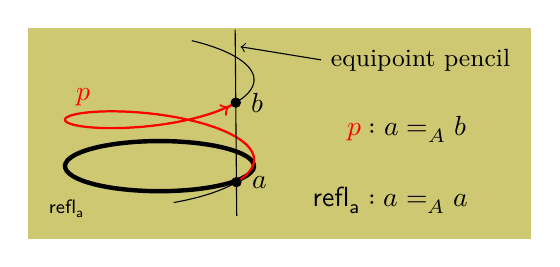
\begin{tikzpicture}[scale=1.0,
    background rectangle/.style={fill=olive!45},
    show background rectangle
  ]
  \begin{axis}[
      view={-20}{-20},
      %% axis line style = ultra thick,
      %% axis lines=middle,
      axis lines=none,
      zmax=80,
      xmax=4,
      ymax=4,
      height=8cm,
      xtick=\empty,
      ytick=\empty,
      ztick=\empty,
      clip=false,
      %% x label style={at={(axis cs:2,0.051)},anchor=north},
      %%   xlabel={$y$},
      %% y label style={at={(axis cs:0.05,2)},anchor=north},
      %%   ylabel={$x$},
      %% z label style={at={(axis cs:0.075,0,80)},anchor=north},
      %%   zlabel={$z$},
    ]
    %% \draw[<-] (-1.2,-5.7) -- node [label={west:foobar}]
    %%      {equality pencil} (0.45,-5.0);

    %% refl a
    \addplot3[samples=30,smooth,variable=t,domain=0:360,ultra thick]
    ({cos(t)},{sin(t)},4.5);
    %% \node [pos=.5,circle,fill]{};
    \node at (-0.5,1.5) [black]{$\mathsf{\scriptstyle refl_a}$};
    \node at (2.6,0) [black]{$\mathsf{refl_a}:a=_A a$};
    \draw [<-] (-0.98,-5.2) -- (0,-5) node [right]
          {\small equipoint pencil};
    %%helix
    \addplot3+[domain=0.5:3*pi,samples=500,samples y=1,
      black,no marks]
    ({sin(deg(x))}, {cos(deg(x))}, {10*x/(pi)});
    %% p:a=b
    \addplot3+[domain=1.3:2.41*pi,samples=500,samples y=1,
      shorten >= 3pt,
      red,->,no marks,thick]
    ({sin(deg(x))},{cos(deg(x))},{10*x/(pi)})%% NB: no semi-colon
    node [name=A,black,circle,scale=0.4,fill,pos=0,
      label={[black,label distance=0pt]east:$a$}]{}
    node [red,pos=0.7,label={north:$p$}]{}
    node [name=B,black,circle,scale=0.4,fill,pos=1,
      label={[black,label distance=0pt]east:$b$}]{};
    %% equality chord
    %%
    \draw[black,shorten >= -1cm, shorten <=-0.5cm] (A)--(B);

\node at (1.8,-2.7) {$\textcolor{red}{p}:a=_Ab$};
\end{axis}
\end{tikzpicture}
\caption{Equality of two distinct values}
\label{fig:aeqb}
%% \end{subcaptiongroup}
%% \begin{subcaptiongroup}{.4\textwidth}
\end{figure}

Figure \ref{fig:aeqb} illustrates proof of equality of two distinct
values. The vertical line (equipoints pencil) represents equality; all
points on the line are equal. The segment joining \(a\) and \(b\)
represents the type \(a=_A b\). The red curve joining \(a\) and \(b\)
(``helical loop'') represents proof that \(a=b\). The black circle
represents \(\textsf{refl}_a:a=a\).

Warning: the vertical equipoints pencil has no counterpart in HoTT; we
just add it for illustrative purposes, to give a graphic
representation of equality types. It makes it look like an equality
proof (helical curve) is just a deformation of an equality type
(straight line), or vice-versa, but that is not the intended meaning.
The equipoints pencil should be thought of as a kind of meta-line.

%% \subcaptionlistentry{Symmetry}
\begin{figure}[h]
\centering
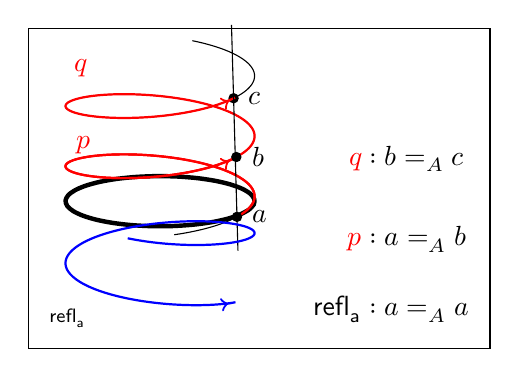
\begin{tikzpicture}[scale=1.0,show background rectangle]
  \begin{axis}[
      view={-20}{-20},
      %% axis line style = ultra thick,
      %% axis lines=middle,
      axis lines=none,
      zmax=80,
      xmax=4,
      ymax=4,
      height=8cm,
      xtick=\empty,
      ytick=\empty,
      ztick=\empty,
      clip=false,
      %% x label style={at={(axis cs:2,0.051)},anchor=north},
      %%   xlabel={$y$},
      %% y label style={at={(axis cs:0.05,2)},anchor=north},
      %%   ylabel={$x$},
      %% z label style={at={(axis cs:0.075,0,80)},anchor=north},
      %%   zlabel={$z$},
    ]
    %% \draw[<-] (-1.2,-5.7) -- node [label={west:foobar}]
    %%      {equality pencil} (0.45,-5.0);

    %% refl a
    \addplot3[samples=30,smooth,variable=t,domain=0:360,ultra thick]
    ({cos(t)},{sin(t)},4.5);
    %% \node [pos=.5,circle,fill]{};
    \node at (-0.5,1.5) [black]{$\mathsf{\scriptstyle refl_a}$};
    \node at (2.6,0) [black]{$\mathsf{refl_a}:a=_A a$};
    %% \draw [<-] (-0.98,-5.2) -- (0,-5) node [right]
    %%       {\small equipoint pencil};
    %%helix
    \addplot3+[domain=0.5:5*pi,samples=500,samples y=1,
      black,no marks]
    ({sin(deg(x))}, {cos(deg(x))}, {10*x/(pi)})
    node [name=C,black,circle,scale=0.4,fill,pos=0.875,
      label={[black,label distance=0pt]east:$c$}]{};

    %% q:b=c
    \addplot3+[domain=1.5:4.41*pi,samples=500,samples y=1,
      shorten >= 3pt,
      red,->,no marks,thick]
    ({sin(deg(x))},{cos(deg(x))},{10*x/(pi)})
    node at (0.7,-5.7) [black] {$\textcolor{red}{q}:b=_Ac$}
    node [red,pos=0.75,label={north:$q$}]{};
    %% p:a=b
    \addplot3+[domain=1.3:2.41*pi,samples=500,samples y=1,
      shorten >= 3pt,
      red,->,no marks,thick]
    ({sin(deg(x))},{cos(deg(x))},{10*x/(pi)})%% NB: no semi-colon
    node [name=A,black,circle,scale=0.4,fill,pos=0,
      label={[black,label distance=0pt]east:$a$}]{}
    node [red,pos=0.7,label={north:$p$}]{}
    node [name=B,black,circle,scale=0.4,fill,pos=1,
      label={[black,label distance=0pt]east:$b$}]{};
    %% equality pencil
    %%
    \draw[black,shorten >= -1cm, shorten <=-0.5cm] (A)--(C);

    \addplot3+[domain=0:2.41*pi,samples=500,samples y=1,
      shorten >= 3pt,
      blue,->,no marks,thick]
    ({sin(deg(x))},{cos(deg(x))},{-10*x/(pi)});

\node at (1.8,-2.7) {$\textcolor{red}{p}:a=_Ab$};

\end{axis}
\end{tikzpicture}
\caption{Transitivity}
\label{fig:transitivity}
%% \end{subcaptiongroup}
%% \captionsetup{subrefformat=parens}
%% \caption{Equality proofs: \subref{fig:peqq} a huge cat,
%% and \subref{fig:aeqb} an elephant}
%% \end{adjustwidth}
\end{figure}

Figure \ref{fig:transitivity} illustrates transitivity.

%% \subcaptionlistentry{Symmetry}
\begin{figure}[h]
\centering
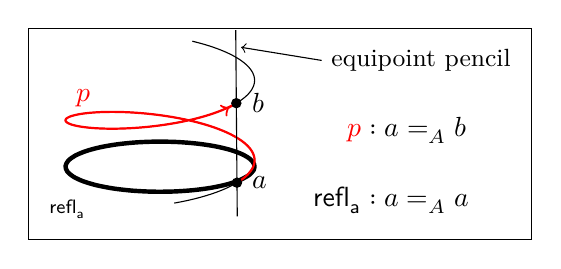
\begin{tikzpicture}[scale=1.0,show background rectangle]
  \begin{axis}[
      view={-20}{-20},
      %% axis line style = ultra thick,
      %% axis lines=middle,
      axis lines=none,
      zmax=80,
      xmax=4,
      ymax=4,
      height=8cm,
      xtick=\empty,
      ytick=\empty,
      ztick=\empty,
      clip=false,
      %% x label style={at={(axis cs:2,0.051)},anchor=north},
      %%   xlabel={$y$},
      %% y label style={at={(axis cs:0.05,2)},anchor=north},
      %%   ylabel={$x$},
      %% z label style={at={(axis cs:0.075,0,80)},anchor=north},
      %%   zlabel={$z$},
    ]
    %% \draw[<-] (-1.2,-5.7) -- node [label={west:foobar}]
    %%      {equality pencil} (0.45,-5.0);

    %% refl a
    \addplot3[samples=30,smooth,variable=t,domain=0:360,ultra thick]
    ({cos(t)},{sin(t)},4.5);
    %% \node [pos=.5,circle,fill]{};
    \node at (-0.5,1.5) [black]{$\mathsf{\scriptstyle refl_a}$};
    \node at (2.6,0) [black]{$\mathsf{refl_a}:a=_A a$};
    \draw [<-] (-0.98,-5.2) -- (0,-5) node [right]
          {\small equipoint pencil};
    %%helix
    \addplot3+[domain=0.5:3*pi,samples=500,samples y=1,
      black,no marks]
    ({sin(deg(x))}, {cos(deg(x))}, {10*x/(pi)});
    %% p:a=b
    \addplot3+[domain=1.3:2.41*pi,samples=500,samples y=1,
      shorten >= 3pt,
      red,->,no marks,thick]
    ({sin(deg(x))},{cos(deg(x))},{10*x/(pi)})%% NB: no semi-colon
    node [name=A,black,circle,scale=0.4,fill,pos=0,
      label={[black,label distance=0pt]east:$a$}]{}
    node [red,pos=0.7,label={north:$p$}]{}
    node [name=B,black,circle,scale=0.4,fill,pos=1,
      label={[black,label distance=0pt]east:$b$}]{};
    %% equality chord
    %%
    \draw[black,shorten >= -1cm, shorten <=-0.5cm] (A)--(B);

\node at (1.8,-2.7) {$\textcolor{red}{p}:a=_Ab$};

\end{axis}
\end{tikzpicture}
\caption{Second-order Equality}
\label{fig:peqq}
%% \end{subcaptiongroup}
%% \captionsetup{subrefformat=parens}
%% \caption{Equality proofs: \subref{fig:peqq} a huge cat,
%% and \subref{fig:aeqb} an elephant}
%% \end{adjustwidth}
\end{figure}

To illustrate second-level equality (figure \ref{fig:peqq}), we would
add a third point \(c\) and a helical loop \(q\) representing proof of
\(b=c\). Then we would shade the region on the surface of the cylinder
between the adjacent helical loops \(p\) and \(q\). This would look
like a ribbon wrapped helically around the cylinder. The surface would
proof of equality of \(p\) and \(q\). This figure would however lack a
graphical representation of the second-level equality type \(p =_{a=_A
  b} q\)

[To really make that work, the ribbon would meta-represent the
  equality type, and the proof would be shown by ``inflating'' the
  ribbon to make a kind of tube.

We can show the three standard properties of the equality relation. We
already show reflexivity. To show symmetry, draw another helical loop
between \(a\) and \(b\), with opposite chirality (polarity). To show
transitivity, draw loops from a to b, and from b to c, and then from a
to c.

\subsection{Codefining Equality}\label{codef_eq}

To codefine equality types, we need three co-constructors:

\begin{itemize}
\item refl: \(x=y \rightarrow x=x\)
\item sym:  \(x=y \rightarrow y=x\)
\item trans: \(x=y, y=z \rightarrow x=z\)
\end{itemize}

Refl is not enough. From any \(p:x=y\) we can derive \(refl:x=x\), but
we have no way to obtain \(q:y=x\) from either, since we have no
constructors for \(x=y\). So we need a co-constructor
\(\mathsf{sym}(p): y=x\).

Ditto for transitivity. We need \(\mathsf{trans}(p,q): x=z\) for
\(p:x=y\) and \(q:y=z\).

These three co-constructors suffice to codefine the entire family of
equality types.

\subsection{Euclidean Equality \\}

Start with the Greeks. First, number. The Greeks had three kinds of
number: quantity, magnitude, and ratio. They did not have an abstract
concept of number that stands apart from these three concepts. A
number was always a number \textit{of} something - length, area, or
volume.

What about angles? We think of them as measureable, but Euclid did
not.

Book I Definition 8 says \enquote{A plane angle is the
  inclination to one another of two lines in a plane which meet one
  another and do not lie in a straight line.}

Book I Definition 10: \enquote{When a straight line set up on a
  straight line makes the adjacent angles equal to one another, each
  of the equal angles is right, and the straight line standing on the
  other is called a perpendicular to that on which it stands.} This
definition presupposes a concept of ``equal angles'', but since
construction of right angles is a basic operation, this amounts to a
definition of both equality and right angle.

Book I Postulate 4: \enquote{That all right angles are equal to one another.}
Obviously a generalization of Book I Definition 10.

But notice that this does not mention \textit{measurement} of angles.
Why not? Presumably because of the way they are constructed.
Measurement of areas and volumes is derived from linear measurement,
starting from a unit length. The unit angle is the right angle; you
don't measure it any more than you measure a unit length. The angle of
a straight line (i.e. 180 degrees) is the sum of two right angles. So
for example a 45 degree angle could not be viewed as a multiple of the
unit angle; it would have to be expressed as a ratio of two angles,
and angular ratios where the unit is the right angle are much more
complicated than linear ratios, where the unit is an arbitrary length.
Note that units cannot be partitioned, so a 45 degree angle cannot be
measured by halving a right angle: ``half'' means ``ratio of two units
to one''.

So in the case of angles, at least, we can have equality without measurement.


Lines, areas, and volumes are incomensurable. A line of length 2 is
not equal to a triangle of area 2. The numbers are different: 2
(units) of length v. 2 (units) of area.

\textquote[\cite{euclid} Book V, ``Theory of Proportions'',
  Proposition 1]{If there be any number of magnitudes whatever which
  are, respectively, equimultiples of any magnitudes equal in
  multitude, then, whatever multiple one of the magnitudes is of one,
  that multiple also will all be of all.}

This tells us we can compare magnitudes of the same kind (lengths,
areas, volumes) by using ratios (``multiples''), and we can compare
ratios across kinds. Proposition 11 makes the latter more explicit:
\enquote{Ratios which are the same with the same ratio are also the
  same with one another.}

Ratios are what allowed the Greeks to compare quantities and
magnitudes. From ``line of length two'' we can derive ``ratio of two
units of length to one unit of length'', and similarly for areas and
volumes. Then we can say that a line and a region have equal measures,
meaning they have equal ratios to their respective unit measures.

Equalities are like ratios. We can ``see'', at least with the mind's
eye, quantities and magnitudes; we cannot see ratios (at least not in
the same direct way). Nor can we see equalities. Moreover, equality is
a concept that applies (equally) to quantities, magnitudes, and
ratios.

\citetitle{euclid} \parencite{euclid}

\begin{enumerate}
\item Things which equal the same thing are also equal to one another.
\item If equals be added to equals, the wholes are equal.
\item If equals be subtracted from equals, the remainders are equal.
\end{enumerate}

Notice that these are not definitions of equality. He never actually
\textit{defines} equality; that is, he does not say what it is for
things to be equals. [TODO: verify] He just tells us what follows from
equality, what inferences we allowed to make \textit{from} equality.

In any case, the point is that for Euclid it makes sense to say of two
\textit{different} things that they are equal. Linear and areal ratios
are ratios \textit{of} different kinds of things, but they may be said
to be equal. So while a line and a square can never be the same thing,
they can be the same ``equimultiple'' of their unit measures.

Modern mathematics began when number was liberated from the prison of
quantity and magnitude. This happened surprisingly late, in the 19th
century, well after mathematicians had begun to use number concepts
that were not easily construed as either quantity or magnitude. For
example, the imaginary number \(i = \sqrt{-1}\) was well-established
before this shift in number concept occurred. Which is to say, that
mathematicians were able to acheive many important results without
having a complete grasp of what they had accomplished. This is
well-known in the case of Euler.

\subsection{Leibniz}

identity of indiscernables v. indiscernability of identicals

\begin{itemize}
\item \citetitle{Abel2020LeibnizEI} \parencite{Abel2020LeibnizEI}
\item \citetitle{10.2307/20016085} \parencite{10.2307/20016085}
\end{itemize}

\subsection{Frege}

\subsection{Russell}

\citetitle{russell_denoting} \cite{russell_denoting}

\textcite[]{If we say ``Scott is the author of Waverley,'' we assert an
  identity of denotation with a difference of meaning. I shall,
  however, not repeat the grounds in favour of this theory, as I have
  urged its claims elsewhere (loc. cit.), and am now concerned to
    dispute those claims.}

\textcite{(1) If a is identical with b, whatever is true of the one is
  true of the other, and either may be substituted for the other in
  any proposition without altering the truth or falsehood of that
  proposition. Now George IV. wished to know whether Scott was the
  author of Waverley; and in fact Scott was the author of Waverley.
  Hence we may substitute Scott for the autlior of " Waverley," and
  thereby prove that George IV. wished to know whether Scott was
  Scott. Yet an interest in the law of identity can hardly be
  attributed to the first gentleman of Europe.}

\subsection{Church}

“things are identical if the name of one can be substituted for
that of the other without loss of truth” (Church 1956, p. 300).

\subsection{Wittgenstein}

Roughly speaking: to say of two things that they are identical is
nonsense, and to say of one thing that it is identical with itself is
to say nothing. (Tractatus?)

\section{Notes}

\subsection{Logical Pluralism}

Is logic one or many? These days there are many logics to choose from.
The question is whether they are all species of a single genus.

To really understand a logic, you must master the use of a calculus. A
calculus for a logic defines the language you use to express reasoning
within the logic. But there are many calculi to choose from, each of
which can be used for different logics. The calculi themselves have
various properties, so they offer different perspectives on reasoning.
So the really \textit{really} understand a logic, you should master
multiple calculi.

We can also ask whether all logical calculi are species of a single
genus. This suggests that the calculi themselves are worthy objects of
study, and the answer is clearly yes. The study of such calculi
usually falls under the rubric ``Proof theory'', but be forewarned
that, as its name suggests, Proof Theory also studies other things,
such the nature of proofs.

We can ask again: are all proofs species of a single genus?

Is there more than one consequence relation? And is consequence the
same as inference?

Finally, we can ask whether all inferences are species of a single
genus. This, like our other questions about logical plurality, is a
philosophical question, whose answer is by no means obvious. For
example, take Classical and Intuitionistic logics. One of the main
differences between them is that the latter includes the Law of
Excluded Middle (LEM)\footnote{Sometimes called the Principle of
Excluded Middle (PEM)}. This law says that every proposition is either
true or false; there is no middle option. So if we do not know whether
a particular proposition \(P\) is true or false, at least we know that
it \textit{must} be one or the other. This means that if we assume it
is false and then prove a contradiction, we not only can but must
\textit{infer} that it is true. Under Intuitionistic logic, things are
different. We can infer that it is not true, but we must not infer
that it is false. Does this difference reflect a \textit{difference in
  kind} of the inferences involved in the two logics?

Variety of form does not entail plurality of content. FOL can be
expressed in many calculi whose forms vary greatly, but they all
express FOL.

See \citetitle{sep-logical-pluralism} \parencite{sep-logical-pluralism}
for more information.


\subsection{Centrality of Inference}

The one thing all logical calculi have in common is a notion
inference. It should be obvious that any calculus we want to use to
express reasoning must have a means of expressing inference, since
inference is the central concept of reasoning. But it's less obvious
that this should be the \textit{only} thing they must have in common.

What about proof? No, that's an add-on; you can have a logical
calculus that does not define what counts as a proof. Most do define
proof formally, but it is not required. Remember that logic is about
consequence, not proof. The concept of proof is parasitic on the
concept of consequence.


\subsection{Residuation}

Bimbó says that operators are residuals of operators, for example
p. 120 says \(\lollipop\) is the residual of \(\circ\) in linear
logic.

But Restall makes it look like residuation is about operands, not
operators.

Must be that \(\vdash\) is the residual of \(→\), or vice versa?


\textquote[\citetitle{sep-logic-substructural} \cite{sep-logic-substructural}]{
Logic is about logical consequence. As a result, the conditional is a central notion in logic because of its intimate connection with logical consequence. This connection is neatly expressed in the residuation condition (also known as the deduction theorem):

\[p,q\vdash r\ \text{if and only if}\ p\vdash q\rightarrow r\]

It says that \(r\) follows from \(p\) together with \(q\) just when \(q→r\)
follows from p alone. The validity of the transition from \(q\) to \(r\)
(given \(p\)) is recorded by the conditional \(q→r\).

This connection between the conditional and consequence is called
residuation by analogy with the case in mathematics. Consider the
connection between addition and substraction. \(a+b=c\) if and only if
\(a=c−b\). The resulting \(a\) (which is \(c−b\)) is the residual,
what is left of \(c\) when \(b\) is taken away. Another name for this
connection is the deduction theorem.}

The term makes perfect sense for arithmetic. It is a standard term in
statistics, where the residual is the difference between an predicted
and observed values. But its harder to see how to give it an intuitive
reading in logic. It seems to be motivated by formal analogy:

\begin{align}
  a+b &= c & \text{arithmetic sum equals c} \\
  a &= c - b & \text{arithmetic residual equals difference} \\
  b &= c - a \\
  p,q &\vdash c & \text{sum entails c} \\
  p &\vdash q→r & \text{residual p entails implication} \\
  q &\vdash p→r
\end{align}

The formal analogy is clear, but it's hard to see how arithmetic
difference and implication are related. But I think the formal analogy
does reflect substantial analogy.

The arithmetic residual is what you get when you ``undo'' a sum. Just
focus on the LHS: the residual is what you get when you remove a
summand. But what makes it a ``residual'', instead of just a summand?
The relation of addition and subtraction on the one hand, and equality
on the other. Residuation expresses that link.

Or: residuation preserves equality. If you remove one of the summands,
what do you need to do to restore equality? Make that move and the remaining summand is a residual.

So in logic: residuation preserves entailment. If you remove one of
the conjuncts from the antecedent, what do you need to do to preserve
the entailment?  You convert the conclusion to an implication. So conjunction is the residual of implication.

Better: residuation as an algebraic (-like) operation whose purpose is
to restore inferential equilibrium. If you break the whole, by
removing a part on the left, then to mend (al-jabr) and restore the
balance (al-muqabala) you must treat the RHS. In the case of ``and''
on the LHS, the remedy is to introduce a new operator, \(→\), on the
RHS.

Restall seems to get this wrong, calling residuation a relation
between the conditional and consequence. I think it is a relation
between two operators mediated by consequence. After all the
conditional is not the only operator that can be entailed; in fact
they are all essentially related to entailent. The general form: if
you remove an operand on the LHS, what do you need to do on the RHS in
order to preserve the entailment? The answer will involve another
operation.

For logic, the residual \(p\) is what you get when you remove the
summand (or ``factor''?) \(q\) from the sum \(\ulcorner
p,q\urcorner\). What makes it a residual instead of a mere premise?
The relation between summing (\(\ulcorner ,\urcorner\)) and
implication.

In a real sense is it is a lack. Remove one of the conditions of
production and the output lacks something.

Treat \(p,q\vdash r\) as a binary function. If you want to convert it
to a unary function, you remove one of the parameters, and you output
another unary function that takes the removed parameter as its arg.

In other words, this kind of residuation is just currying. Which makes
the deduction theorem a kind of currying. The residual is the
second-level (``wrapped'') unary function.

How nice, this gives us a piece of terminology we can use to talk
about currying. For each parameter of any binary function, we have a
residual, which is the unary function that takes the other parameter
as an argument. E.g. if we have \(f(a,b)→c\), then the residual of
\(a\) is the unary function that takes \(b\) as an argument (and may
also use a, but not as an arg) and returns \(c\).

For arithmetic, residuals are numbers. For logic, they are operators.
Implication is the residual of conjunction, because it is what you
need to restore entailment after you remove conjunction. Its ``what's
left over'' after removal of conjunction.

This is incredibly obvious once you see it. Why did it take me so long
to see it?

Are residuals always implication operators? Seems they must be; to
restore entailment, you must add implication.

\begin{itemize}
\item \(a + b = c\) the arithmetic sum of a and b equals c.
\item \(a = c - b\) the residual a is what's left when you subtract b from c
\item \(p,q\vdash r\) the logical sum of p and q entails r
\item \(p\vdash q→r\): p is what is left when you ...?
\end{itemize}

Here ``logical sum'' does not mean ``logical conjunction''
(\(\land\)). It is meant to convey the ``structural'' concept of ``p and
q together'' \textit{outside} of the logic.

The algebraic operation that yields the residual is the same on both
sides of the equation symbol. But the logical operation is not; it's
not even symmetrical.  To get the residual, we need to:

\begin{itemize}
\item remove \(q\) from the sum on the LHS
\item combine it (``add'' it?) on the RHS in a particular way
\end{itemize}

\subsection{Arbitary Choice Operator}

These calculi depend heavily on assumptions. The premises of inference rules are assumptions. For type systems, they look like \(a:A\), i.e. assume a is of type A.  More explicitly, assume A is non-empty and a is an \textit{arbitrary} token of type A.

Currently square brackets are used to make assumptions explicit, but
they are also used for other purposes.

We can make this more explicity by defining a choice operator. For
example, we can borrow Hilbert's epsilon. Then \(\epsilon \phi\) would
mean ``choose arbitrary proposition \(\phi\)'', and \(\epsilon a:A\)
would mean ``choose arbitrary a of type A''. Same as the assumption
above, but explicit.

Examples:

\begin{center}
\AxiomC{$\Gamma$}
\AxiomC{$[\phi]$}
\noLine
\UnaryInfC{$\vdots$}
\noLine
\UnaryInfC{$\psi$}
\BinaryInfC{$\phi\rightarrow\psi$}
\DisplayProof
\hskip1em
\rightarrow
\AxiomC{$\Gamma$}
\AxiomC{$\epsilon\phi$}
\noLine
\UnaryInfC{$\vdots$}
\noLine
\UnaryInfC{$\psi$}
\BinaryInfC{$\phi\rightarrow\psi$}
\DisplayProof
\end{center}

With types:

\begin{center}
\AxiomC{$\Gamma$}
\AxiomC{$[\phi:A]$}
\noLine
\UnaryInfC{$\vdots$}
\noLine
\UnaryInfC{$\psi:B$}
\BinaryInfC{$\phi\rightarrow\psi:$}
\DisplayProof
\hskip1em
\rightarrow
\AxiomC{$\Gamma$}
\AxiomC{$\epsilon\phi$}
\noLine
\UnaryInfC{$\vdots$}
\noLine
\UnaryInfC{$\psi$}
\BinaryInfC{$\phi\rightarrow\psi$}
\DisplayProof
\end{center}

\subsection{Disjunction}

We actually need a choice operator to make sense of disjunction, or
more precisely, to make our calculus work for disjunction.

To see why, start with conjunction: \(A, B\vdash A\lkand B\). The
usual way to gloss this is something like ``If A is true and B is
true, then A\(\lkand\) B is true''. But we need to be more explicit.
Implicit in the standard gloss is that A and B are
propositions.\footnote{TODO: note on Martin-Löf}. Also implicit is
universal quantification; what we really mean is ``For all
propositions A and B, if A is true and B is true, then A\(\lkand\) B
is true''.

Note that in \(A, B\vdash A\lkand B\) the only symbol in the
conclusion that is not in the premises is \(\lkand\).

To make the interpretation of such formulae fully explicit, we have
two options. We can use the universal quantifier, and write something
like \(\forall A, B: A, B\seqso A\lkand B\). Or we can use our choice
operator, and write \(\choice A, \choice B\seqso A\lkand
B\).\footnote{Read ``if arbitrary A is true and arbitrary B is true
then A\lkand B is true''.} But this leaves the domain of
quantification implicit; the be really explicit, we would have to find
a way to indicate that A and B range over propositions (for
\(\forall\)), and that \(\choice A\) means ``for arbitrary proposition
A''.

Now look at the standard introduction rules for disjunction. We have
two, one for the left disjunct and one for the right: \(A\seqso A\lkor
B\) and \(B\seqso A\lkor B\). The problem is immediately evident:
\(B\) appears in the conclusion but not in the premises. The rules
introduce more than just \(\lkor\); they also introduce \(B\). But
\(B\) is a non-logical symbol, so this makes no sense.

The implicit logic is simple enough. We take \(A\seqso A\lkor B\) to
mean ``If A is true, then A\lkor B is true whether B is true or not'';
more precisely, ``For all propopsitions A, if A is true, then for all
propositions B, \(A\lkor B\) is true''. In other words, to make sense
of the introduction rules for disjunction, we're forced to commit to
\textit{two} implicit universal quantifications. Symbolically, using
\(\ulcorner :\mathbb{P}\urcorner\) to mean ``ranging over
propositions'':

\[\forall A:\mathbb{P}, A\seqso\forall B:\mathbb{P}, A\lkor B\]

But this is cumbersome.  Using \(\choice\) we get a more concise expression

\[\choice A\seqso A\lkor \choice B\]

But now we're back where we started: the conclusion contains symbols
that are not in the premises. What we need is a way to mention \(B\)
in the premises. If we try \(\choice B\), then we get the same
premises as the introduction rule for \(\lkand\). That's because we
read the meta-symbol \(\ulcorner ,\urcorner\) as ``and'', so when use
as premise(s) \(\ulcorner\choice A,\choice B\urcorner\) must be
glossed ``if arbitrary A is true and arbitrary B is true'', and this
gives us the wrong scope of quantification for disjunction. We need to
quantify B \textit{after} A, or choose arbitrary \(B\) \textit{after}
we've chosen arbitrary \(A\). But that means that \(B\)
\textit{cannot} be involved in the premise, which in turn suggests
that it must be the introduction rule itself that injects, not just
symbol \(B\), but also its quantification.

In other words, ``natural'' \(\lkor\), the kind defined by
introduction and elimination rules, presupposes a subordinate
quantification. It follows that the introduction rules do more than
just introduce the logical constant. But that's ok. Nothing says that
such rules must introduce the constant \textit{and nothing else}. The
only constraint is that the additional ``stuff'' introduced must not
have any ``side effects'', that is must not turn any other good
inferences into bad ones or vice-versa. Which is to say, each
introduction rule must be a \textit{conservative extension} of the
language.

Who cares? Why bother, except to make the logic fully explicit? Well,
a finer degree of explicitation is not nothing. In this case, it will
help us better understand typed calculi.

\subsection{Vernacular}

The vernacular is the language of prelogic.

The vernacular is not meta-logic. It uses logic, but is not
\textit{about} logic.

\subsection{Proof Theory}

\textquote[\citetitle{DBLP:journals/sLogica/Prawitz19} \cite{DBLP:journals/sLogica/Prawitz19}]{I see the question
  what it is that makes an inference valid and thereby gives a proof
  its epistemic power as the most fundamental problem of general proof
  theory.
  \vskip-2em
  \[\vdots\]
  \vskip-1em
  ``In my plea for general proof theory, I suggested a number of obvious topics: the question of defining the concept of proof, investigations of the structure of proofs, the representation of proofs by formal derivations, and the finding of identity criteria of proofs that answered the question when two derivations represent the same proof.
  \vskip-2em
  \[\vdots\]
  \vskip-1em
  ``But I still think that the problem of defining the concept of proof or the validity of inference is the most fundamental problem of general proof theory...
}

Remember that the concept of proof presupposes a concept of
consequence (or inference), so a theory of proof lives or dies by its
notion of consequence.

Proof is usually defined as (roughly) a tree or chain or anyway
structure of ``connected'' inferences, expressed as derivation
structure in the calculus.

\subsection{Proof Identity}

We can have different proofs for the same proposition. How can we tell
if they are equal? This is an unsolved problem. But it accounts for
the complexity of equality in HoTT.

Compare: deciding when two functions are equal, that is, when two
implementations of the same function are equal. We know the criteria
for deciding: same outputs for same inputs. But its possible that two
different algorithms could accomplish that. Would they count as the
identical? Extensionally, yes; intensionally, no. Do they need to be
the same program?

\subsection{Proof-irrelevance}
Propositions are forgetful. They do not remember how they came to be.
E.g. \(A\land B\) does not know that it was formed using the intro
rule. In fact there is no reason to assume that it was. This is easier
to see in a type system, where we would have \(p:A\times B\), meaning
that \(p\) is a token (term, instance, etc.) of type \(A\times B\), or
equivalently \(p\) is a proof of the type. This tells us nothing about
how \(p\) came to be.

\subsection{Closed-World Assumption}



\subsection{Codefinition}

Introduction (right) rules define; elimination (left) rules co-define.
Elimination rules make an assumption, that the proposition they are
using is ``defined''. But that is just an assumption. The elimination
rule itself says what can be done with the propositon, but this cannot
count as a definition \textit{of} the proposition. Definitions, under
this perspective, tell us how things are put together. They do not
tell us how to \textit{use} what we have put together; in particular
they to not tell us how to disassemble composites.

Codefinitions do that. They tell us what we can do with the composite,
\textit{on the assumption} that it is already ``defined'' in some
indeterminate way. But they do \textit{not} assume that is was
constructed by an introduction rule.

Take \(\land\) for example. Here is the way the rules are often
presented, with the context and \(\vdash\) omitted for simplicity's
sake:

%% Logical And
\begin{center}
\AxiomC{$A$}
\AxiomC{$B$}
\BinaryInfC{$A\land B$}
\DisplayProof
\hskip 1.4em
\AxiomC{$A\land B$}
\UnaryInfC{$A$}
\DisplayProof
\hskip 1.4em
\AxiomC{$A\land B$}
\UnaryInfC{$B$}
\DisplayProof
\end{center}

The rule on the left defines \(A\land B\): you build a conjunct
\(A\land B\) from an A and a a B. The two on the right jointly
co-define it: given (that is, \textit{assuming}) \(A\land B\), you
can extract A or B or both.

This example is a bit misleading, though, since the syntax \(A\land
B\) suggests that the elimination rules operate by extracting A or B
syntactically. That is not the case. We can make this more evident by
rewriting the rules as follows to make the assumptions explicit:

\begin{center}
  \AxiomC{$P$}
  \LeftLabel{$\scriptstyle\text{[P a \(\land\) conjunct]}$}
  \UnaryInfC{$first(P)$}
  \DisplayProof
  \hskip 1.4em
  \AxiomC{$P$}
  \LeftLabel{$\scriptstyle\text{[P a conjunction]}$}
  \UnaryInfC{$second(P)$}
  \DisplayProof
\end{center}

In type theories, conjunction corresponds to product types:

\begin{center}
  \AxiomC{$p:A\times B$}
  \UnaryInfC{$first(p):A$}
  \DisplayProof
  \hskip 1.4em
  \AxiomC{$p:A\times B$}
  \UnaryInfC{$second(p):B$}
  \DisplayProof
\end{center}

In other words, the elimination rules tell us that we can extract a ``first'' element and a ``second'' element from any conjunct.

To make this work we also need to \textit{harmonize} the definition
and co-definition. In this case that means ensuring that we can
control which element we extract. The definitional introduction rule
says we can combine A and B; the codefinitional rules must allow us to
reliably retrieve either one. In other words, we need to ensure that
if we construct \(A\land B\), then \(first\) will extract A.

In the case of our first example, this is already evident from the
syntax of the rules. But if we want to use the second style, we cannot
depend on the meanings of \(first\) and \(second\) to guarantee this;
after all, we could have used some other terms, such as \textit{left}
and \textit{right}, \textit{red} and \textit{blue}, or even
\textit{foo} and \textit{bar}. Whatever terms we use, we need to
establish a corresponds between the eliminator terms and the
constructor. The only way to do this is by setting down a meta-axiom
that says that the first argument to the constructor corresponds to
one extractor, and the second to the other. Something like this
\(red(A\land B)\eqdef A\), \(blue(A\land B)\eqdef B\)

Note: the extractors (\textit{first}, \textit{second}, or whatever)
use function application syntax, but they are not functions. They are
codefiners \textit{by} definition, but do not themselves \textit{have}
definitions.

Usually this harmonization is taken for granted, because its obvious
and tedious to write out.


%%%%%%%%%%%%%%%%%%%%%%%%%%%%%%%%%%%%%%%%%%%%%%%%%%%%%%%%%%%%%%%%
%%%%%%%%%%%%%%%%%%%%%%%%%%%%%%%%%%%%%%%%%%%%%%%%%%%%%%%%%%%%%%%%
\section{Appendix: The Calculi}

%%%%%%%%%%%%%%%%
\subsection{Natural Deduction}

%% Logical And
\begin{center}
\AxiomC{$A\kern-1.2em$}
\AxiomC{$B$}
\RightLabel{$\scriptstyle{[\land \textrm{-intro}]}$}
\BinaryInfC{$A\land B$}
\DisplayProof
\hskip 1.4em
\AxiomC{$A\land B$}
\RightLabel{$\scriptstyle{[\land\ \text{-exit}_{\text{L}}]}$}
\UnaryInfC{$A$}
\DisplayProof
\hskip 1.4em
\AxiomC{$A\land B$}
\RightLabel{$\scriptstyle{[\land\ \text{-exit}_{\text{R}}]}$}
\UnaryInfC{$B$}
\DisplayProof
\end{center}

%%%%%%%%%%%%%%%%
\subsection{LK}

First some helpful vocabulary:

\begin{description}
\item[Sequent]
  \item[Antecedent] The part of a sequent preceding \(\vdash\).
  \item[Consequent] The part of a sequent following \(\vdash\).
  \item[Principle formula] The (sub-)formula containing the logical
    constant being defined. For example, in rule \(\land\vdash\), the
    principle formula is \mbox{\(A\land B,\Gamma\vdash \Delta\)}.
  \item[Structure] A sequence of formulae. Uppercase Greek letters
    \(\Gamma, \Delta, \Theta, \Sigma\), etc. are used as
    meta-variables to represent sequences of formulae, which may be
    combined with formula meta-variables (\(A, B, C, etc.\)); for
    example, \(\ulcorner A,\Gamma\urcorner\) and \(\ulcorner \Gamma,
    A\urcorner\) are structures.
    \item[Structure connectives] There is only one structure
      connective: comma. Represents conjunction (\(\land\)) in
      antecedents and disjunction (\(\lor\)) in consequents.
    \item[Sequent connective] There are two sequent connectivess,
      \(\seqand\), meaning ``and also'' and \(\seqor\), meaning
      ``either\ldots or''. A rule that uses \(\seqor\) represents the
      merger of two separate rules; most presentations of the calculus
      list them separately and do not use an explicit sequent
      connective. In most presentations of sequent calculi, sequent
      connectives are not made explicit, but making them explicit
      brings out features, especially symmetries, that otherwise may
      not be so clear.
    \item[Logical connectives] The usual logical constants: \(\land,
      \lor\), etc.
\end{description}

By convention, rules are categorized as left or right, depending on 1)
the location of the principle formula on the bottom; and 2) the
location of the propositional variables in the sequents. For example,
rule \(\land\vdash\) is the left rule for \(\land\).

Left rules correspond to elimination rules, right rules, to
introduction rules. We want the introduction rules on the left, since
by convention they are usually presented before elimination rules.
This means that right rules are in the left column here.

Left rules show that when the principle formula is an antecedent of a
bottom sequent (i.e. the conclusion of an inference), inference to the
consequent may be acheived by decomposing it and using one of the
sequents in the premise to make the inference. I.e. it represents a
kind of backward reasoning.

\subsubsection{Axioms}

%% Id, Cut
\begin{center}
\AxiomC{}
\RightLabel{$\text{Id}$}
\UnaryInfC{$A\land A$}
\DisplayProof
\hskip 1.4em
\AxiomC{$\Gamma\vdash \Delta_1,C,\Delta_2\kern-1.2em$}
\AxiomC{$\seqand\kern-1.2em$}
\AxiomC{$\Theta_1,C,\Theta_2\vdash\Lambda$}
\RightLabel{$\text{cut}$}
\TrinaryInfC{$\Theta_1,\Gamma,\Theta_2\vdash \Delta_1,\Lambda,\Delta_2$}
\DisplayProof
\end{center}

\subsubsection{Logical Rules}

Also called (by Bimbó) operational rules.

%% Logical And
\begin{center}
\AxiomC{$\Gamma\vdash \Delta, A\kern-1.2em$}
\AxiomC{$\seqand\kern-1.2em$}
\AxiomC{$\Gamma\vdash \Delta, B$}
\RightLabel{$\vdash\land$}
\TrinaryInfC{$\Gamma\vdash \Delta, A\land B$}
\DisplayProof
\hskip 1.4em
\AxiomC{$A,\Gamma\vdash \Delta\kern-1.2em$}
\AxiomC{$\seqor\kern-1.2em$}
\AxiomC{$B,\Gamma\vdash \Delta$}
\RightLabel{$\land\vdash$}
\TrinaryInfC{$A\land B,\Gamma\vdash \Delta$}
\DisplayProof
\end{center}

%% Logical Or
\begin{center}
\AxiomC{$\Gamma\vdash \Delta, A\kern-1.2em$}
\AxiomC{$\seqor\kern-1.2em$}
\AxiomC{$\Gamma\vdash \Delta, B$}
\RightLabel{$\vdash\lor$}
\TrinaryInfC{$\Gamma\vdash\Delta, A\lor B$}
\DisplayProof
\hskip 1.4em
\AxiomC{$A,\Gamma\vdash \Delta\kern-1.2em$}
\AxiomC{$\seqand\kern-1.2em$}
\AxiomC{$B,\Gamma\vdash \Delta$}
\RightLabel{$\lor\vdash$}
\TrinaryInfC{$A\lor B,\Gamma\vdash \Delta$}
\DisplayProof
\end{center}

%% Implication
\begin{center}
\AxiomC{$A,\Gamma\vdash \Delta,B\kern-1.2em$}
\RightLabel{$\vdash\supset$}
\UnaryInfC{$\Gamma\vdash \Delta,A\supset B$}
\DisplayProof
\hskip 1.4em
\AxiomC{$\Gamma\vdash \Delta, A\kern-1.2em$}
\AxiomC{$\seqand\kern-1.2em$}
\AxiomC{$B,\Theta\vdash \Lambda$}
\RightLabel{$\supset\vdash$}
\TrinaryInfC{$A\supset B,\Gamma,\Theta\vdash\Delta,\Lambda$}
\DisplayProof
\end{center}

%% Not
\begin{center}
\AxiomC{$A,\Gamma\vdash \Delta\kern-1.2em$}
\RightLabel{$\vdash\neg$}
\UnaryInfC{$\Gamma\vdash \Delta,\neg A$}
\DisplayProof
\hskip 1.4em
\AxiomC{$\Gamma\vdash \Delta, A\kern-1.2em$}
\RightLabel{$\neg\vdash$}
\UnaryInfC{$\neg A,\Gamma\vdash\Delta$}
\DisplayProof
\end{center}

%% Universal quantification
\begin{center}
\AxiomC{$A,\Gamma\vdash \Delta\kern-1.2em$}
\RightLabel{$\vdash\forall$}
\UnaryInfC{$\Gamma\vdash \Delta,\neg A$}
\DisplayProof
\hskip 1.4em
\AxiomC{$\Gamma\vdash \Delta, A\kern-1.2em$}
\RightLabel{$\forall\vdash$}
\UnaryInfC{$\neg A,\Gamma\vdash\Delta$}
\DisplayProof
\end{center}

%% Existential quantification
\begin{center}
\AxiomC{$A,\Gamma\vdash \Delta\kern-1.2em$}
\RightLabel{$\vdash\exists$}
\UnaryInfC{$\Gamma\vdash \Delta,\neg A$}
\DisplayProof
\hskip 1.4em
\AxiomC{$\Gamma\vdash \Delta, A\kern-1.2em$}
\RightLabel{$\exists\vdash$}
\UnaryInfC{$\neg A,\Gamma\vdash\Delta$}
\DisplayProof
\end{center}


\subsubsection{Structural Rules}

%% thinning
\begin{center}
\AxiomC{$\Gamma\vdash \Delta\kern-1.2em$}
\RightLabel{$\vdash\text{K}$}
\UnaryInfC{$\Gamma\vdash \Delta, A$}
\DisplayProof
\hskip 1.4em
\AxiomC{$\Gamma\vdash \Delta\kern-1.2em$}
\RightLabel{$\text{K}\vdash$}
\UnaryInfC{$A,\Gamma\vdash\Delta$}
\DisplayProof
\end{center}

%% contraction
\begin{center}
\AxiomC{$\Gamma\vdash \Delta, A, A$}
\RightLabel{$\vdash\text{W}$}
\UnaryInfC{$\Gamma\vdash\Delta, A$}
\DisplayProof
\hskip 1.4em
\AxiomC{$A,A,\Gamma\vdash \Delta$}
\RightLabel{$\text{W}\vdash$}
\UnaryInfC{$A,\Gamma\vdash \Delta$}
\DisplayProof
\end{center}

%% Exchange
\begin{center}
\AxiomC{$\Theta\vdash\Gamma,A,B,\Delta$}
\RightLabel{$\vdash\text{C}$}
\UnaryInfC{$\Theta\vdash\Gamma,B,A,\Delta$}
\DisplayProof
\hskip 1.4em
\AxiomC{$\Gamma,A,B,\Delta\vdash\Theta$}
\RightLabel{$\text{C}\vdash$}
\UnaryInfC{$\Gamma,B,A,\Delta\vdash\Theta$}
\DisplayProof
\end{center}

\subsection{Notes}

Source: \textquote[\parencite{bimbo2014proof}]{Proof Theory: Sequent Calculi and Related Formalisms}

\subsection{LL}

Source: \parencite{Girard95linearlogic}, p. 10

\subsubsection{Notation}

We use custom symbols in order to bring the meanings more clearly to
the surface.

\begin{itemize}
\item Additive conjunction: \(A \addand B\). You have both A
  \textit{and} B, but you can only use one: A \textit{or} B.
\item Additive disjunction: \(A \addor B\)
\item Multiplicative conjunction: \(A\fusion B\). You have both, and
  you can only use both together to produce a single output. Alternatively, you can only use it as input to rules that need both.
\item Multiplicative disjunction: \(A\fission B\). You have both, and
  you can use A or B or both to produce either of two possible outputs.
\end{itemize}



\subsubsection{Axioms}

%% Id, Cut
\begin{center}
\AxiomC{}
\RightLabel{$\text{Id}$}
\UnaryInfC{$A\land A$}
\DisplayProof
\hskip 1.4em
\AxiomC{$\Gamma\vdash \Delta_1,C,\Delta_2\kern-1.2em$}
\AxiomC{$\seqand\kern-1.2em$}
\AxiomC{$\Theta_1,C,\Theta_2\vdash\Lambda$}
\RightLabel{$\text{cut}$}
\TrinaryInfC{$\Theta_1,\Gamma,\Theta_2\vdash \Delta_1,\Lambda,\Delta_2$}
\DisplayProof
\end{center}

\subsubsection{Logical Rules}

Also called (by Bimbó) operational rules.

%% Logical And
\begin{center}
\AxiomC{$\Gamma\vdash \Delta, A\kern-1.2em$}
\AxiomC{$\seqand\kern-1.2em$}
\AxiomC{$\Gamma\vdash \Delta, B$}
\RightLabel{$\vdash\land$}
\TrinaryInfC{$\Gamma\vdash \Delta, A\land B$}
\DisplayProof
\hskip 1.4em
\AxiomC{$A,\Gamma\vdash \Delta\kern-1.2em$}
\AxiomC{$\seqor\kern-1.2em$}
\AxiomC{$B,\Gamma\vdash \Delta$}
\RightLabel{$\land\vdash$}
\TrinaryInfC{$A\land B,\Gamma\vdash \Delta$}
\DisplayProof
\end{center}

%% Logical Or
\begin{center}
\AxiomC{$\Gamma\vdash \Delta, A\kern-1.2em$}
\AxiomC{$\seqor\kern-1.2em$}
\AxiomC{$\Gamma\vdash \Delta, B$}
\RightLabel{$\vdash\lor$}
\TrinaryInfC{$\Gamma\vdash\Delta, A\lor B$}
\DisplayProof
\hskip 1.4em
\AxiomC{$A,\Gamma\vdash \Delta\kern-1.2em$}
\AxiomC{$\seqand\kern-1.2em$}
\AxiomC{$B,\Gamma\vdash \Delta$}
\RightLabel{$\lor\vdash$}
\TrinaryInfC{$A\lor B,\Gamma\vdash \Delta$}
\DisplayProof
\end{center}

%% Implication
\begin{center}
\AxiomC{$A,\Gamma\vdash \Delta,B\kern-1.2em$}
\RightLabel{$\vdash\supset$}
\UnaryInfC{$\Gamma\vdash \Delta,A\supset B$}
\DisplayProof
\hskip 1.4em
\AxiomC{$\Gamma\vdash \Delta, A\kern-1.2em$}
\AxiomC{$\seqand\kern-1.2em$}
\AxiomC{$B,\Theta\vdash \Lambda$}
\RightLabel{$\supset\vdash$}
\TrinaryInfC{$A\supset B,\Gamma,\Theta\vdash\Delta,\Lambda$}
\DisplayProof
\end{center}

%% Not
\begin{center}
\AxiomC{$A,\Gamma\vdash \Delta\kern-1.2em$}
\RightLabel{$\vdash\neg$}
\UnaryInfC{$\Gamma\vdash \Delta,\neg A$}
\DisplayProof
\hskip 1.4em
\AxiomC{$\Gamma\vdash \Delta, A\kern-1.2em$}
\RightLabel{$\neg\vdash$}
\UnaryInfC{$\neg A,\Gamma\vdash\Delta$}
\DisplayProof
\end{center}

%% Universal quantification
\begin{center}
\AxiomC{$A,\Gamma\vdash \Delta\kern-1.2em$}
\RightLabel{$\vdash\forall$}
\UnaryInfC{$\Gamma\vdash \Delta,\neg A$}
\DisplayProof
\hskip 1.4em
\AxiomC{$\Gamma\vdash \Delta, A\kern-1.2em$}
\RightLabel{$\forall\vdash$}
\UnaryInfC{$\neg A,\Gamma\vdash\Delta$}
\DisplayProof
\end{center}

%% Existential quantification
\begin{center}
\AxiomC{$A,\Gamma\vdash \Delta\kern-1.2em$}
\RightLabel{$\vdash\exists$}
\UnaryInfC{$\Gamma\vdash \Delta,\neg A$}
\DisplayProof
\hskip 1.4em
\AxiomC{$\Gamma\vdash \Delta, A\kern-1.2em$}
\RightLabel{$\exists\vdash$}
\UnaryInfC{$\neg A,\Gamma\vdash\Delta$}
\DisplayProof
\end{center}


\subsubsection{Structural Rules}

%% thinning
\begin{center}
\AxiomC{$\Gamma\vdash \Delta\kern-1.2em$}
\RightLabel{$\vdash\text{K}$}
\UnaryInfC{$\Gamma\vdash \Delta, A$}
\DisplayProof
\hskip 1.4em
\AxiomC{$\Gamma\vdash \Delta\kern-1.2em$}
\RightLabel{$\text{K}\vdash$}
\UnaryInfC{$A,\Gamma\vdash\Delta$}
\DisplayProof
\end{center}

%% contraction
\begin{center}
\AxiomC{$\Gamma\vdash \Delta, A, A$}
\RightLabel{$\vdash\text{W}$}
\UnaryInfC{$\Gamma\vdash\Delta, A$}
\DisplayProof
\hskip 1.4em
\AxiomC{$A,A,\Gamma\vdash \Delta$}
\RightLabel{$\text{W}\vdash$}
\UnaryInfC{$A,\Gamma\vdash \Delta$}
\DisplayProof
\end{center}

%% Exchange
\begin{center}
\AxiomC{$\Theta\vdash\Gamma,A,B,\Delta$}
\RightLabel{$\vdash\text{C}$}
\UnaryInfC{$\Theta\vdash\Gamma,B,A,\Delta$}
\DisplayProof
\hskip 1.4em
\AxiomC{$\Gamma,A,B,\Delta\vdash\Theta$}
\RightLabel{$\text{C}\vdash$}
\UnaryInfC{$\Gamma,B,A,\Delta\vdash\Theta$}
\DisplayProof
\end{center}

%%%%%%%%%%%%%%%%%%%%%%%%%%%%%%%%%%%%%%%%%%%%%%%%%%%%%%%%%%%%%%%%
\addcontentsline{toc}{section}{References}
\nocite{*}
\printbibliography

\end{document}
